%%%%%%%%%%%%%%%%%%%%%%%%%%%%%%%%%%%%%%%%%%%%
%                                          %
%  Plantilla para Proyecto Fin de Carrera  %
%                                          %
%%%%%%%%%%%%%%%%%%%%%%%%%%%%%%%%%%%%%%%%%%%%

%
% CONFIG: Definici�n del estilo del documento
%

\documentclass[a4paper,12pt]{Config/itsas_pfc}

%
% CONFIG: Fichero con configuraci�n opcional
%

%
% Paquetes que pueden serte de utilidad (rec = recomendado, opc = opcional)
%
\usepackage{fancyhdr}          % (rec)  permite cambiar varios par�metros de las cabeceras y pi�s de p�gina
\usepackage{courier}           % (opc)  usa esta fuente por defecto
\usepackage{setspace}          % (opc)  permite cambiar el espaciado entre l�neas
\usepackage{longtable}         % (opc)  permite que las tablas ocupen varias p�ginas
\usepackage{lscape}            % (opc)  permite el uso del comando \landscape, para poner algo apaisado
\usepackage{color}             % (opc)  varios comandos relativos al color (como \color)
\usepackage{rotating}          % (opc)  permite rotar PSs y EPSs
\usepackage{textcomp}          % (opc)  permite incluir el s�mbolo del euro, con \texteuro
\usepackage{minitoc}           % (opc)  permite incluir ToCs (�ndice de materias) para cada cap�tulo
\usepackage{epsf}              % (opc)  permite ciertas manipulaciones a EPSs
\usepackage[absolute]{textpos} % (rec)  permite posicionado arbitrario de texto (necesario para la portada)
\usepackage{srcltx}            % (opc)  permite pasar del .dvi al .tex
\usepackage[Config/spanish5, es-tabla]{babel}   % (rec)  da soporte para castellano a LaTeX
\usepackage[latin1]{inputenc}  % (opc)  permite introducir caracteres como �, etc, en el input
\usepackage{caption}
\usepackage{subcaption}
\usepackage{float}
\usepackage{amssymb}
\usepackage{booktabs}% http://ctan.org/pkg/booktabs
\usepackage{listings}
\usepackage{color}
\usepackage{slashbox}
\usepackage{graphicx}
\usepackage{multirow}
\usepackage{array,booktabs}
\usepackage[pdfpagelayout=TwoPageRight, bookmarksnumbered=true]{hyperref}
\usepackage{bookmark}
\usepackage[nottoc]{tocbibind}
\usepackage[titletoc]{appendix}
\usepackage{pdfpages}


\makeatletter
\def\toclevel@chapter{-1}
\makeatother

\newcolumntype{M}[1]{>{\centering\arraybackslash}m{#1}}

\definecolor{dkgreen}{rgb}{0,0.6,0}
\definecolor{gray}{rgb}{0.5,0.5,0.5}
\definecolor{mauve}{rgb}{0.58,0,0.82}

\lstset{frame=tb,
	language=C++,
	aboveskip=3mm,
	belowskip=3mm,
	showstringspaces=false,
	columns=flexible,
	basicstyle={\small\ttfamily},
	numbers=none,
	numberstyle=\tiny\color{gray},
	keywordstyle=\color{blue},
	commentstyle=\color{dkgreen},
	stringstyle=\color{mauve},
	breaklines=true,
	breakatwhitespace=true,
	tabsize=3
}

\newcommand{\tabitem}{~~\llap{\textbullet}~~}
%
% Settings para los m�rgenes. Descomenta y modifica si sabes lo que haces. N�tese
% que a los valores dados se les a�ade una pulgada extra. Los valores dados son los
% predeterminados para papel A4 y el estilo itsas_pfc.cls.
%
%\setlength{\oddsidemargin}{10pt}     % m�rgen izquierdo para p�ginas impares (izquierda)
%\setlength{\evensidemargin}{52pt}    % m�rgen izquierdo para p�ginas pares (derecha)
%\setlength{\textwidth}{390pt}        % anchura del cuerpo de texto

%
% Recomendado para mejorar la colocaci�n autom�tica de las figuras.
% (tomado de http://dcwww.camp.dtu.dk/~schiotz/comp/LatexTips/LatexTips.html#captfont)
%
\renewcommand{\topfraction}{0.85}
\renewcommand{\textfraction}{0.1}
\renewcommand{\floatpagefraction}{0.75}
%
% Espacio entre el borde superior de la p�gina y donde comienza el texto (ah� van las
% cabeceras). LaTeX se queja si usamos el paquete fanchyhdr y headheight es menor de 15pt
%
\headheight 15pt

%
% Para el paquete textpos (usado para la portada)
%
\setlength{\TPHorizModule}{\paperwidth}
\setlength{\TPVertModule}{\paperheight}
\newcommand{\tb}[4]{\begin{textblock}{#1}[0.5,0.5](#2,#3)\begin{center}#4\end{center}\end{textblock}}

%
% Aqu� puedes definir tus comandos.
% 
% \newcommand{cmd}[args]{def}
%
% cmd  = el comando a definir (p.e. \cadena)
% args = el n�mero de argumentos
% def  = la definici�n, sustituyendo #1, #2... por el primer, segundo... argumento
%
% Por ejemplo:
%
% \newcommand{\agua}[1]{H\ensuremath{_#1}O}
%
% Cada vez que escribamos "\agua{33}", en el output saldr�: "H33O" (con el 33 como sub�ndice)
%

%\newcommand{\algo}{algo}

%
% Aqu� puedes instruir a LaTeX de por d�nde cortar las palabras que �l autom�ticamente
% no sepa. P.e., para cortar "gnomonly" solo por donde se se�ala con guiones (-).
%
\hyphenation{gno-mon-ly} 
 
%
% Que las primeras p�ginas sean numeradas con n�meros romanos.
% M�s adelante se cambiar� de nuevo a ar�bicos.
%
\pagenumbering{Roman}



%
% Comienza el documento en s�
%

\newglossaryentry{latex}
{
	name=DIPC,
	description={Donostia International Physics Center}
}
 % Glosario

\begin{document}

%
% CONFIG: dar valores a ciertas variables
%

%
% Este fichero contiene una lista de nombres (variables) internos
% de LaTeX, a los que puedes cambiar el nombre. Por ejemplo, puedes
% hacer que los cap�tulos se llamen "Secci�n" en vez de "Cap�tulo"
%
\renewcommand\bibname{Bibliograf\'{\i}a}        % as� el nombre de la secci�n Bibliograf�a ser� "Bibliograf�a".
\newcommand{\myname}{your-name}                 % nombre del autor.
\newcommand{\myboss}{your-boss}                 % nombre del supervisor.
\newcommand{\thesistitle}{project-name}         % t�tulo del trabajo.
\newcommand{\worktype}{Proyecto Fin de Carrera} % tipo de trabajo.
\newcommand{\logo}{Utils/ehu_logo.eps}          % fichero con el logo (p.e. para la portada).
%\renewcommand{\tablename}{xxx}                 % nombre a pie de tabla/cuadro (xxx 1: bla-bla-bla).
%\renewcommand{\figurename}{xxx}                % nombre a pie de figura (xxx 1: bla-bla-bla).
%\renewcommand{\listtablename}{yyy}             % nombre del �ndice de tablas/cuadros.
%\renewcommand{\listfigurename}{yyy}            % nombre del �ndice de figuras.


%         
% CONTENIDO: P�gina de portada
%         

%
% Este fichero produce la primera p�gina del PFC/Tesis, con el
% t�tulo, tu nombre, el nombre del supervisor, etc.
%
% La mayor�a, si no todo el contenido de esta p�gina est� incluido a trav�s 
% de comandos (p.e. \thesistitle) que han sido definidos en Config/pfc_options.tex
%
% Editar a voluntad.
%

\thispagestyle{empty} % no imprimir ni n�mero, ni cabecera ni pi� de p�gina

%
% Usa \tb para colocar varios items en la p�gina. Uso:
%
% \tb{w}{h}{v}{t}
%
% donde:
%
% w = ancho de la caja con el texto (1.0 = ancho de p�gina)
% h = posici�n horizontal del centro de la caja de texto (0.0 = izquierda, 1.0 = derecha)
% v = posici�n vertical del centro de la caja de texto (0.0 = arriba, 1.0 = abajo)
% t = texto a incluir en la caja de texto
%

\tb{0.8}{0.50}{0.22}{
	\rule{175mm}{0.3mm} \\ \ \\ \
	\huge Segmentaci�n autom�tica de im�genes para el an�lisis de materiales bidimensionales sintetizados mediante deposici�n qu�mica de vapor
	\rule{175mm}{0.3mm} \\ \ \\ \
	}                      % t�tulo
\tb{0.8}{0.50}{0.32}{\Large Grado en Ingenier�a Inform�tica}
\tb{0.8}{0.50}{0.35}{\large Ingenier�a de Computadores}

\tb{0.8}{0.50}{0.41}{\Large Proyecto de Fin de Grado}
\tb{0.5}{0.50}{0.44}{2015}                   

\tb{0.8}{0.50}{0.50}{\large \textit{Autor:}\\ Daniel Franco Barranco \ }   
                       
\tb{0.8}{0.50}{0.58}{\large \textit{Supervisores:}\\ Ibai Gurrutxaga Goikoetxea \\ Javier Francisco Muguerza Rivero}   

\tb{0.9}{0.50}{0.73}{
	
\includegraphics[width=0.30\columnwidth]{imagenes/upvLogo}
	\hspace{1.5in}
	
\includegraphics[width=0.30\columnwidth]{imagenes/inforLogo}
} 

\ \clearpage                       
\thispagestyle{empty} \ \clearpage 


%
% CONFIG: Inicializar en 1 el n�mero de p�gina
%

% Usa \cdpchapter para todos los cap�tulos que comienzen "a la derecha"
% Y no tienen n�mero (p.e. los Agradecimientos):
\newcommand{\cdpchapter}[1]{\cleardoublepage\chapter*{#1}}

% Comienza a contar las p�ginas de 1 otra vez:
\setcounter{page}{1}


%
% CONTENIDO: Si deseas incluir agradecimientos/citas/prefacios...
%

\cdpchapter{Agradecimientos}

\begin{center}
	Quisiera empezar a agradecer la realizaci\'{o}n de este proyecto a mis directores, Ibai y Javi, por ayudarme a encontrar soluciones y encaminar el proyecto hacia buen puerto.
	
	\
	
	Gracias a mis padres, Mar\'{i}a y Juan, por confiar en m\'{i}, darme la oportunidad de estudiar la carrera de Ingenier\'{i}a Inform\'{a}tica y apoyarme en todo momento.
	
	\
	
	Gracias a mis yayos, por apoyarme en todo momento y darme \'{a}nimos cuando m\'{a}s los necesitaba.
	
	\
	
	Gracias a los compa\~{n}eros del Donostia International Physics Center (DIPC), siempre tan amables, que han hecho que me sintiera como en casa. Dar gracias en particular, al centro del c\'{a}lculo del DIPC por el apoyo recibido y la estancia de pr\'{a}cticas realizada.
	
	\
	
	Gracias a todos los compa\~{n}eros de clase que he tenido durante estos \'{u}ltimos cuatro a\~{n}os con los que he compartido buenas experiencias y han hecho que la carrera sea mejor.
	
	\
	
	Y por \'{u}ltimo, darte las gracias a t\'{i}, lector, por consultar esta memoria y haber demostrado inter\'{e}s por este proyecto.
\end{center} % agradecimientos
%\cdpchapter{Prefacio}

Esto es un prefacio.
          % prefacio

%
% CONTENT: Resumen (si hay alguno)
%

\cdpchapter{Resumen}

\thispagestyle{empty}

Puedes poner un resumen de lo que trata el PFC.

\clearpage                         % terminar p�gina
\thispagestyle{empty} \ \clearpage % p�gina en blanco

\cdpchapter{Abstract}

\thispagestyle{empty} 

Throughout this Final Degree Project has been made a parallel implementation with OpenMP of an aproximation of level set algorithm for image segmentation. The purpose of this segmentation is to extract some features of the images to be segmented necesaries for the client of this project. 

Furthemore, a preliminary study of the existing types of segmentation techniques has been made and experimental tests have been performed with the parallelization made, so that one could check the impromevent realized against serial algorithm.

\
 
\textbf{Key words}: parallelization, OpenMP, \textit{level set}, segmentation, image processing.

\clearpage                         % terminar página
\thispagestyle{empty} \ \clearpage % página en blanco

\cdpchapter{Laburpena}

\thispagestyle{empty}


Gradu Amaierako Proiektu honetan zehar, OpenMP tresnaz baliatuz, \textit{level set} irudi segmentazio algoritmoaren hurbilketa baten paralelizazioa burutu da. Segmentazio honen helburua irudien zenbait ezaugarri ateratzea da, proiektu osoan zehar bezeroak izandako beharrak bete ahal izateko. 

Horrez gain, segmentazio teknika ezberdinen ikerketa bat egin da eta egindako paralelizazioarekin proba esperimentalak jardun dira, serie algoritmoaren aurka egindako hobekuntzak ikus ahal izateko. 

\

\textbf{Gako-hitzak}: paralelizazioa, OpenMP, \textit{level set}, segmentazioa, irudia.

\clearpage                         % terminar página
\thispagestyle{empty} \ \clearpage % página en blanco


%
% CONFIG: �ndice de materias (ToC)
% 

\dominitoc        % que cada cap�tulo tenga su ToC (necesita el paquete "minitoc" antemencionado)
\tableofcontents  % insertar ToC en este punto
\listoffigures    % insertar lista de Figuras (LoF) en este punto (opcional)
\listoftables     % insertar lista de Tablas (LoT) en este punto (opcional)

\cleardoublepage


%
% CONFIG: Definir el estilo de las cabeceras/pi�s de p�gina.
%

\pagestyle{fancy}                                % elegir este estilo de cpps (recomendado)
\fancyhf{}                                       % borra el estilo anterior para cpps, para luego redefinirlos
\fancyhead[LE,RO]{\textbf{\thepage}}             % Cabecera: n�mero de p�gina en negrita.

\fancyhead[RE]{\nouppercase{\leftmark}}          % Cabecera: incluye informaci�n del nivel superior (Cap�tulo)
                                                 % a la derecha (R) de las p�ginas pares (E), evitando escribir
						 % todo en may�sculas (que ser�a la opci�n por defecto).

\fancyhead[LO]{\nouppercase{\rightmark}}         % Cabecera: incluyer informaci�n del nivel inferior (Secci�n)
                                                 % a la izquierda (L) de las p�ginas impares (O), evitando escribir
						 % todo en may�sculas (que ser�a la opci�n por defecto).

\renewcommand{\headrulewidth}{0.5pt}             % Cabecera: subraya la cabecera (fijar en "0pt" si no se desea).
\renewcommand{\footrulewidth}{0pt}               % Pi�: subraya el pie de p�gina (fijar en "0pt" si no se desea).




%
% CONFIG: Estilo de los cap�tulos
%

\setcounter{page}{1}    % empezar a contar de nuevo desde 1 las p�ginas.
\pagenumbering{arabic}  % utilizar n�meros �rabes de nuevo.

% Usa \tocchapter en vez de \chapter, para usar cap�tulos
% bien formateados:
\newcommand{\tocchapter}[1]{\cleardoublepage\chapter{#1}\minitoc\newpage}


%
% CONTENIDO: Tras esto puedes incluir todos los cap�tulos/secciones que desees.
%

\chapter{Introducci�n}

Este proyecto se ha desarrollado para dar respuesta a un proyecto emergente dentro de la fundaci�n Donostia International Physics Center (DIPC) llamado Morfokinetics. Por ello, ciertas de las actividades a desarrollar han sido propuestas por dicho proyecto ya que son necesarias para su avance y desarrollo. As� pues, se ha mantenido contacto con el director del proyecto interno del DIPC durante el ciclo de vida de este proyecto.

El objetivo de este proyecto es el an�lisis computacional y experimental de la segmentaci�n de im�genes, en este caso, producidas mediante la deposici�n qu�mica de vapor de materiales sintetizados. En el tratamiento de estas im�genes, aparte del objetivo principal de poder encontrar los diferentes elementos que se encuentran en ella, tambi�n se presentan varias tareas complementarias: porcentaje de recubrimiento de los elementos encontrados, aislamiento y densidad espectral de cada elemento. 

Una vez realizadas estas tareas, se requiere paralelizar el tipo de t�cnica de segmentaci�n escogida para poder minimizar el tiempo de espera al resultado por parte del usuario (cliente) o, incluso, poder tratar los \textit{frames} de una secuencia de v�deo de manera que se pueda dar una respuesta en tiempo real.

\section{Motivaci�n}

Como se explicar� m�s adelante en el apartado \ref{cap:EvoSeg} la segmentaci�n de im�genes es algo que ha avanzado mucho durante las �ltimas d�cadas. Esto se debe a que muchas de las tecnolog�as que utilizamos diariamente hacen uso en cierta manera de la segmentaci�n de imagen para realizar ciertas funciones. La segmentaci�n de imagen est� presente en la  detecci�n de movimiento de objetos, en sistemas de posicionamiento humano, en las consolas, en aplicaciones fotogr�ficas en las que se detectan los rostros humanos o se reconocen objetos, en im�genes de sat�lites espaciales para la predicci�n meteorol�gica, en la localizaci�n de tumores u otros s�ntomas patol�gicos en radiograf�as m�dicas etc. 

Aparte de ayudar a mejorar ciertas funciones de la vida cotidiana, la segmentaci�n se ha vuelto en muchos campos, como la medicina, indispensable para hacer ciertos trabajos. Por no decir, que es la pieza clave en trabajos como la cirug�a robotizada, ya que es necesario que, al estar realizando la operaci�n, se detecten con precisi�n todas las partes f�sicas del cuerpo humano para no poner en riesgo la vida del paciente. Otra utilidad tambi�n ser�a la reconstrucci�n craneal y/o cerebral en 3D de pacientes.

Las t�cnicas de segmentaci�n m�s avanzadas consiguen informaci�n detallada sobre la imagen tratada logrando as� un resultado mejor, sin embargo cuanta m�s precisi�n se necesita m�s costoso es el algoritmo. Por lo tanto, muchas veces se suele buscar un equilibrio entre la precisi�n necesaria y la respuesta temporal m�nima exigida a la hora de elegir un algoritmo adecuado. Por esta raz�n, hay muchos trabajos que tratan de mejorar esta respuesta temporal de los algoritmos de segmentaci�n en base a optimizaciones. El resultado son miles de art�culos relacionados con implementaciones paralelas e implementaciones en GPU (\textit{Graphics Processing Unit}) aparte de optimizaciones matem�ticas y algor�tmicas. 

En conclusi�n, la paralelizaci�n de m�todos de segmentaci�n est� a la <<orden del d�a>> puesto que es necesaria una respuesta r�pida en determinados �mbitos de uso. Este trabajo pretende crear una versi�n paralela robusta sobre una aproximaci�n al m�todo de \textit{level set} para proporcionar una respuesta r�pida sobre este tipo de segmentaci�n. 


\section{Estructura de la memoria}


Este documento est� estructurado en varios apartados. 

La primera parte de la documentaci�n es el entorno de investigaci�n del proyecto que est� formada por el primer, segundo, tercer y cuarto cap�tulo. Se presentan varios conceptos b�sicos: la definici�n de la segmentaci�n y la evoluci�n hist�rica de �sta. Realizada esta introducci�n, se comentan las aplicaciones que hoy en d�a tiene este �mbito que, como se podr� observar, ser�n muchas. Con esta primera parte se espera poder ubicar al lector sobre este an�lisis de im�genes, pieza angular de este proyecto, para que pueda entender correctamente el resto de la documentaci�n. M�s adelante se presenta una clasificaci�n de los diferentes tipos de segmentaci�n de im�genes, explicando individualmente sus caracter�sticas y algunos trabajos que se hayan realizado de estas t�cnicas. El final de esta primera parte se centra en una t�cnica de segmentaci�n concreta: \textit{level set}. Se comentar�n variaciones de la t�cnica y mejoras hasta llegar a una aproximaci�n la cu�l mejorar� el tiempo de ejecuci�n significativamente y con la que se ha trabajado en el proyecto. El desarrollo realizado en este proyecto est� basado en el trabajo publicado en \cite{ofeli}. 

En la segunda parte del documento, formada por el quinto, sexto y s�ptimo cap�tulo, se encuentra todo lo relacionado con la paralelizaci�n de la t�cnica utilizada. La primera toma de contacto o la primera propuesta de paralelizaci�n creada, las posteriores fases desarrolladas, las conclusiones y decisiones tomadas en cada fase y el rendimiento obtenido en la versi�n final.

En la tercera y �ltima parte, formada por el octavo y noveno cap�tulo, se presentan las conclusiones del trabajo realizado, algunos aspectos de la gesti�n del mismo y varias propuesta de mejora. Al final del documento puede encontrarse la bibliograf�a y los anexos.


\section{Objetivos y necesidades del cliente} 

La primera toma de contacto con el director del proyecto Morfokinetics de la fundaci�n del DIPC fue en el mes de febrero. Parte de ese proyecto lo realiz� la compa�era Est�baliz S�nchez, por lo que se encontrar� m�s informaci�n general de �l en la memoria de su PFG \cite{esti}. A lo largo de la documentaci�n de este PFG el director del proyecto Morfokinetics aparecer� nombrado como el cliente, ya que es la persona a la que se le dar� respuesta cumpliendo los objetivos de este proyecto.

En el proyecto Morfokinetics hay una parte en la que es necesario realizar un tratamiento de una imagen para sacar de �sta varias conclusiones. El cliente conoce la teor�a sobre un algoritmo llamado \textit{level set} que realiza segmentaci�n de im�genes con bastante precisi�n y que est� bastante extendido. Sin embargo, no conoce ninguna implementaci�n de este algoritmo ni el tiempo que puede costar realizar dicha segmentaci�n. Recordando la introducci�n del proyecto, las im�genes se han sacado de una proyecci�n en cierta l�mina de materiales sintetizados mediante la deposici�n qu�mica de vapor, por lo que tendr�n una apariencia similar a las presentadas en la figura \ref{ejemploImagenes}. La principal tarea u objetivo que se deber� realizar en este proyecto para satisfacer las necesidades del cliente es la siguiente:

\begin{enumerate}
		\item Realizar la segmentaci�n lo m�s r�pidamente posible. De esta manera la t�cnica de segmentaci�n podr� ser capaz de analizar un v�deo de la evoluci�n de la deposici�n de estos materiales \textit{frame} a \textit{frame}.
\end{enumerate}

 Aparte del principal objetivo, el cliente tambi�n necesita varias tareas alternativas una vez realizada la segmentaci�n de la imagen:
 
\begin{enumerate}
	\item Determinar el n�mero de islas existentes
	\item Porcentaje de recubrimiento de las islas respecto al tama�o de la imagen
	\item Aislamiento de cada isla 
	\item Densidad espectral de cada isla
	\item Por todo ello, habr� que encontrar las islas\protect\footnotemark contenidas en la imagen
\end{enumerate}
\footnotetext{se llamar� <<isla>> a cada superficie que se distinga sobre el fondo de la imagen. Ver ejemplo en \ref{ejemplo1}}

\begin{figure}[H]
	\captionsetup{justification=centering}	
	\begin{center}
		\begin{subfigure}[t]{2.5in}
			\centering
			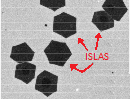
\includegraphics[width=.9\textwidth]{./imagenes/ejemplo1}
			\subcaption{}\label{ejemplo1}
		\end{subfigure}
		\begin{subfigure}[t]{2.5in}
			\centering
			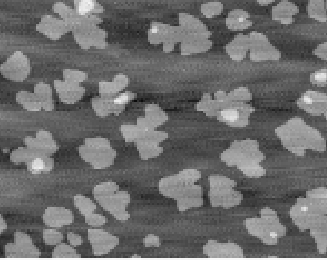
\includegraphics[width=.9\textwidth]{./imagenes/ejemplo2}
			\subcaption{}\label{ejemplo2}
		\end{subfigure}
		\begin{subfigure}[t]{2.5in}
			\centering
			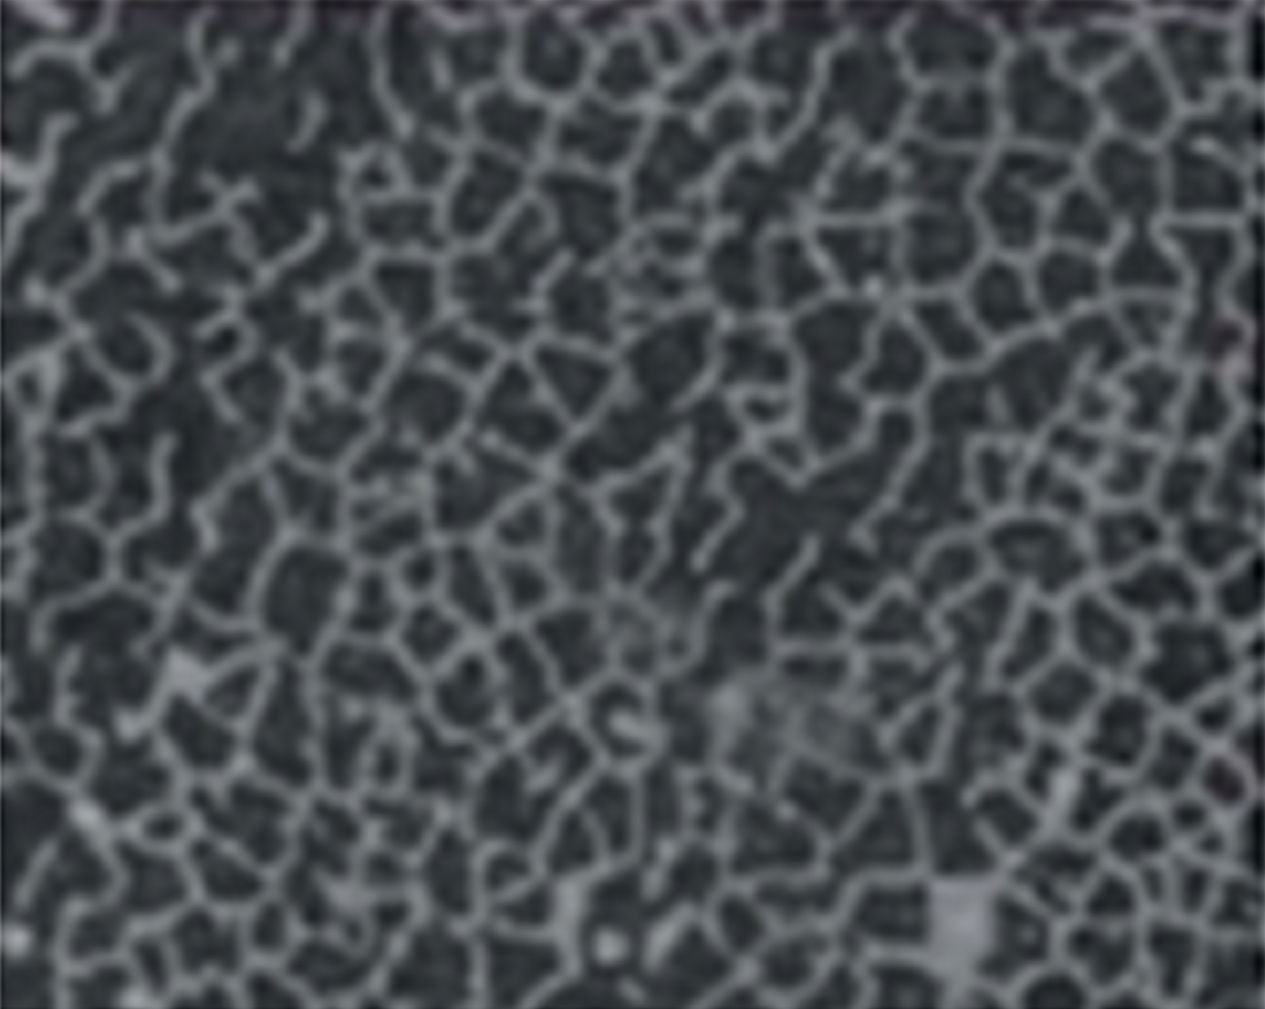
\includegraphics[width=.9\textwidth]{./imagenes/ejemplo3}
			\subcaption{}\label{ejemplo3}
		\end{subfigure}
		\begin{subfigure}[t]{2.5in}
			\centering
			
\includegraphics[width=.9\textwidth]{./imagenes/ejemplo4}
			\subcaption{}\label{ejemplo4}
		\end{subfigure}
	\end{center}
	\caption{Ejemplo de proyecciones en l�minas de materiales sintetizados mediante la deposici�n qu�mica de vapor}	
	\label{ejemploImagenes}
\end{figure}
Las islas puede que est�n muy separadas, como se puede ver en la imagen \ref{ejemplo1} o muy juntas como en la imagen \ref{ejemplo3}. Tambi�n se puede observar que la forma de estas islas no es siempre la misma. Estas caracter�sticas dependen de ciertas variables f�sicas que hacen que el material se <<pegue>> de una determinada manera en la l�mina, dando lugar a estas im�genes abstractas.









\chapter{Conceptos b�sicos}

\section{Definici�n de segmentaci�n}

La segmentaci�n de imagen, tambi�n denominada a veces como \textit{labelling}, es el proceso de dividir la imagen en grupos o regiones contiguas cuyos elementos(p. e. p�xeles o \textit{voxels}) tienen propiedades o caracter�sticas comunes. Estas regiones servir�n para identificar los objetos de la imagen que posteriormente podr�n ser clasificados y etiquetados en base a sus propiedades \cite{terry1}. 

El resultado final de la segmentaci�n de la imagen ser� un conjunto de regiones o segmentos que formar�n la imagen original. Cada uno de los p�xeles de una regi�n tendr� una caracter�stica com�n con los p�xeles de dicha regi�n y una diferencia significativa respecto a p�xeles de otra regi�n, por ello se habr�n agrupado en distinto segmento, ya sea por ejemplo, en el color, la textura o la intensidad. Por lo tanto, se podr�n extraer los segmentos de inter�s de la imagen, es decir, los objetos que �sta contiene.

\section{Evoluci�n de la segmentaci�n}\label{cap:EvoSeg}

Los primeros desarrollos en el �mbito de la segmentaci�n de imagen se remontan a hace 50 a�os. En 1965 se desarroll� un operador para detectar bordes entre diferentes partes de una imagen, conocido como \textit{Roberts operator} o \textit{Roberts Edge Detector}. Este detector fue el primer paso hacia la descomposici�n de im�genes en diferentes segmentos o regiones. En esa misma d�cada tambi�n se propusieron varios detectores de bordes como \textit{Sobel} y \textit{Prewitt edge detectors}. A partir de ah�, comenzaron a surgir diferentes algoritmos y t�cnicas de segmentaci�n. Junto con esto, tambi�n se ampli� el �mbito de estas t�cnicas: de imagen 2D a 3D, de im�genes fijas a im�genes en <<movimiento>> o secuencias de im�genes, de escalas de gris a im�genes a color etc \cite{zhang1}.

A pesar de los a�os de investigaci�n dedicados a estas t�cnicas y el gran n�mero de ellas existentes, la segmentaci�n de imagen sigue siendo un tema de investigaci�n desafiante y no existe a�n un est�ndar de segmentaci�n que funcione bien para cualquier tipo de imagen. Estas t�cnicas est�n en continua evoluci�n y a�n est�n lejos de su madurez. Prueba de ello est� en que muchas conferencias del �mbito de tratamiento de imagen tienen apartados de segmentaci�n, adem�s, el n�mero de art�culos de este �mbito aumenta cada a�o y muchos libros de procesamiento de imagen tienen cap�tulos referidos a la segmentaci�n \cite{zhang1}.

Para que el lector se haga una idea, se ha realizado una b�squeda en el sitio web \textit{ieee explore}\cite{ieee1} con las palabras <<image segmentation>> en varios a�os. Este buscador encuentra art�culos, conferencias, est�ndares, libros, revistas y cursos de aprendizaje relacionados con las palabras introducidas. La figura \ref{regisIEEE} muestra el n�mero de resultados de esa b�squeda desde 1960 hasta 2015. Como se puede observar, el n�mero de resultados aumenta notablemente cada lustro.	
	
\begin{figure}[ht]
	\centering
	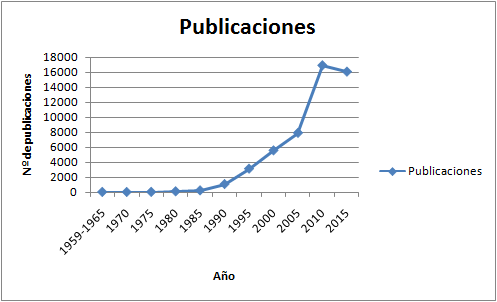
\includegraphics[width=0.9\textwidth]{./imagenes/publicaciones}
	\captionsetup{justification=centering}
	\caption{Resultados de b�squeda en el sitio web \textit{ieee explore} \cite{ieee1} con las palabras <<image segmentation>> }
	\vspace{2 mm}			
	Fuente: \cite{ieee1}
	\label{regisIEEE}
\end{figure}
 
\section{Aplicaciones}

Las aplicaciones de segmentaci�n de im�genes son muchas y muy diversas. Cualquier proceso que requiera la extracci�n de informaci�n de una imagen utilizar�, en cierta medida, una t�cnica de segmentaci�n. A continuaci�n nombraremos algunas de las aplicaciones que se han ido recopilando en la realizaci�n de esta documentaci�n, aunque el n�mero de aplicaciones totales es mucho mayor:

\begin{itemize}
	\item Localizaci�n de mol�culas en im�genes microsc�picas.
	\item Aplicaciones m�dicas.
			\begin{itemize}
				\item Localizaci�n de tumores y otras patolog�as.
			\end{itemize}
	\item Detecci�n de cuerpos para aplicaciones de seguimiento de movimientos como Kinect.
		\begin{itemize}
			\item Operaciones guiadas por ordenador.
		\end{itemize}
	\item Localizaci�n de objetos en im�genes de sat�lite.
	\item Visi�n por computador.
	\item Reconocimientos faciales.
	\item Reconocimiento de plantas
\end{itemize}







\chapter{T�cnicas de segmentaci�n}

\section{Introducci�n}

Hay bastante controversia en cuanto a la clasificaci�n de las diferentes t�cnicas de segmentaci�n, por el gran n�mero de estas t�cnicas existentes, por las diferentes maneras en las que cada una tiene representada la imagen, las diferentes caracter�sticas que utilizan de la imagen etc. Hay trabajos que realizan una clasificaci�n de los algoritmos desde dos puntos de vista diferentes: en funci�n de c�mo puede ser utilizado el algoritmo, es decir, las aplicaciones que pueda tener, y otra en base al algoritmo en s�, fij�ndose en c�mo realiza la segmentaci�n \cite{mc1}. Por otro lado, tambi�n hay otros trabajos que realizan esta clasificaci�n para �mbitos muy concretos \cite[pag. 11]{mc1}.

\textit{Zhang}\cite{zhang1} propone una clasificaci�n m�s clara, creando la divisi�n en dos grupos: a) algoritmos basados en detectar la discontinuidad de las diferentes regiones de la imagen, los llamados \textit{edge-based algorithms} b) basados en detectar la continuidad o la similitud de las regiones, los llamados \textit{region-based algorithms}. Posteriormente hace una subdivisi�n de estos dos grupos en funci�n de la estrategia de procesamiento: los que realizan un procesamiento secuencial, donde el procesamiento de pasos previos se tienen en cuenta en pasos posteriores, y los que realizan un procesamiento paralelo, es decir, decisiones independientes y simult�neas \cite{zhang1}.

\begin{figure}[ht]
	\centering
	\captionsetup{justification=centering}
	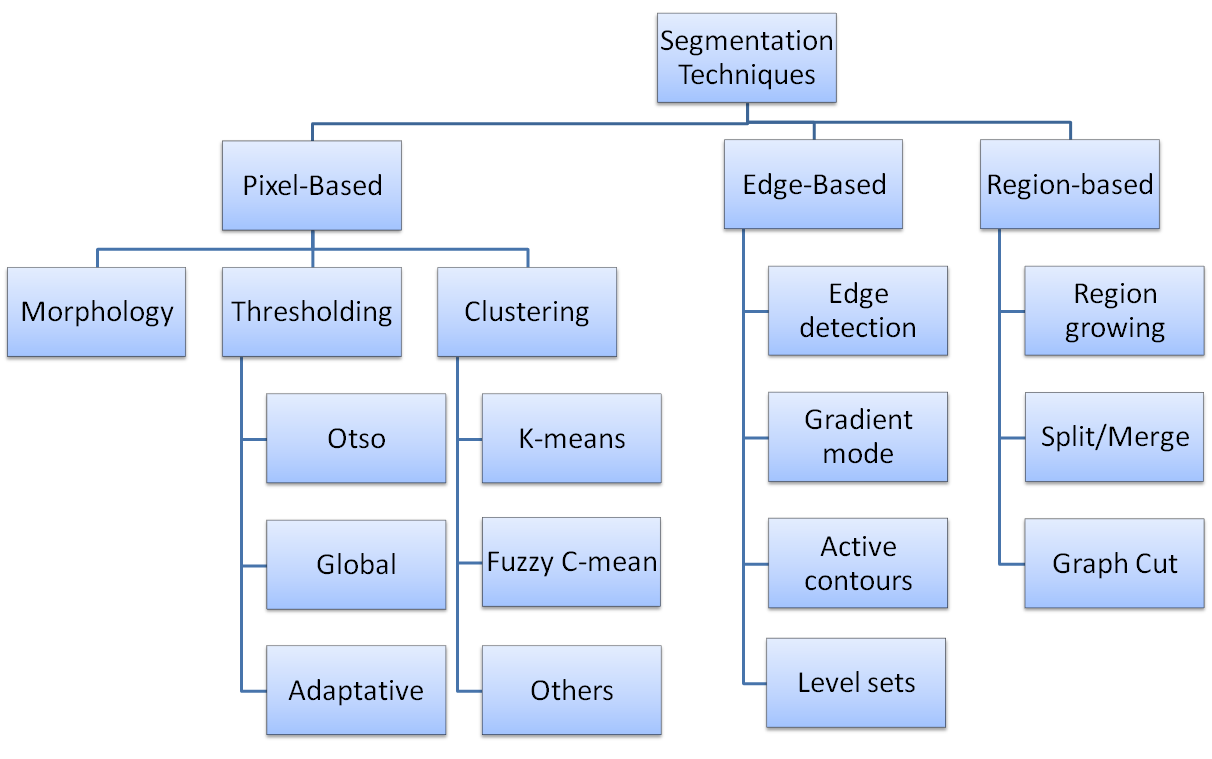
\includegraphics[width=1\textwidth]{./imagenes/tecnicasSegmentacion2}
	\caption{Clasificaci�n de las t�cnicas de segmentaci�n}
	\vspace{2 mm}			
	Fuente: \cite{basa1}
	\label{tecnicasSegmentacion}
\end{figure}

La clasificaci�n elegida tiene varios aspectos en com�n con la �ltima presentada y descrita \cite{basa1}. Se ha preferido esta clasificaci�n al ser clara en cuanto a la divisi�n de las t�cnicas y las caracter�sticas que �stas tienen frente a otras clasificaciones. En la figura  \ref{tecnicasSegmentacion} se muestra el esquema de la clasificaci�n elegida.

\section{Segmentaci�n de imagen basada en el tratamiento de los \textit{p�xeles}}\label{cap:tratPixel}

Este tipo de segmentaci�n consiste en dividir la imagen en segmentos o  conjuntos de p�xeles (conocidos como <<superp�xeles>>). Cada p�xel de la imagen ser� tratado y agrupado en funci�n de sus caracter�sticas. Existen varios subgrupos dentro de esta clasificaci�n: \textit{Thresholding},o <<M�todo del valor umbral>> en castellano, y \textit{Clustering}, o algoritmos de agrupamiento en castellano, entre otros.

\subsection{Thresholding}

Este tipo de segmentaci�n es la m�s simple de todas y se basa en clasificar los p�xeles en dos grupos en funci�n de la intensidad de �stos: los que superan la intensidad umbral definida y los que no la superan. El resultado de esta segmentaci�n ser�a una imagen binaria (v�ase la comparaci�n de las figuras \ref{thresholding1} y \ref{thresholding2}). 

Esta t�cnica puede ser definida como:

\

Para una imagen NxM :

for $i = 1,2, ... , N \ $and$ \ j = 1,2, ... , M $
\begin{equation}
 f(n) = \left\{ 
\begin{array}{l l}
1 & \quad \mathrm{si \ I(i,j) \ge T}\\
0 & \quad \mathrm{si \ I(i,j) <\ T}
\end{array} \right. 
\end{equation}
donde $I(i,j)$ es el valor del p�xel de la posici�n i,j de la imagen.

Tambi�n existe la posibilidad de definir varias intensidades umbrales (v�ase la comparaci�n de las figuras \ref{thresholding3} y \ref{thresholding4}), con el fin de particionar la imagen en m�s segmentos. En s�, se podr�n definir tantos umbrales como niveles de gris contiene la imagen, aunque habr� que buscar un buen equilibrio. 

La ventaja de este tipo de segmentaci�n es que es relativamente sencilla comparada con otros tipos de segmentaci�n m�s avanzada como \textit{watershed} o \textit{level set}. Aun as�, esta segmentaci�n funciona bien cuando el fondo y los objetos siguen una distribuci�n bimodal, es decir, que hay una diferencia <<notable>> entre las dos partes. Com�nmente esta caracter�stica no se da en todas las im�genes, por lo que no tendr� buenos resultados en las que el fondo no se distinga bien de los objetos \cite{basa1}. Adem�s, esta segmentaci�n tampoco se comporta bien con im�genes que tienen una iluminaci�n gradiente grande (v�ase la comparaci�n de las figuras \ref{thresholding5} y \ref{thresholding6}). Aunque es verdad que para ello tambi�n existen varias mejoras que hacen que la segmentaci�n se <<adapte>> para conseguir mejores resultados.

En la figura \ref{tecnicasSegmentacion} se muestran varias subclases de \textit{thresholding}. Aunque no se explicar�n en profundidad conviene saber que hay varias maneras de realizar esta segmentaci�n. Primeramente se nombra el m�todo de Otso, \textit{Otsu's method} en ingl�s, que adapta el umbral en funci�n de la dispersi�n de los niveles de gris. El segundo m�todo, el \textit{Global}, es el m�s simple y el que hemos estado explicando hasta ahora. Y por �ltimo, el m�todo \textit{Adaptative}, mencionado anteriormente, que se adapta a la intensidad de la imagen.

\begin{figure}[H]
	\centering
	\captionsetup{justification=centering}
	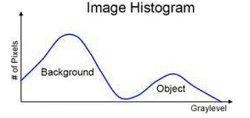
\includegraphics[width=.65\textwidth]{./imagenes/imageHistogram}
	\caption{Histograma que muestra tres aparentes segmentos de la imagen con dos umbrales}
	\vspace{2 mm}					
	Fuente: \cite{basa1}	
	\label{imageHistogram}
\end{figure}

Las figuras \ref{thresHold1}, \ref{thresHold2} y \ref{thresHold3} muestran varios ejemplos de segmentaci�n utilizando \textit{thresholding}.
\vspace{-2 mm}			
\begin{figure}[H]
	\captionsetup{justification=centering}
	\centering
	\begin{subfigure}[t]{2.5in}
		\centering
		\includegraphics[width=.9\textwidth]{./imagenes/thresholding1}
		\subcaption{Imagen original}\label{thresholding1}		
	\end{subfigure}
	\begin{subfigure}[t]{2.5in}
		\centering
		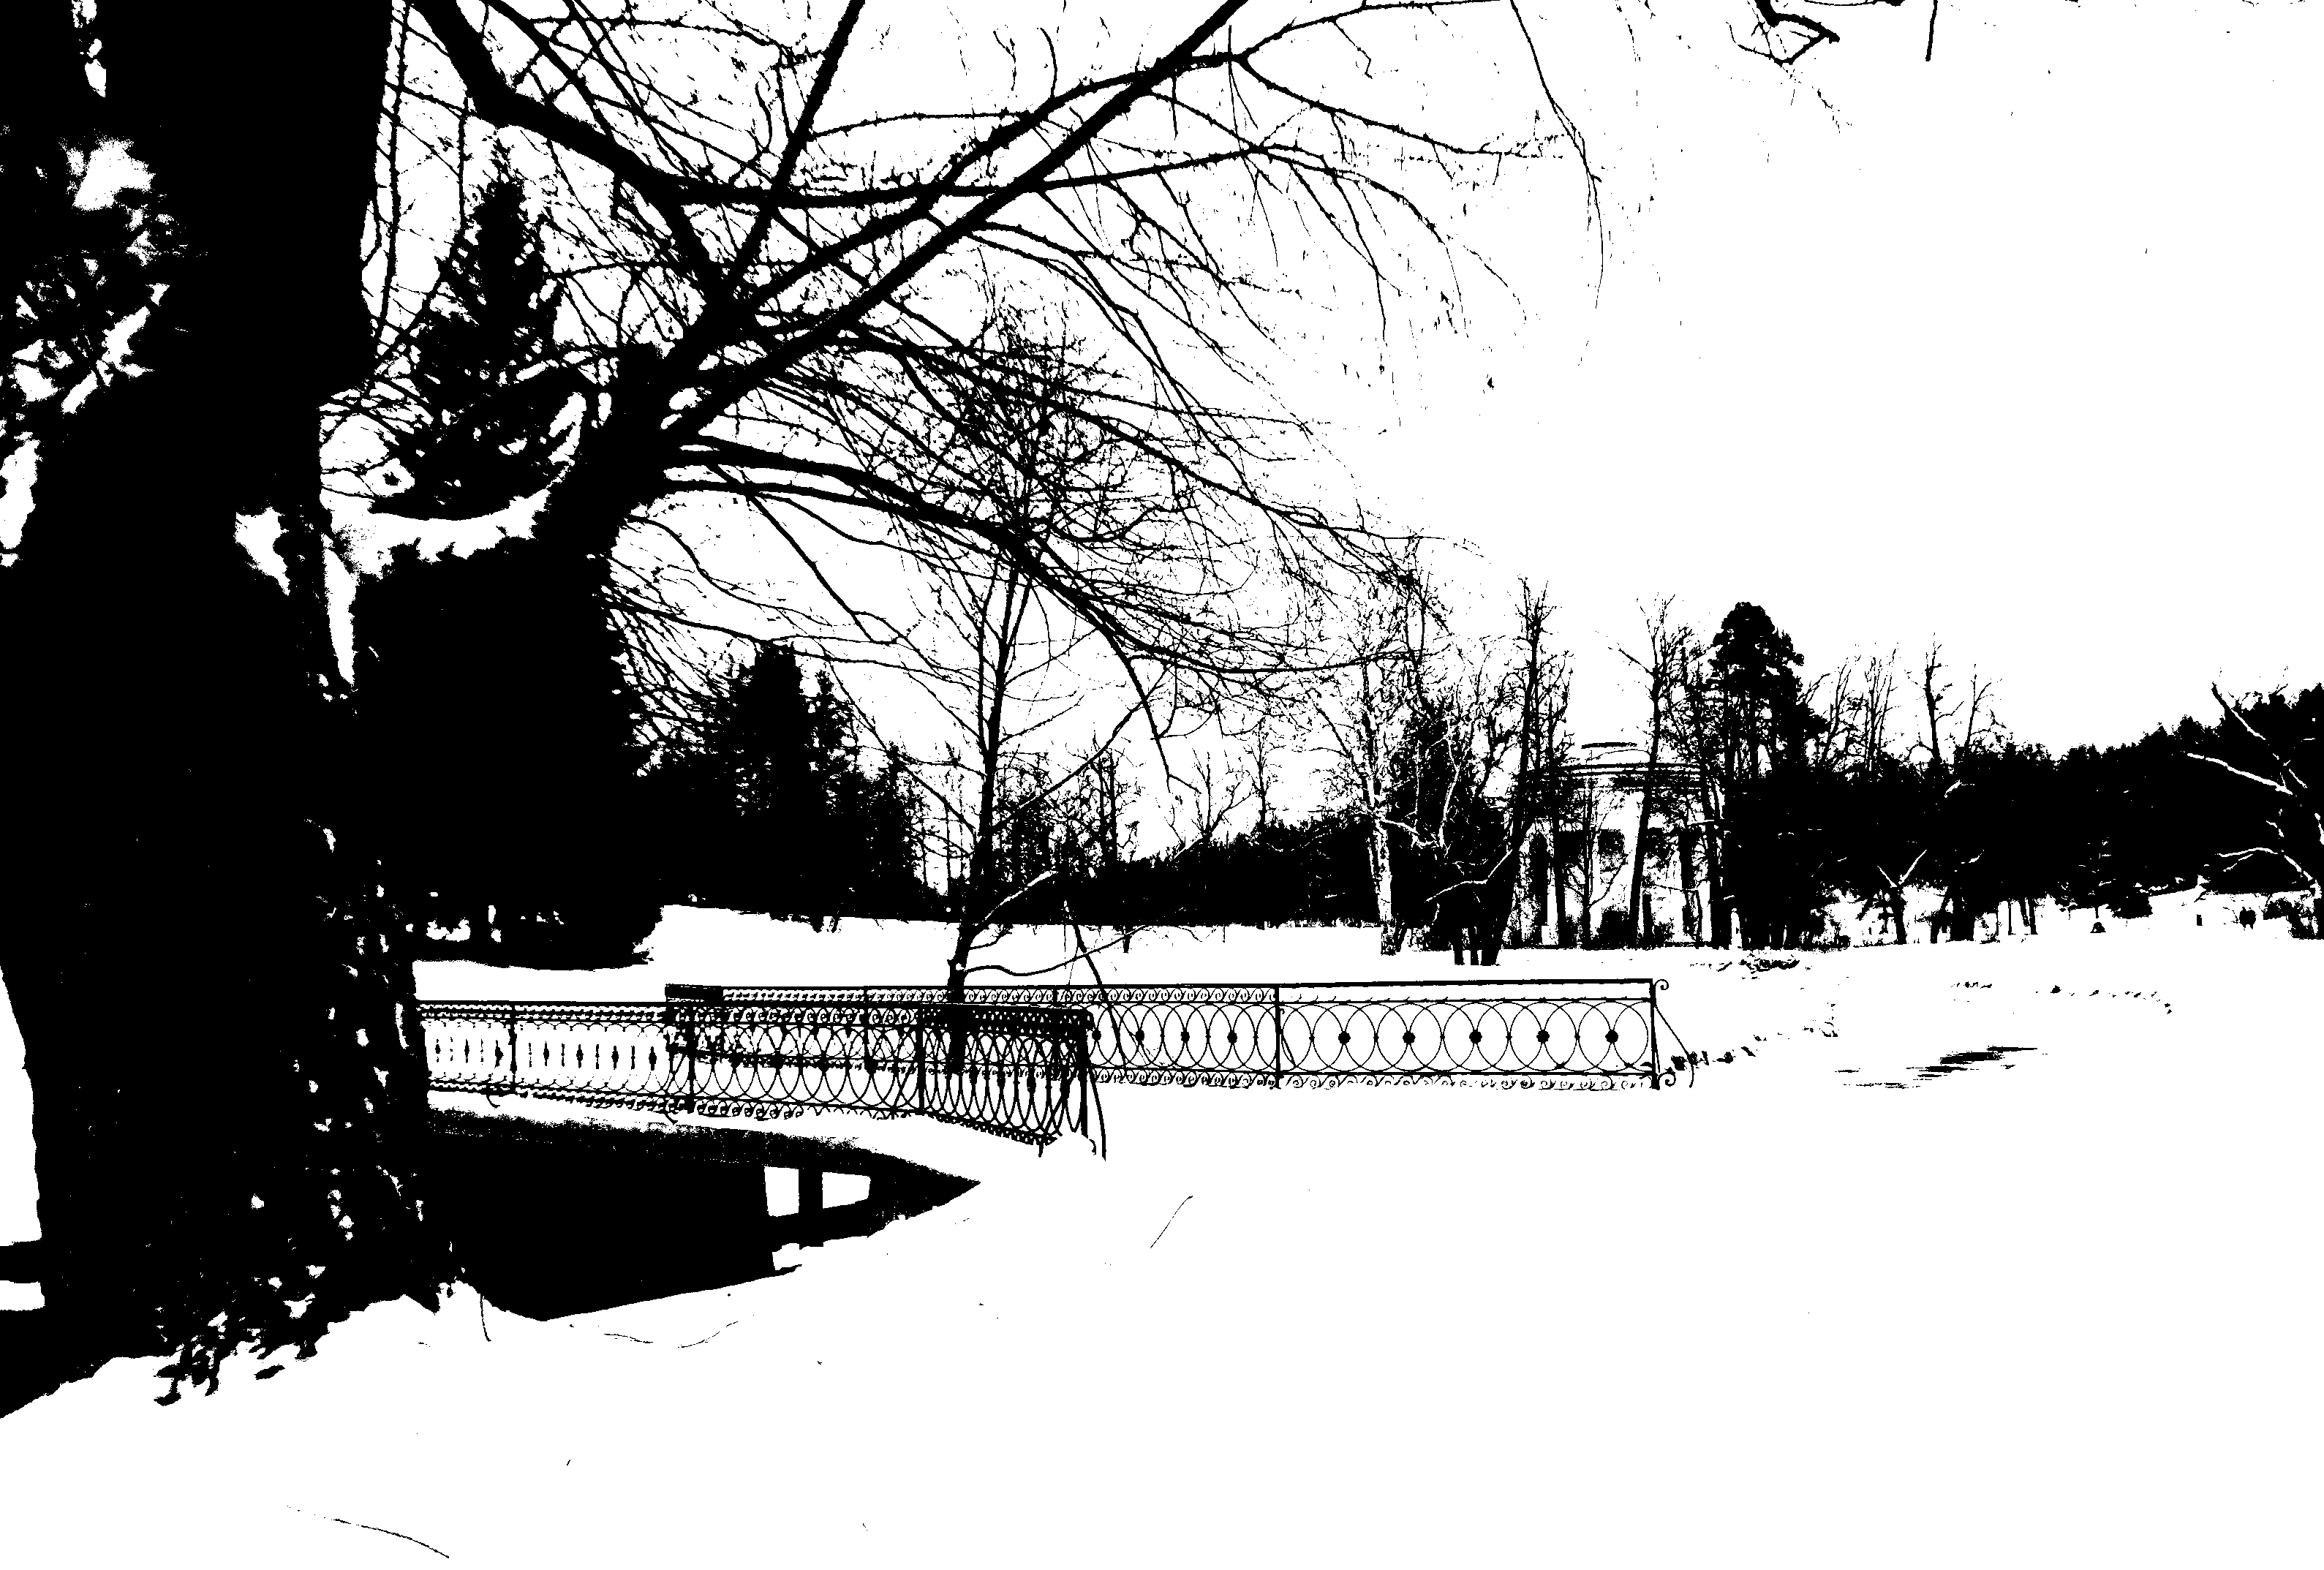
\includegraphics[width=.9\textwidth]{./imagenes/thresholding2}
		\subcaption{Imagen segmentada}\label{thresholding2}
	\end{subfigure}
	\caption{Segmentaci�n con \textit{thresholding}}	
	\vspace{2 mm}			
	Fuente: commons.wikimedia.org	
	\label{thresHold1}
\end{figure}	
\begin{figure}[H]	
	\captionsetup{justification=centering}	
	\centering	
	\begin{subfigure}[t]{2.5in}
		\centering
		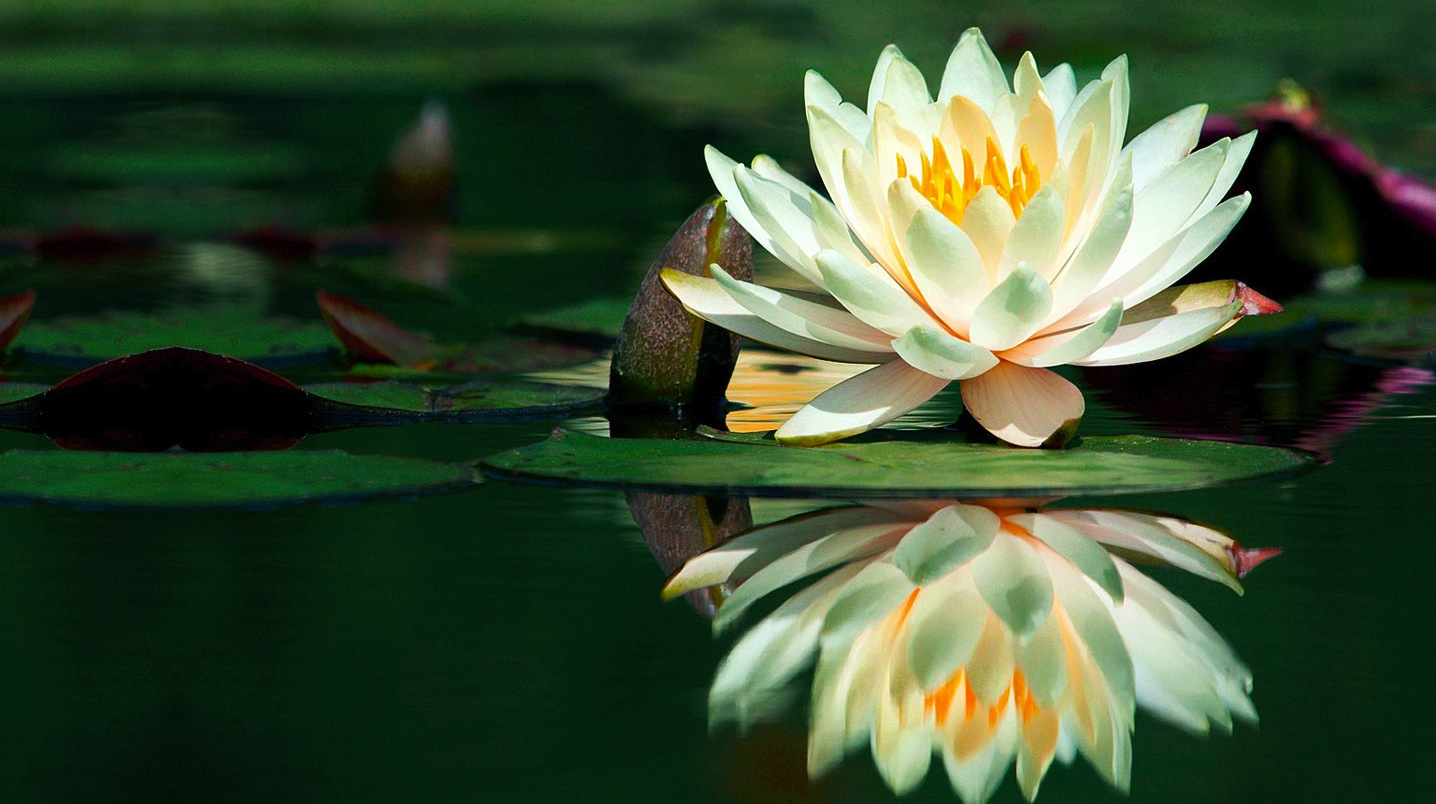
\includegraphics[width=.9\textwidth]{./imagenes/thresholding3}
		\subcaption{Imagen original}\label{thresholding3}
	\end{subfigure}
	\begin{subfigure}[t]{2.5in}
		\centering
		
\includegraphics[width=.9\textwidth]{./imagenes/thresholding4}
		\subcaption{Imagen segmentada}\label{thresholding4}
	\end{subfigure}
	\caption{Segmentaci�n con \textit{thresholding} con varios umbrales}
	\vspace{2 mm}			
	Fuente: \textit{rosavallsformacio.tv} y \textit{photo-kako.com} para la realizaci�n de la segmentaci�n
	\label{thresHold2}
\end{figure}	
\begin{figure}[H]
	\centering
	\captionsetup{justification=centering}
	\begin{subfigure}[t]{2.5in}
		\centering
		
\includegraphics[width=.7\textwidth]{./imagenes/thresholding5}
		\subcaption{Imagen original}\label{thresholding5}
	\end{subfigure}
	\begin{subfigure}[t]{2.5in}
		\centering
		
\includegraphics[width=.7\textwidth]{./imagenes/thresholding6}
		\subcaption{Imagen segmentada}\label{thresholding6}
	\end{subfigure}
	\caption{Segmentaci�n con \textit{thresholding} en imagen con iluminaci�n gradiente}
	\vspace{2 mm}			
	Fuente: \textit{homepages.inf.ed.ac.uk/rbf/HIPR2/}
	\label{thresHold3}
\end{figure}


\subsection{Clustering}

Junto con la t�cnica de \textit{thresholding} el \textit{clustering} es la t�cnica de segmentaci�n m�s utilizada. En general esta t�cnica divide los puntos en varios \textit{clusters} o grupos en funci�n de la distancia entre ellos. En este caso concreto, los puntos ser�n los p�xeles de la imagen y la distancia entre ellos estar� relacionada con la intensidad, color y textura, pudiendo combinar varios de estos factores. 

Los algoritmos de \textit{clustering} se pueden dividir entre jer�rquicos y particionales, donde la principal diferencia entre los dos est� en el modo en que se construyen los grupos. Los algoritmos jer�rquicos suelen ser m�s precisos, sin embargo, no valen para una cantidad de datos grande como en una imagen ya que el coste computacional es muy elevado. Por lo tanto, la opci�n escogida suele ser el \textit{clustering} particional. No obstante, esta t�cnica tiene varias desventajas \cite{oli1}:

\begin{enumerate}
	\item Generalmente es necesario saber previamente el n�mero de \textit{clusters} que hay en la imagen. 
	\item No utilizan informaci�n espacial inherente a la imagen.
	\item En algunos algoritmos de clustering, como el K-means que se explicar� a continuaci�n, no se asegura un resultado �ptimo, ya que distintas inicializaciones dan diferentes resultados.
\end{enumerate} 

En la clasificaci�n presentada en la figura \ref{tecnicasSegmentacion} se muestran varias subclases de la t�cnica de \textit{clustering} que corresponden a diferentes algoritmos de creaci�n de \textit{clusters}. El algoritmo \textit{Fuzzy C-Means} agrupa los p�xeles utilizando la l�gica difusa, donde cada p�xel tendr� un grado de pertenencia a todos los \textit{clusters}. En general, hay muchos tipos de t�cnicas de clustering por lo que las t�cnicas restantes se agrupar�n en la secci�n de \textit{Others} de la figura \ref{tecnicasSegmentacion}. El algoritmo K-means es el m�s utilizado (v�ase ejemplos de su segmentaci�n en las figuras \ref{clusteringTotal1} y \ref{clusteringTotal2}). Una descripci�n de su modo de funcionamiento a grandes rasgos ser�a:

\begin{enumerate}
 \item Se asignan \textit{K} primeros p�xeles como centroides.
 \item Se agrupan los p�xeles, restantes con los centroides definidos en funci�n de la distancia con estos.
 \item Se calculan los nuevos \textit{K} centroides como los baricentros de los \textit{K} conglomerados obtenidos.
 \item Se alternan los pasos 2 y 3 hasta que se alcance un determinado criterio de convergencia (m�xima variaci�n de centroides, por ejemplo).
\end{enumerate}

\begin{figure}[H]
	\captionsetup{justification=centering}
	\centering
	\begin{subfigure}[t]{2.5in}
		\centering
		\includegraphics[width=.9\textwidth]{./imagenes/clustering1}
		\subcaption{Imagen original}\label{clustering1}
	\end{subfigure}
	\begin{subfigure}[t]{2.5in}
		\centering
		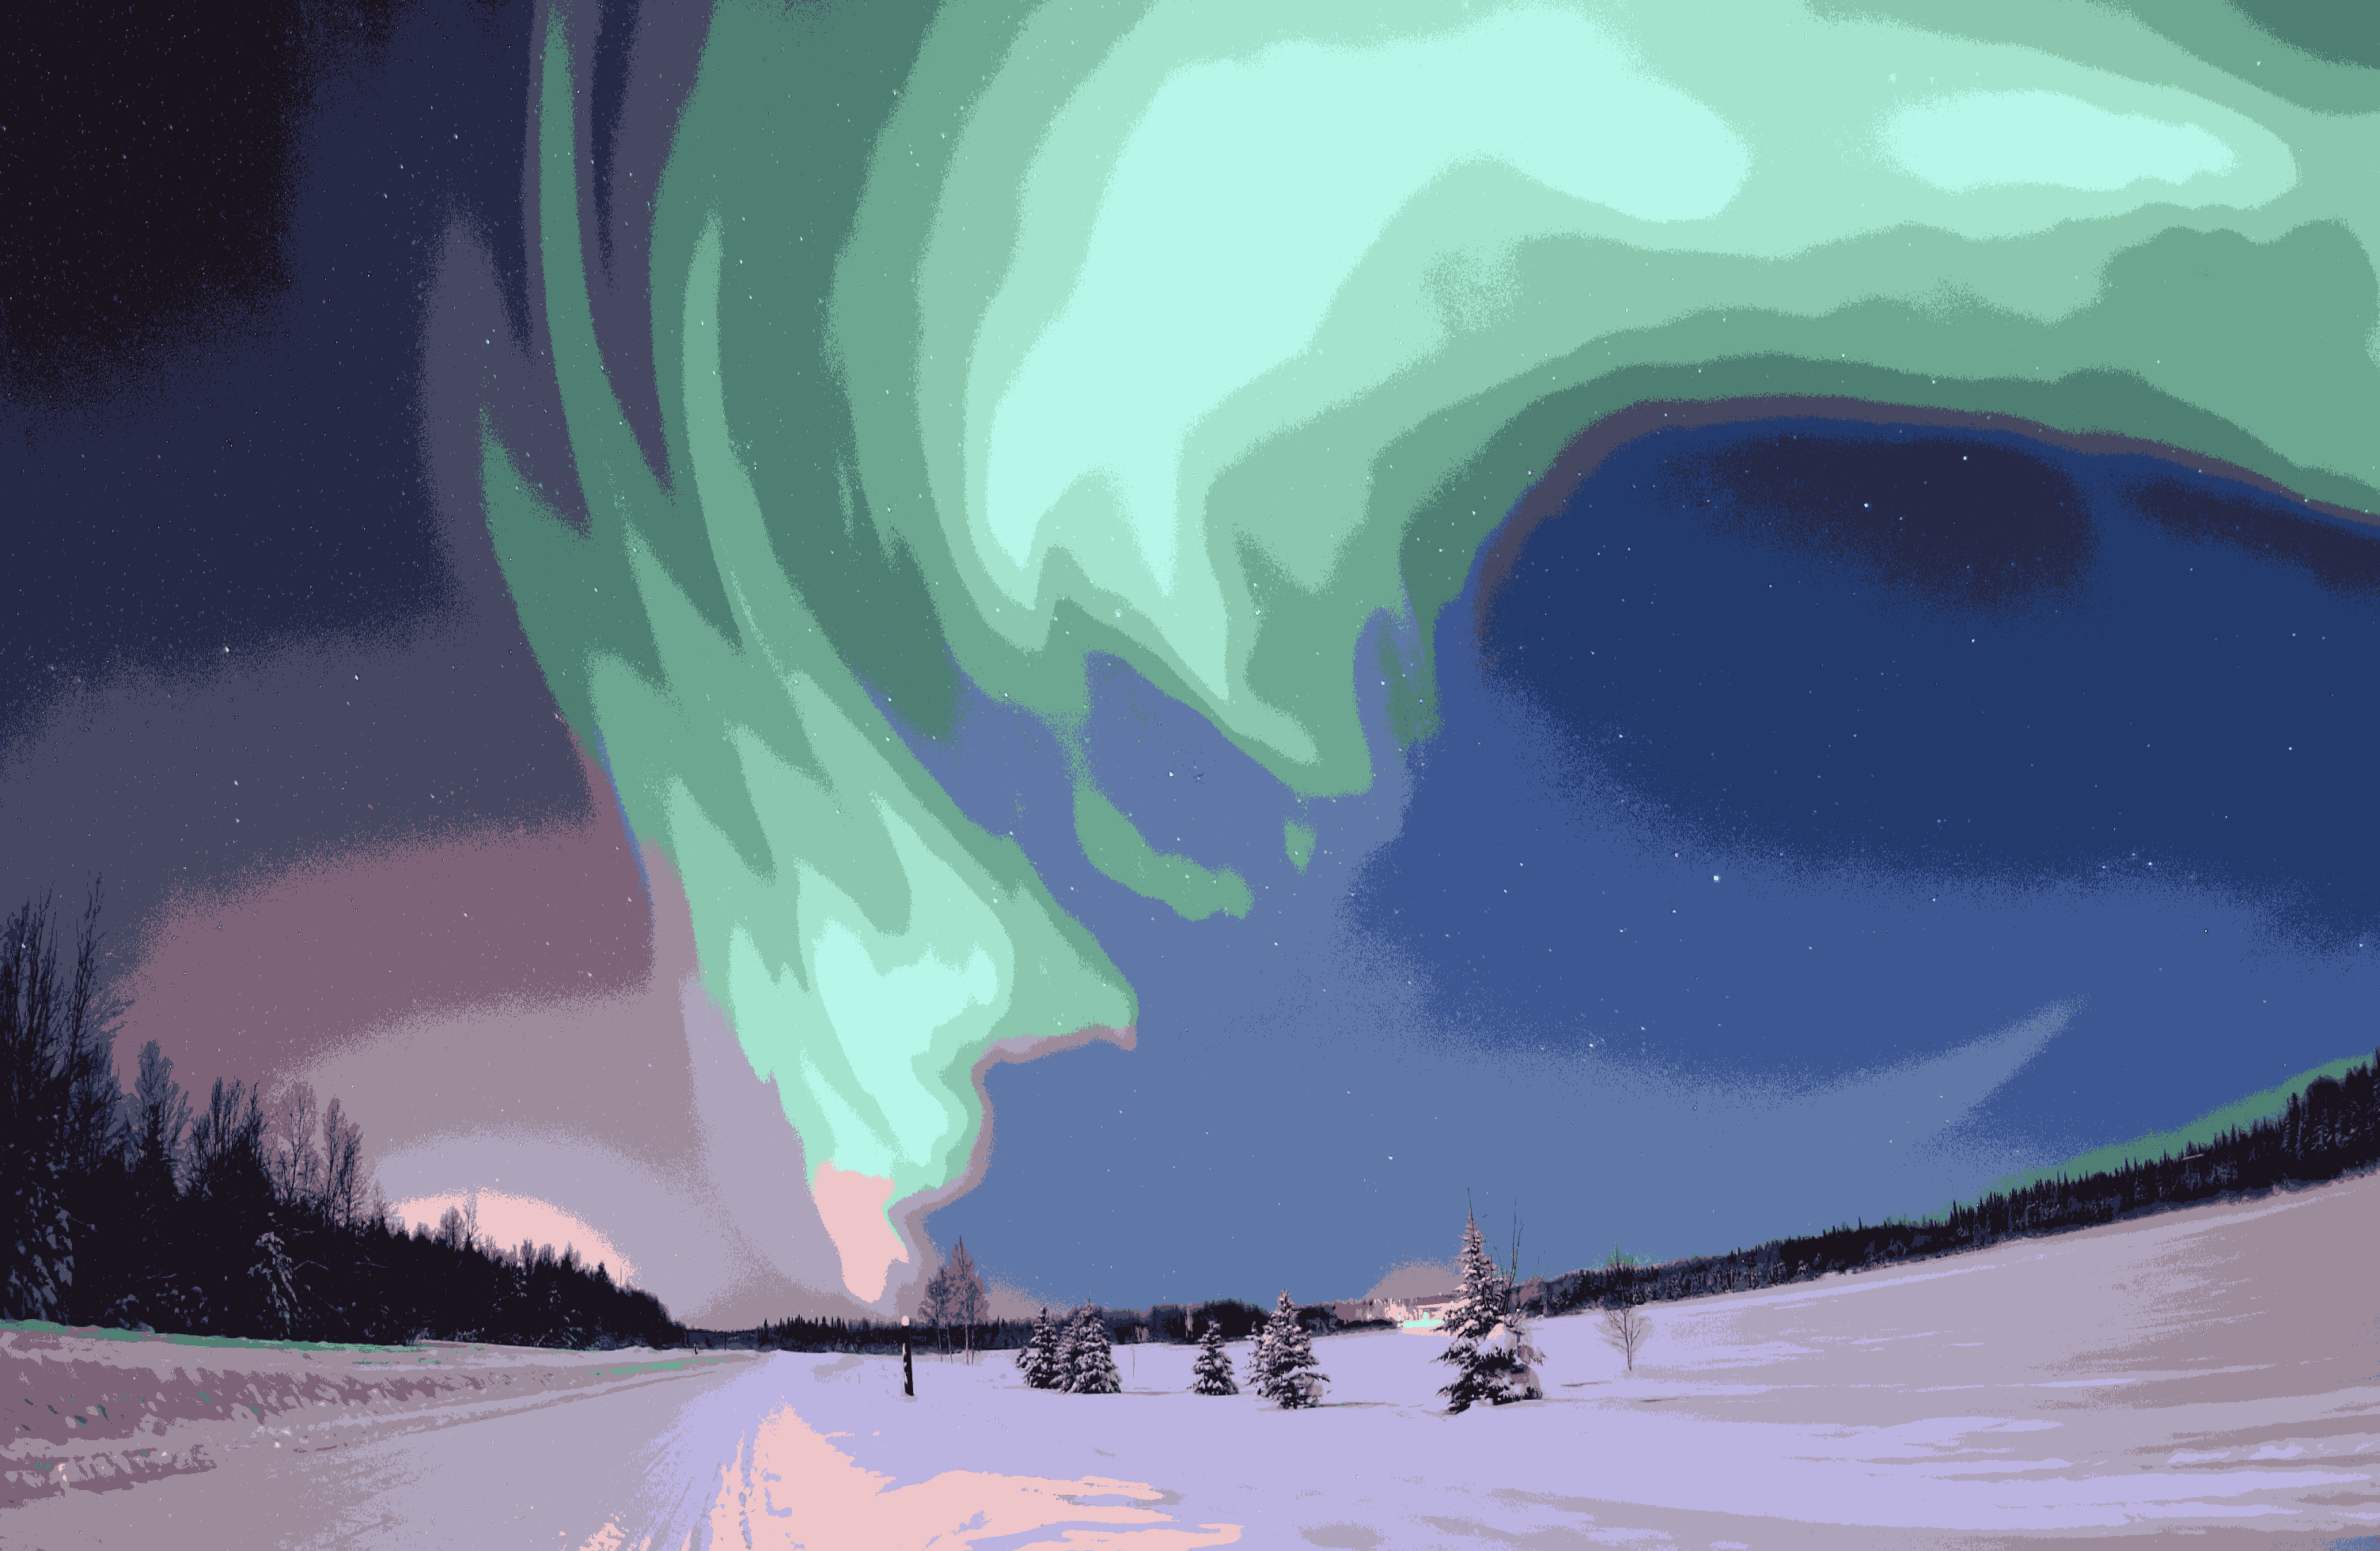
\includegraphics[width=.9\textwidth]{./imagenes/clustering2}
		\subcaption{Imagen segmentada}\label{clustering2}
	\end{subfigure}
	\caption{Segmentaci�n utilizando K-means con K=16}
	\vspace{2 mm}
	\label{clusteringTotal1}			
	Fuente: commons.wikipedia.org
\end{figure}
\begin{figure}[H]
	\centering
	\captionsetup{justification=centering}
	\begin{subfigure}[t]{2.5in}
		\centering
		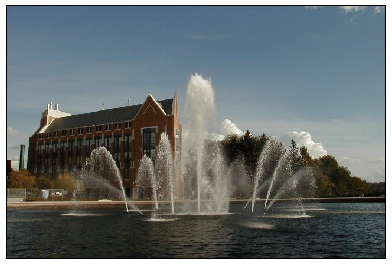
\includegraphics[width=1\textwidth]{./imagenes/clustering3}
		\subcaption{Imagen original}\label{clustering3}
	\end{subfigure}
	\begin{subfigure}[t]{2.5in}
		\centering
		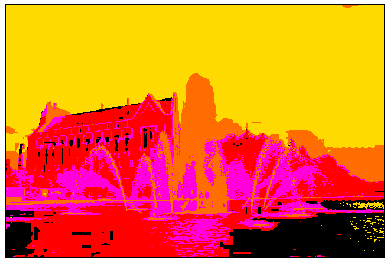
\includegraphics[width=1\textwidth]{./imagenes/clustering4}
		\subcaption{Imagen segmentada}\label{clustering4}
	\end{subfigure}
	\caption{Segmentaci�n utilizando K-means con K=6}
	\vspace{2 mm}
	\label{clusteringTotal2}			
	Fuente: \textit{imagedatabase.cs.washington.edu/demo/kmcluster/}
\end{figure}

\subsection{Morphology}

La t�cnica de la morfolog�a, o \textit{morphology} en ingl�s, se clasificar�a dentro de las t�cnicas basadas en el tratamiento de los p�xeles. Hay varios m�todos de morfolog�a y se basan en una m�scara llamada \textit{structuring element} para investigar cada p�xel. El valor de cada p�xel est� determinado por el de sus vecinos que pertenecen a esa m�scara. Los m�todos m�s simples de esta t�cnica son la dilataci�n y la erosi�n. Para una imagen binaria, la dilataci�n convierte en uno todos los p�xeles de la m�scara si los p�xeles <<debajo>> del p�xel central son ceros como se muestra en la imagen \ref{morphology1}. La erosi�n es el caso contrario, es decir, convierte en ceros todos los elementos de la m�scara si esta contiene alg�n elemento que sea cero. La combinaci�n de estas simples operaciones junto con otras como el complemento, la uni�n y la intersecci�n, pueden utilizarse para realizar operaciones m�s avanzadas y complejas. 
 
\begin{figure}[ht]
	\centering
	\captionsetup{justification=centering}
	\begin{subfigure}[t]{2.5in}
		\centering
		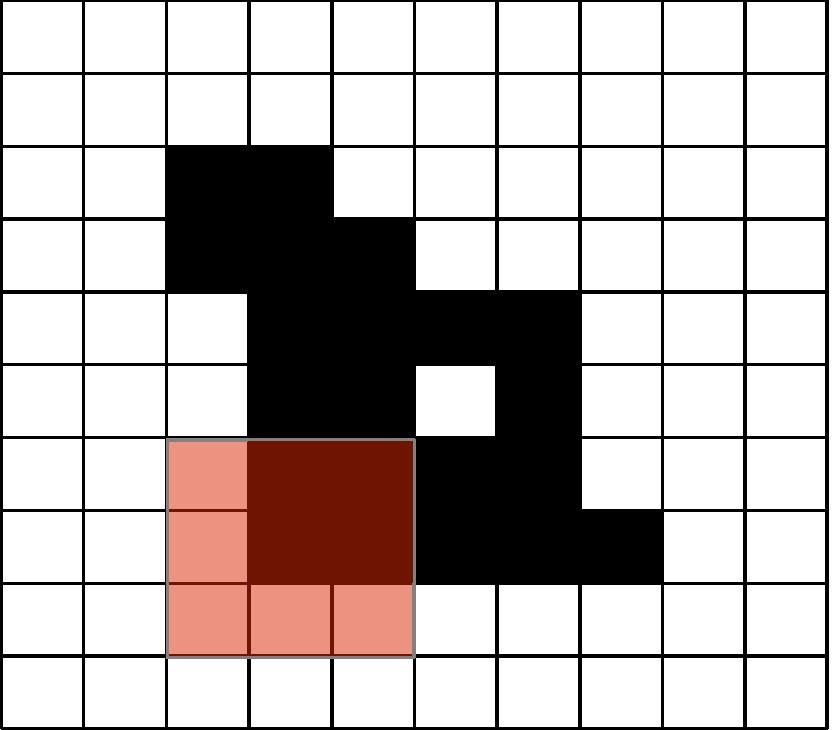
\includegraphics[width=.8\textwidth]{./imagenes/morphology1-1}
		\subcaption{Imagen sin tratar}\label{morphology1.1}
	\end{subfigure}	
	\begin{subfigure}[t]{2.5in}
		\centering
		
\includegraphics[width=.8\textwidth]{./imagenes/morphology1-2}
		\subcaption{Resultado de la dilataci�n}\label{morphology1.2}
	\end{subfigure}
	\caption{Ejemplo de dilataci�n de la t�cnica de morfolog�a}
	\vspace{2 mm}
	Fuente: \cite{eri2015}
	\label{morphology1}
\end{figure}

\section{Segmentaci�n de imagen basada en la detecci�n de bordes}

Este tipo de segmentaci�n consiste en encontrar los bordes de los objetos contenidos en la imagen con el fin de poder dividir la imagen en funci�n de los bordes encontrados. Los detectores de bordes tradicionales suelen utilizar los operadores diferenciales de detecci�n de bordes comentados en \ref{cap:EvoSeg}, es decir, los operadores \textit{Sobel}, \textit{Roberts} y \textit{Prewitt edge detectors} que est�n basados en el gradiente de la funci�n de intensidad de una imagen. Normalmente los bordes suelen detectarse en las intersecciones de dos regiones de la imagen que tienen diferentes intensidades.

La ventaja de este tipo de segmentaci�n frente a la basada en el tratamiento de p�xeles es que, aparte de hacer la divisi�n de las diferentes regiones, sabremos exactamente d�nde se encuentran los bordes de �stas, siendo �til para poder extraerlas y poder tratarlas individualmente. Por lo tanto, esta t�cnica funcionar� mejor cuando la diferencia entre las regiones tenga buena calidad. Una de las posibles <<desventajas>> puede ser que la detecci�n de muchos bordes dificulte la extracci�n de las regiones de inter�s.

Existen varios subgrupos dentro de esta clasificaci�n: \textit{Edge detection} o <<Detecci�n de bordes>> en castellano, t�cnicas que tienen que ver con el gradiente de la imagen \textit{Gradient mode}, \textit{Active contours} o <<Contornos activos>> y \textit{level sets} o t�cnicas del <<Conjunto de nivel>>.

\subsection{Detecci�n de borde usando gradientes}

En la figura \ref{tecnicasSegmentacion} se diferencian las dos primeras clasificaciones \textit{Edge detection} y \textit{Gradient mode} pero al estar directamente relacionadas se ha decidido explicarlas en conjunto. 

Las t�cnicas cl�sicas de detecci�n de bordes se basan en encontrar la derivada respecto a los ejes que forman la imagen, o dicho de otro modo, el gradiente. El gradiente de un punto de una funci�n escalar, representado con $\nabla$, se representa en forma vectorial. Este vector indica la direcci�n en la cual la funci�n varia m�s r�pidamente y su m�dulo representa el ritmo de variaci�n de la funci�n en la direcci�n de dicho vector. Este m�dulo se utilizar� para determinar si un punto es borde o no, en funci�n de si supera un valor umbral dado. Para encontrar la m�xima variaci�n en ese punto se deben de hacer las derivadas parciales respecto a cada eje y coger el m�ximo valor de �stas. En general el gradiente se suele aproximar con la f�rmula\protect\footnotemark \footnotetext{V�lida para una imagen de dos dimensiones. En caso de tener tres dimensiones la f�rmula ser�a $|G| \approx |G_x| + |G_y| + |G_z| $ }$|G| \approx |G_x| + |G_y| $  que es mucho m�s simple de implementar en la pr�ctica. Vali�ndonos de esto, se desarrollaron los primeros operadores diferenciales ya comentados  \textit{Sobel}, \textit{Roberts} y \textit{Prewitt edge detectors} (v�ase un ejemplo de cada segmentaci�n en la figura \ref{prewittTable2}). Estos operadores no son m�s que m�scaras aplicadas al p�xel a tratar y a cierta vecindad de �ste para calcular una aproximaci�n a dichas derivadas $G_x$ y $G_y$. De ah� el nombrarlos como <<operadores>>.

\

\subsubsection{$\blacksquare$ \quad Roberts operator}

Este operador es el m�s simple de los tres mencionados y aproxima las derivadas tomando la diferencia de dos valores contiguos. La gran desventaja de este operador es que es muy sensible al ruido al tratar pocos vecinos y s�lo permite marcar los puntos del borde pero no su orientaci�n. A pesar de todo ello, es un operador que computacionalmente es poco costoso debido a su simpleza y que trabaja bien con im�genes binarias. V�ase las m�scaras utilizadas por esta t�cnica presentada en la tabla \ref{robetsTable}. 

\begin{table}[H]
	\parbox{.65\linewidth}{
		\centering
		\begin{tabular}{|c|c|}
			\hline
			+1 & 0 \\ \hline
			0  & -1 \\ \hline
		\end{tabular}
		\caption*{$G_x$}
	}
	\hspace*{-50mm}
	\parbox{.65\linewidth}{
		\centering
		\begin{tabular}{|c|c|}
			\hline
			0 & +1 \\ \hline
			-1  & 0 \\ \hline
		\end{tabular}
		\caption*{$G_y$}
	}
	\captionsetup{justification=centering}
	\caption{M�scaras utilizadas por el operador de Roberts de tama�o 2x2}
	\label{robetsTable}
\end{table}

\subsubsection{$\blacksquare$ \quad Sobel operator}

Este operador utiliza una m�scara m�s grande que el \textit{Roberts operator}, 3x3, por lo que implicar� a m�s vecinos. Enfatiza m�s los p�xeles de alrededor del centro. La ventaja de este operador es que es menos sensible al ruido, detecta muy bien los bordes horizontales y verticales y adem�s proporciona un suavizado. Las desventaja de este operador es que computacionalmente es m�s costoso, no tiene buena detecci�n de bordes diagonales y no da informaci�n sobre la orientaci�n del borde. V�ase las m�scaras utilizadas por esta t�cnica presentada en la tabla \ref{sobelTable}.
\begin{table}[H]
	\parbox{.45\linewidth}{
	\centering
		\begin{tabular}{|c|c|c|}
			\hline
			-1 & 0 & +1 \\ \hline
			-2 & 0 & +2 \\ \hline
			-1 & 0 & +1 \\ \hline
		\end{tabular}
	\caption*{$G_x$}
	}
	\parbox{.45\linewidth}{
	\centering
		\begin{tabular}{|c|c|c|}
			\hline
			+1 & +2 & +1 \\ \hline
			0  & 0  & 0  \\ \hline
			-1 & -2 & -1 \\ \hline
		\end{tabular}
		\caption*{$G_y$}
	}
	\captionsetup{justification=centering}
	\caption{M�scaras utilizadas por el operador de Sobel de tama�o 3x3}
	\label{sobelTable}
\end{table}

\subsubsection{$\blacksquare$ \quad Prewitt operator}

Este operador es parecido al operador de Sobel pero este no enfatiza los p�xeles cercanos al centro y los coeficientes son diferentes. Las ventajas son que aumenta la respuesta a los bordes diagonales poni�ndole peso a p�xeles vecinos que antes no ten�an, tiene poca sensibilidad la ruido y proporciona la magnitud y orientaci�n del borde (hasta 8 direcciones). V�ase las m�scaras utilizadas por esta t�cnica presentada en las tablas \ref{prewittTable1} y \ref{prewittTable2}.
 \begin{table}[H]
 	\parbox{.45\linewidth}{
 		\centering
		\begin{tabular}{|c|c|c|}
			\hline
			-1 & +1 & +1 \\ \hline
			-1 & -2 & +2 \\ \hline
			-1 & +1 & +1 \\ \hline
		\end{tabular}
 		\caption*{0}
 	}
 	\parbox{.45\linewidth}{
 		\centering
			\begin{tabular}{|c|c|c|}
				\hline
				+1 & +1 & +1 \\ \hline
				-1 & -2 & +1 \\ \hline
				-1 & +1 & +1 \\ \hline
			\end{tabular}
 		\caption*{45}
 	}
	\captionsetup{justification=centering}
 	\caption{M�scaras utilizadas por el operador de Prewitt de tama�o 3x3}
	\label{prewittTable1}
 \end{table}

\begin{figure}[H]
	\captionsetup{justification=centering}
	\begin{subfigure}[t]{2.5in}
		\centering
		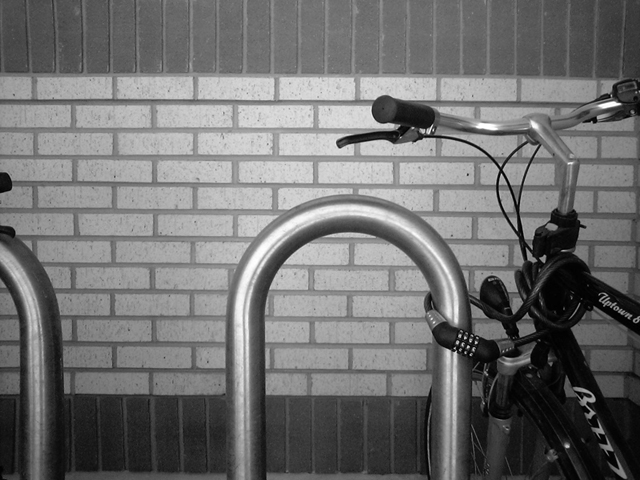
\includegraphics[width=.9\textwidth]{./imagenes/operator0}
		\subcaption{Imagen original}\label{operator0}
	\end{subfigure}
	\begin{subfigure}[t]{2.5in}
		\centering
		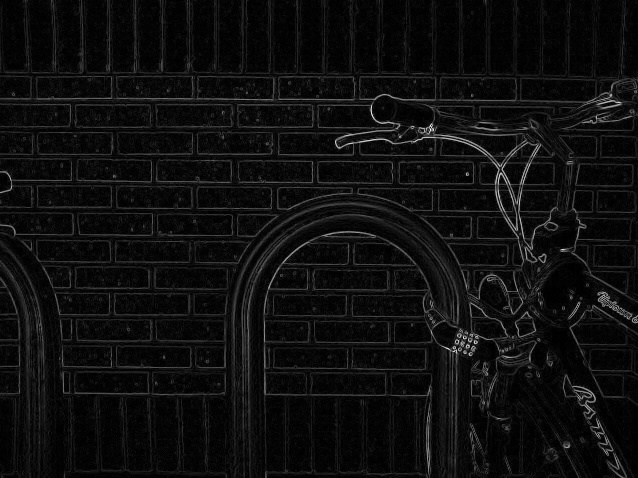
\includegraphics[width=.9\textwidth]{./imagenes/operator1}
		\subcaption{Resultado de \textit{Roberts operator}}\label{operator1}
	\end{subfigure}
	
	\begin{subfigure}[t]{2.5in}
		\centering
		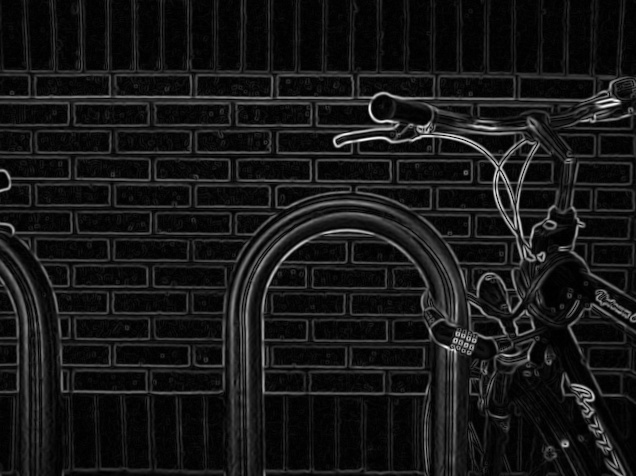
\includegraphics[width=.9\textwidth]{./imagenes/operator2}
		\subcaption{Resultado de \textit{Sovel operator}}\label{operator2}
	\end{subfigure}
	\begin{subfigure}[t]{2.5in}
		\centering
		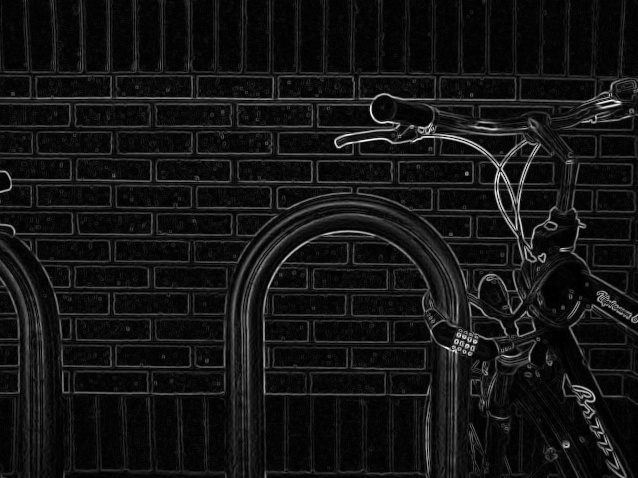
\includegraphics[width=.9\textwidth]{./imagenes/operator3}
		\subcaption{Resultado de \textit{Prewitt operator}}\label{operator3}
	\end{subfigure}
	\caption{Detecci�n de bordes con el uso de los operadores}
	\vspace{2 mm}
	\centering
	\label{prewittTable2}
	Fuente: commons.wikipedia.org
\end{figure}

\subsection{Active Contours}\label{cap:actContour}

Desde que fueron introducidos por Kass y colaboradores en 1988 \cite{kass1}, los contornos activos o m�s com�nmente nombrados como \textit{Snakes}, han ganado popularidad gracias a los buenos resultados que se pueden llegar a obtener en la segmentaci�n de im�genes. 

Un contorno activo o \textit{Snake} es una curva el�stica que comienza a moverse dada una posici�n inicial de manera que llegue a delimitar las regiones de inter�s de la imagen. La curva se ir� moviendo de manera que se minimice su energ�a hasta llegar a un punto de convergencia. El contorno puede ser definido param�tricamente como $V(s) = [x(s),y(s)]$ donde $x(s)$ e $y(s)$ son las coordenadas de la parte $s$ del contorno. La energ�a del contorno est� compuesta por una energ�a interna y otra externa, $E_{int}$ y $E_{ext}$ respectivamente. La definici�n formal ser�a:

\begin{equation}
E = \int_{0}^{1}E_{int}(v,s) + E_{ext}(v(s)) ds
\end{equation}

$E_{int}$ da las caracter�sticas de deformaci�n del contorno el�stico, por lo tanto depende de la forma que �ste tenga. La $E_{int}$ puede ser definida como:
\begin{equation}
E_{int} = \frac{1}{2} (\alpha|\frac{\delta v}{\delta s}|^2 + \beta|\frac{\delta^2 v}{\delta s^2}| ^2)
\end{equation}
y los valores $\alpha$ y $\beta$ determinan el grado en el que el contorno se puede estirar o curvar. Un aumento en la magnitud $\alpha$ incrementar�a la tensi�n de la curva y un aumento de $\beta$ incrementar�a la rigidez de la curva, haciendo que sea menos flexible.

En cuanto a la energ�a externa hay varias maneras de definirla. Una elecci�n popular ser�a la magnitud negativa del gradiente de la imagen que se definir�a como:
\begin{equation}
E_{int}(\vec{x}) = - |\nabla [G_{\alpha} I(\vec{x})]|^2
\end{equation}
donde $G_{\alpha}$ es una convoluci�n con un filtro pasa bajo gaussiano. Esta propuesta de energ�a hace que el contorno se expanda hasta los bordes que haya en la imagen como se puede ver en la figura \ref{activeContour1}.
\begin{figure}[H]
	\captionsetup{justification=centering}
	\centering
	\begin{subfigure}[t]{2.5in}
		\centering
		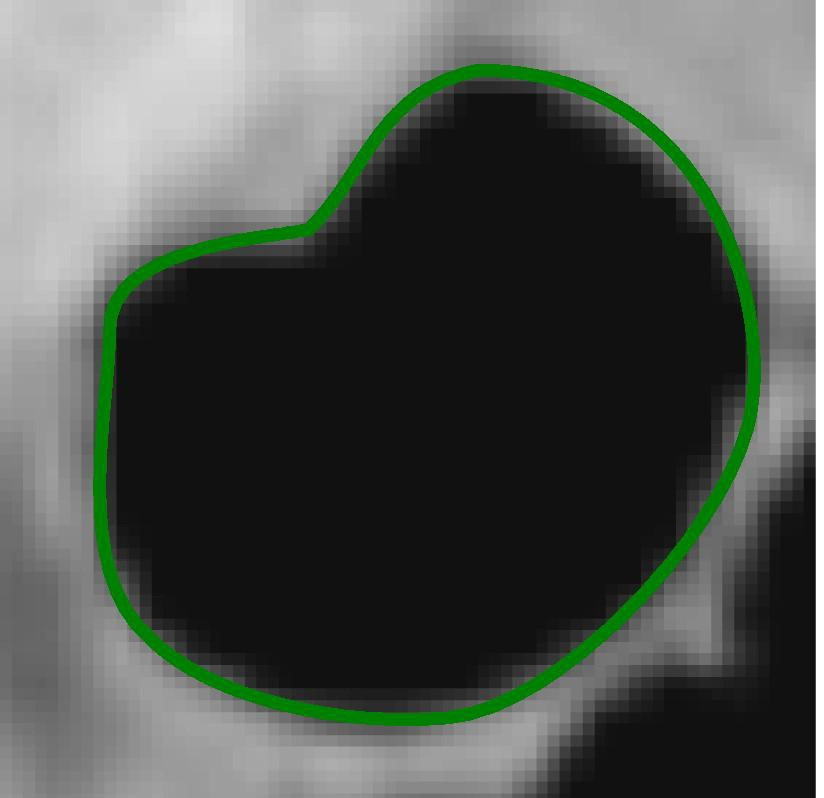
\includegraphics[width=.9\textwidth]{./imagenes/activeContour1-1}
		\subcaption{}\label{activeContour1.1}
	\end{subfigure}
	\begin{subfigure}[t]{2.5in}
		\centering
		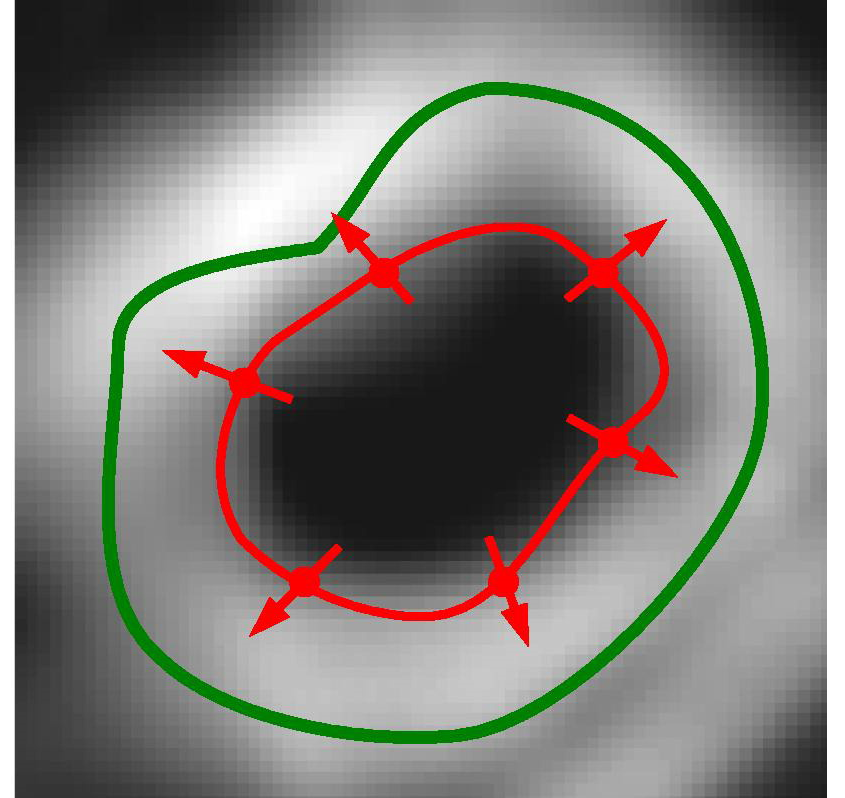
\includegraphics[width=.9\textwidth]{./imagenes/activeContour1-2}
		\subcaption{}\label{activeContour1.2}
	\end{subfigure}
	\caption{Ejemplo de un contorno activo}
	\vspace{2 mm}
	Fuente: \cite{eri2015}
	\label{activeContour1}
\end{figure}

La imagen \ref{activeContour1.1} corresponde a la imagen de entrada, mientras que la imagen \ref{activeContour1.2} corresponde a la convoluci�n de la magnitud gradiente de la imagen de entrada con un filtro pasa bajo gaussiano. La l�nea interior (roja) en la imagen \ref{activeContour1.2} es el contorno activo que se mover� hasta la l�nea exterior (verde) que corresponde con el borde de la imagen original. Un ejemplo de la aplicaci�n de esta t�cnica se puede ver en la figura \ref{activeContour2}.

\begin{figure}[H]
	\captionsetup{justification=centering}	
	\centering
	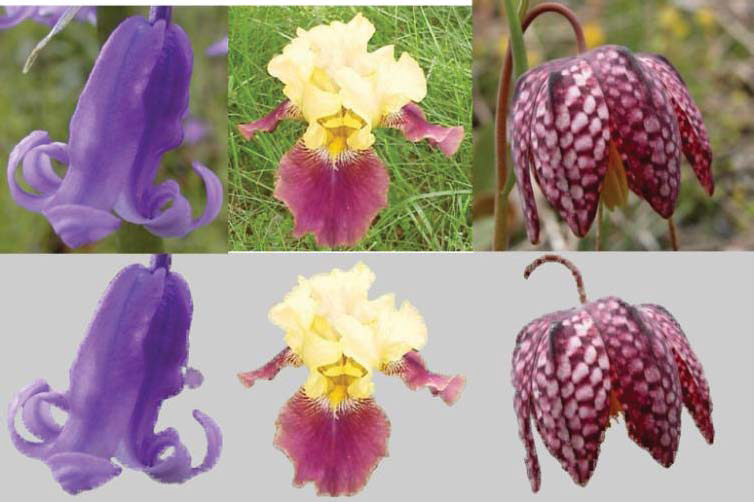
\includegraphics[width=.8\textwidth]{./imagenes/activeContour2}
	\caption{Ejemplo de segmentaci�n de plantas presentando en \cite{suta1} utilizando los contornos activos}
	\vspace{2 mm}
	Fuente: \cite{suta1}	
	\label{activeContour2}
\end{figure}


\subsection{\textit{Level set}}\label{levelSet}
Conjuntos de nivel, o \textit{level set} en ingl�s, es un tipo de segmentaci�n muy parecida a la que hemos explicado en la secci�n \ref{cap:actContour} ya que tambi�n se trata de expandir un contorno dado previamente para encontrar los bordes de la imagen. La ventaja de este m�todo frente al referido es que permite juntar y dividir contornos sin ning�n c�lculo extra necesario.

El contorno est� representado por la funci�n de \textit{level set}, que est� definida en una dimensi�n m�s que las dimensiones de la imagen a segmentar, es decir, para una imagen 2D tendr�amos una superficie de \textit{level set} de tres dimensiones mientras que para una imagen de 3D tendr�amos una superficie de 4D. En el caso de una superficie de 3D �sta tiene una forma c�nica como se puede ver en la figura \ref{levelSet1}. Suponiendo entonces que la imagen a tratar tiene dos dimensiones, podr�amos definir la funci�n de \textit{level set} como $z = \phi(x,y,t)$ que devuelve la altura de la superficie de \textit{level set} en el punto $(x,y)$ del plano de la imagen en el tiempo $t$. El contorno es definido impl�citamente como <<zero \textit{level set}>>, donde la altura del plano respecto a la superficie es cero ($\phi(x,y,t) = 0$). Esto es justo la intersecci�n entre el plano de la imagen y la superficie. V�ase las figuras \ref{levelSet1} y \ref{levelSet2} para ver ilustraciones de la t�cnica de \textit{level set}.

\

Para propagar el contorno se mueve la superficie de \textit{level set} en el eje z, como se puede ver en la figura \ref{levelSet1}. La rapidez y la direcci�n en la que se mueve el contorno est� determinada por como se curva la superficie de \textit{level set}. Suponiendo que cada punto del contorno se mueve en una direcci�n ortogonal frente al contorno con una velocidad F, el contorno evoluciona usando la siguiente PDE (\textit{partial differential equation} o ecuaci�n en derivadas parciales en castellano):

\begin{equation}
\frac{\delta \phi(x,y,t)}{\delta t} = F(x,y,I) |\nabla \phi(x,y,t)|
\end{equation}

Esta funci�n de velocidad var�a dependiendo del punto de la imagen I a tratar y hace que el contorno se expanda a ciertas �reas de la imagen y no lo haga en otras zonas de esta. Normalmente la funci�n de velocidad se define por la intensidad o el gradiente de los p�xeles y por la curva de la funci�n de \textit{level set}.

De la idea de que modificaciones de p�xeles lejanos al contorno no afectan a este surgen varias mejoras de esta t�cnica que tienen en cuenta los p�xeles con los que se trabajar� en cada iteraci�n: \textit{narrow band} y \textit{sparse field methods}. El m�todo de \textit{narrow band} actualiza los p�xeles en una l�nea estrecha alrededor del contorno. El m�todo \textit{sparse field} actualiza los p�xeles vecinos del contorno �nicamente.

\begin{figure}[H]
	\captionsetup{justification=centering}
	\centering
	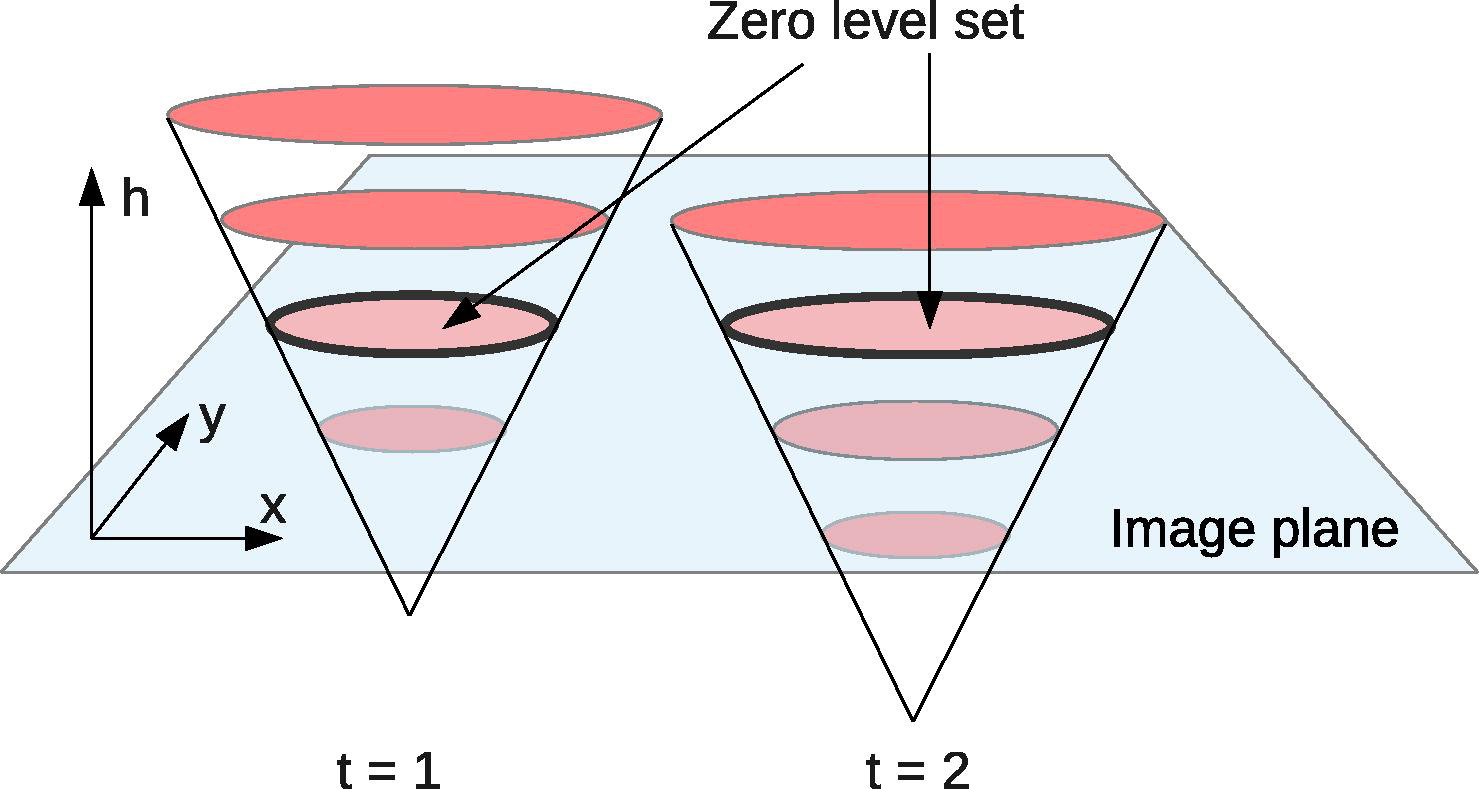
\includegraphics[width=.7\textwidth]{./imagenes/levelSet1}
	\caption{Ilustraci�n de la superficie de \textit{level set}}
	\vspace{2 mm}
	Fuente: \cite{eri2015}
	\label{levelSet1}
\end{figure}
\

\

\

\

\begin{figure}[H]
	\captionsetup{justification=centering}
	\centering
	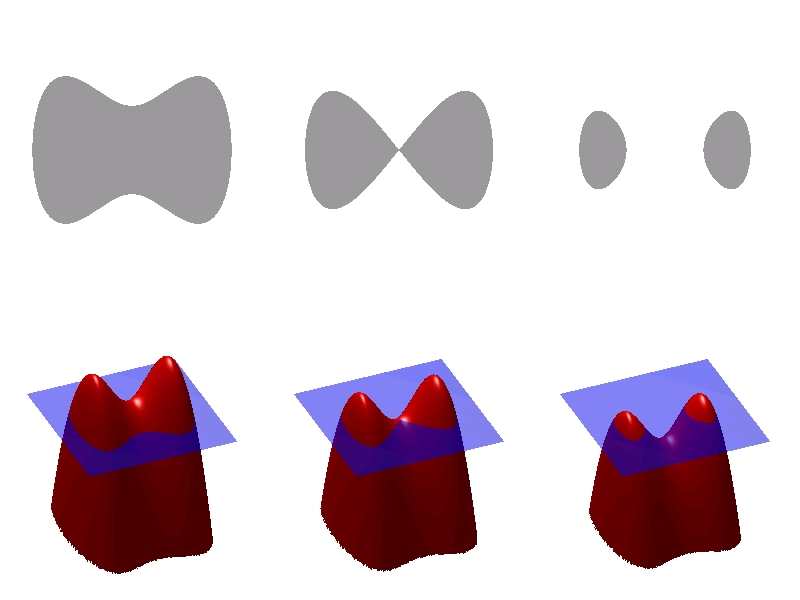
\includegraphics[width=.7\textwidth]{./imagenes/levelSet2}
	\caption{Ilustraci�n del m�todo de \textit{level set}}
	\vspace{2 mm}
	Fuente: commons.wikipedia.org
	\label{levelSet2}
\end{figure}

\section{Segmentaci�n de imagen basada en regiones crecientes}\label{cap:segRegiCreci}

Este tipo de segmentaci�n, m�s conocida como \textit{region growing}, se basa en la idea de que los p�xeles de una regi�n tienen caracter�sticas comunes, como puede ser, la intensidad de gris etc. Por ello, al tener que tratar un nuevo p�xel si este tiene una intensidad de gris parecida a la intensidad de grises que contiene la regi�n significar� que ese punto pertenece a ella. 

Existen varios subgrupos dentro de esta clasificaci�n: t�cnicas basadas en la idea de regiones crecientes, o \textit{region growing} en ingl�s, t�cnicas de \textit{Split/Merge} y t�cnicas basadas en grafos \textit{Graphs cuts}.

\subsection{\textit{Region growing}}

Este subgrupo agrupa todos las t�cnicas que siguen la idea de agrupar los p�xeles con caracter�sticas comunes, como el nivel de gris o el color de �stos. Hay dos t�cnicas conocidas que siguen esta metodolog�a, por lo que en esta ocasi�n explicaremos m�s de una t�cnica de este subgrupo de segmentaci�n.

\subsubsection{$\blacksquare$ \quad \textit{Region growing} o \textit{Seeded-based region growing segmentation}}

Este tipo de segmentaci�n comienza con la selecci�n de un p�xel, denominado a menudo como semilla o \textit{seed} en ingl�s, que est� dentro del objeto de inter�s. Normalmente la semilla se elige manualmente. A partir de ese p�xel semilla (primer punto de la regi�n) se comenzar� a extender la regi�n procesando sus vecinos y a�adi�ndolos en base a un criterio predefinido. Este criterio de inserci�n ser� en base a la intensidad, color o textura de la semilla y los puntos que pertenezcan a la regi�n. Cada vez que se inserta un nuevo punto a la regi�n la caracter�stica que se est� utilizando para realizar la inserci�n se volver� a calcular, por ejemplo, si se utiliza el nivel de gris, se volver� a calcular el valor medio de los niveles de gris que hay en la regi�n generada hasta el momento. De esta manera, la regi�n se ir� expandiendo a�adiendo vecinos hasta que encuentre alguno que no cumpla con la condici�n de inserci�n impuesta por el criterio. Si un punto no ha sido a�adido a ninguna regi�n se podr� a�adir a una regi�n cercana suya si la diferencia entre, por ejemplo, el nivel de gris de este punto y el nivel de gris medio de la regi�n no supera un valor umbral \textit{T} dado. V�ase un ejemplo de esta t�cnica en la figura \ref{regionGrowing1}.

Esta t�cnica es �til cuando la intensidad del fondo y del objeto son muy parecidas pero est�n separadas por un borde <<notable>> o por otra regi�n.
\begin{figure}[H]
	\captionsetup{justification=centering}
	\centering
	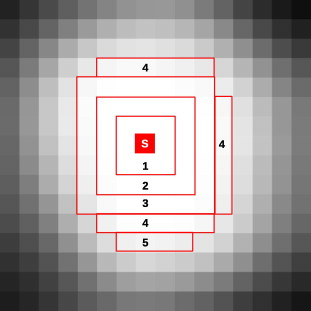
\includegraphics[width=.4\textwidth]{./imagenes/regionGrowing1}
	\caption{Ejemplo del funcionamiento de la t�cnica de \textit{region growing}}
	\vspace{2 mm}
	Fuente: \cite{eri2015}
	\label{regionGrowing1}
\end{figure}
\

\

\

\begin{figure}[H]
	\captionsetup{justification=centering}
	\begin{center}
		\begin{subfigure}[t]{2.5in}
			\centering
			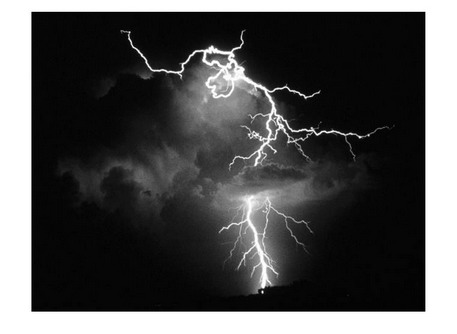
\includegraphics[width=.9\textwidth]{./imagenes/regionGrowing6}
			\subcaption{Imagen original}\label{regionGrowing6}
		\end{subfigure}
	\end{center}	
	\begin{subfigure}[t]{2.5in}
		\centering
		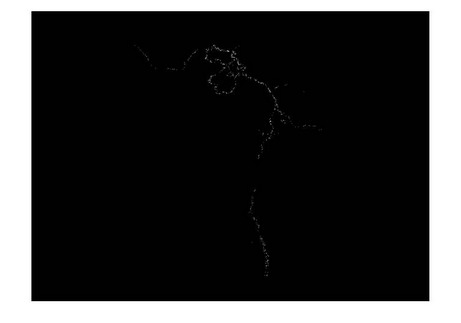
\includegraphics[width=.9\textwidth]{./imagenes/regionGrowing2}
		\subcaption{\textit{Region growing} con un valor umbral T=255}\label{regionGrowing2}
	\end{subfigure}
	\begin{subfigure}[t]{2.5in}
		\centering
		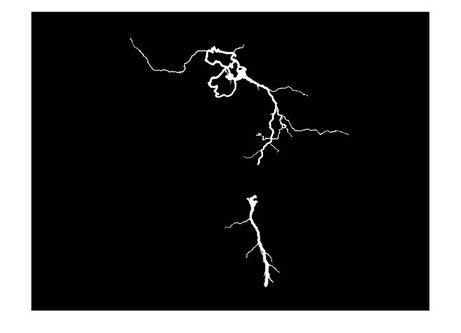
\includegraphics[width=.9\textwidth]{./imagenes/regionGrowing3}
		\subcaption{\textit{Region growing} con un valor umbral T=225}\label{regionGrowing3}
	\end{subfigure}	
	\begin{subfigure}[t]{2.5in}
		\centering
		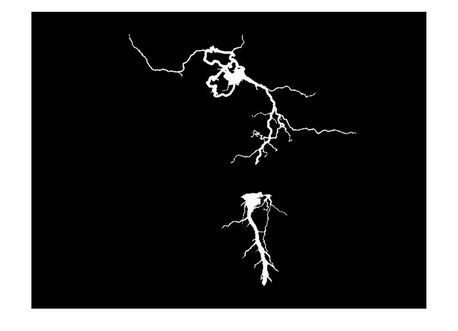
\includegraphics[width=.9\textwidth]{./imagenes/regionGrowing4}
		\subcaption{\textit{Region growing} con un valor umbral T=190}\label{regionGrowing4}
	\end{subfigure}
	\begin{subfigure}[t]{2.5in}
		\centering
		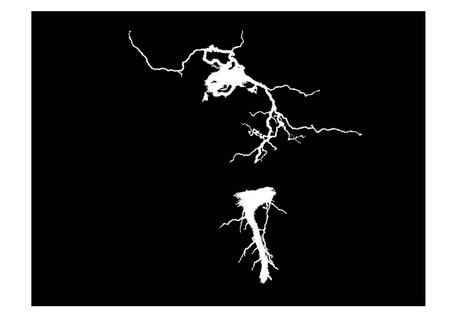
\includegraphics[width=.9\textwidth]{./imagenes/regionGrowing5}
		\subcaption{\textit{Region growing} con un valor umbral T=155}\label{regionGrowing5}
	\end{subfigure}
	\caption{Ejemplo de la t�cnica de \textit{region growing}}
	\centering
	\vspace{2 mm}
	\label{regionGrowingEntera}
	Fuente: commons.wikipedia.org
\end{figure}

En la figura \ref{regionGrowingEntera} se puede ver un ejemplo de la t�cnica de \textit{region growing} donde se quiere encontrar la parte del rayo m�s fuerte en la imagen. Para ello se eligen como semilla los puntos con mayor valor de gris posible(255). El criterio de inserci�n de los p�xeles es tener el "mismo" nivel de gris. En este caso se ha decidido que los puntos que no han sido insertados en una regi�n se inserten en una cercana si superan el valor umbral \textit{T} dado. Por ello en \ref{regionGrowing2} solo aparecen los puntos semilla ya que no se habr�n unido puntos con este criterio y el valor \textit{T} es demasiado alto. En las im�genes \ref{regionGrowing3}, \ref{regionGrowing4} y \ref{regionGrowing5} ese valor \textit{T} se va disminuyendo y cada vez se insertan m�s puntos en la regi�n. 

\

\

\subsubsection{$\blacksquare$ \quad \textit{Watershed}}

La idea principal de esta t�cnica se basa en ver la imagen como una imagen tridimensional donde la tercera dimensi�n es la altura del p�xel. La altura del p�xel est� determinada por su nivel de gris. Topol�gicamente quedar� algo como se puede ver en \ref{watershed1}. En este <<terreno>> creado se podr�n diferenciar hasta tres puntos. Estos puntos son determinados con la analog�a de como una gota de agua caer�a y se mover�a si se precipitase en ese punto. Hay tres tipos de puntos:
\begin{enumerate}
	\item Puntos con un nivel de gris m�nimo local donde la gota se estancar�a.
	\item Puntos en los que la gota caer�a o se deslizar�a hacia un �nico punto m�nimo local.
	\item Puntos en los que la gota podr�a caer hacia m�s de un punto m�nimo local.
\end{enumerate}
El segundo tipo de puntos son nombrados como \textit{watershed} ,o cuencas en castellano, y los del tercer tipo son nombrados como \textit{watersheds lines}, bordes o l�neas de las cuencas en castellano.

El objetivo final de esta t�cnica ser� encontrar los bordes de las cuencas, que representar�n los bordes de la imagen original. Para ello existen varias maneras de hacerlo, la m�s com�n es la t�cnica de \textit{flooding}. La idea es simple, imaginemos que se empieza a echar agua en los puntos de tipo uno, es decir, los que representan un m�nimo local y son <<cuencas>>. El nivel del agua empezar� a subir hasta que llegue a un punto en el que la cuenca se empiece a desbordar y vaya a juntarse con otra cuenca. En ese momento, se construye una presa o un muro de manera que el agua no se desborde. Esas presas o muros construidos ser�n los bordes de las cuencas. Con todas estas presas se habr� conseguido la segmentaci�n de la imagen.

\begin{figure}[H]
	\captionsetup{justification=centering}
	\centering
	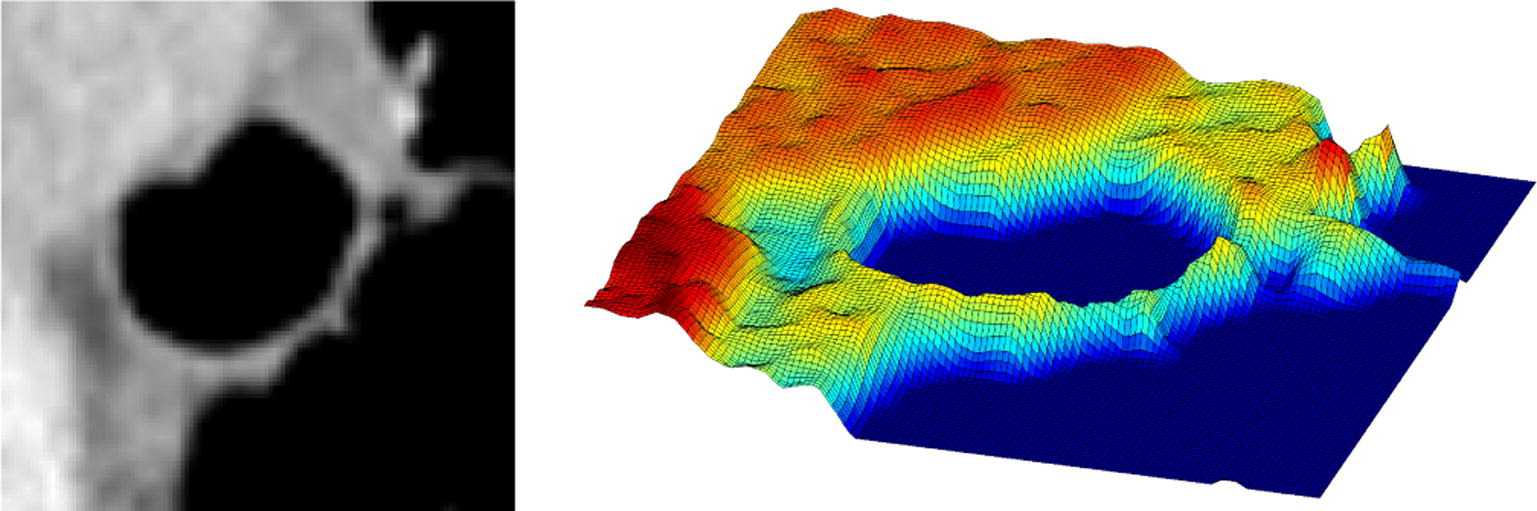
\includegraphics[width=.7\textwidth]{./imagenes/watershed1}
	\caption{Ejemplo del funcionamiento de la t�cnica de \textit{watershed}}
	\vspace{2 mm}
	Fuente: \cite{eri2015}
	\label{watershed1}
\end{figure}
En la figura \ref{watershed2} se puede ver el un ejemplo del funcionamiento de la t�cnica de \textit{watershed} donde la intensidad de los p�xeles de la imagen de la izquierda ser�n la altura de ese mismo punto en la imagen derecha, creando as� ese terreno.

\begin{figure}[H]
	\captionsetup{justification=centering}
	\centering
	
\includegraphics[width=.8\textwidth]{./imagenes/watershed2}
	\caption{Funcionamiento de la t�cnica de \textit{watershed}}
	\vspace{2 mm}	
	Fuente: \textit{http://www.di.ubi.pt/$\sim$agomes/cvm/teoricas/07-regionsegmentation.pdf}	
	\label{watershed2}
\end{figure}

En la figura \ref{watershed3} se muestra el funcionamiento de la t�cnica de \textit{watershed} donde se puede ver como va creciendo el nivel de agua hasta encontrar ese <<punto>> de desbordamiento en el que se marcan los bordes.

\begin{figure}[H]
	\captionsetup{justification=centering}
	\centering
	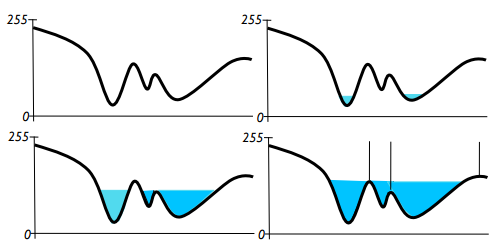
\includegraphics[width=.6\textwidth]{./imagenes/watershed3}
	\caption{Funcionamiento de la t�cnica de \textit{watershed}}
	\vspace{2 mm}		
	Fuente: \textit{http://www.di.ubi.pt/$\sim$agomes/cvm/teoricas/07-regionsegmentation.pdf}
	\label{watershed3}
\end{figure}

\subsection{\textit{Split/Merge}}

La t�cnica de \textit{split}, a diferencia de la t�cnica de \textit{region growing} que empieza con una serie de puntos <<semilla>>, empieza con la imagen entera como una �nica regi�n y va subdividiendo la imagen recursivamente en regiones m�s peque�as en base a un criterio de homogeneidad.

En cuanto a la t�cnica de \textit{merge}, es lo contrario que la de \textit{split}, ya que esta empieza con peque�as regiones de 2x2 o 4x4 y las va juntando entre s� en base a si tienen o no caracter�sticas comunes entre ellas como el nivel de gris, el color, la textura etc.

\subsection{\textit{Graph cut}}

La idea principal de este tipo de segmentaci�n es representar la imagen a tratar como un grafo, donde normalmente cada p�xel es un nodo y tienen aristas con los nodos vecinos. La ventaja de estos algoritmos est� en que pueden llegar a trabajar bien incluso si la separaci�n entre dos regiones est� <<rota>> o es dudosa. Hay varios algoritmos distintos dentro de esta clasificaci�n, en este caso se ha seleccionado el m�todo de segmentaci�n de \textit{Markov}, o \textit{Markov random field (MRF) segmentation} y concretamente una variante de este llamada \textit{graph cut}. 

MRF considera a cada p�xel como un nodo del grafo y tienen aristas con cada p�xel vecino. Sin embargo, cada nodo tiene dos conexiones m�s a un par de nodos especiales llamados \textit{source} (S) y \textit{sink} (T) como se muestra en la figura \ref{graphCuts1}. Se les a�ade un peso a las aristas entre los nodos de manera que los p�xeles que pertenecen al fondo tienen un peso peque�o en la arista que los une con uno de esos dos nodos anteriores y un peso grande con el otro nodo. De forma inversa, los p�xeles que pertenezcan al primer plano tendr�n un peso peque�o con uno de ellos y un peso grande con el otro. Por otro lado, los pesos de las aristas entre los p�xeles son grandes cuando �stos tienen caracter�sticas comunes y un peso peque�o en caso contrario.

La segmentaci�n se realiza aplicando un algoritmo de corte de grafos. El objetivo es minimizar la suma de las aristas por las que se va a cortar el grafo, para ello hay varios algoritmos para buscar el m�nimo corte ha realizar.

\begin{figure}[H]
	\captionsetup{justification=centering}
	\centering
	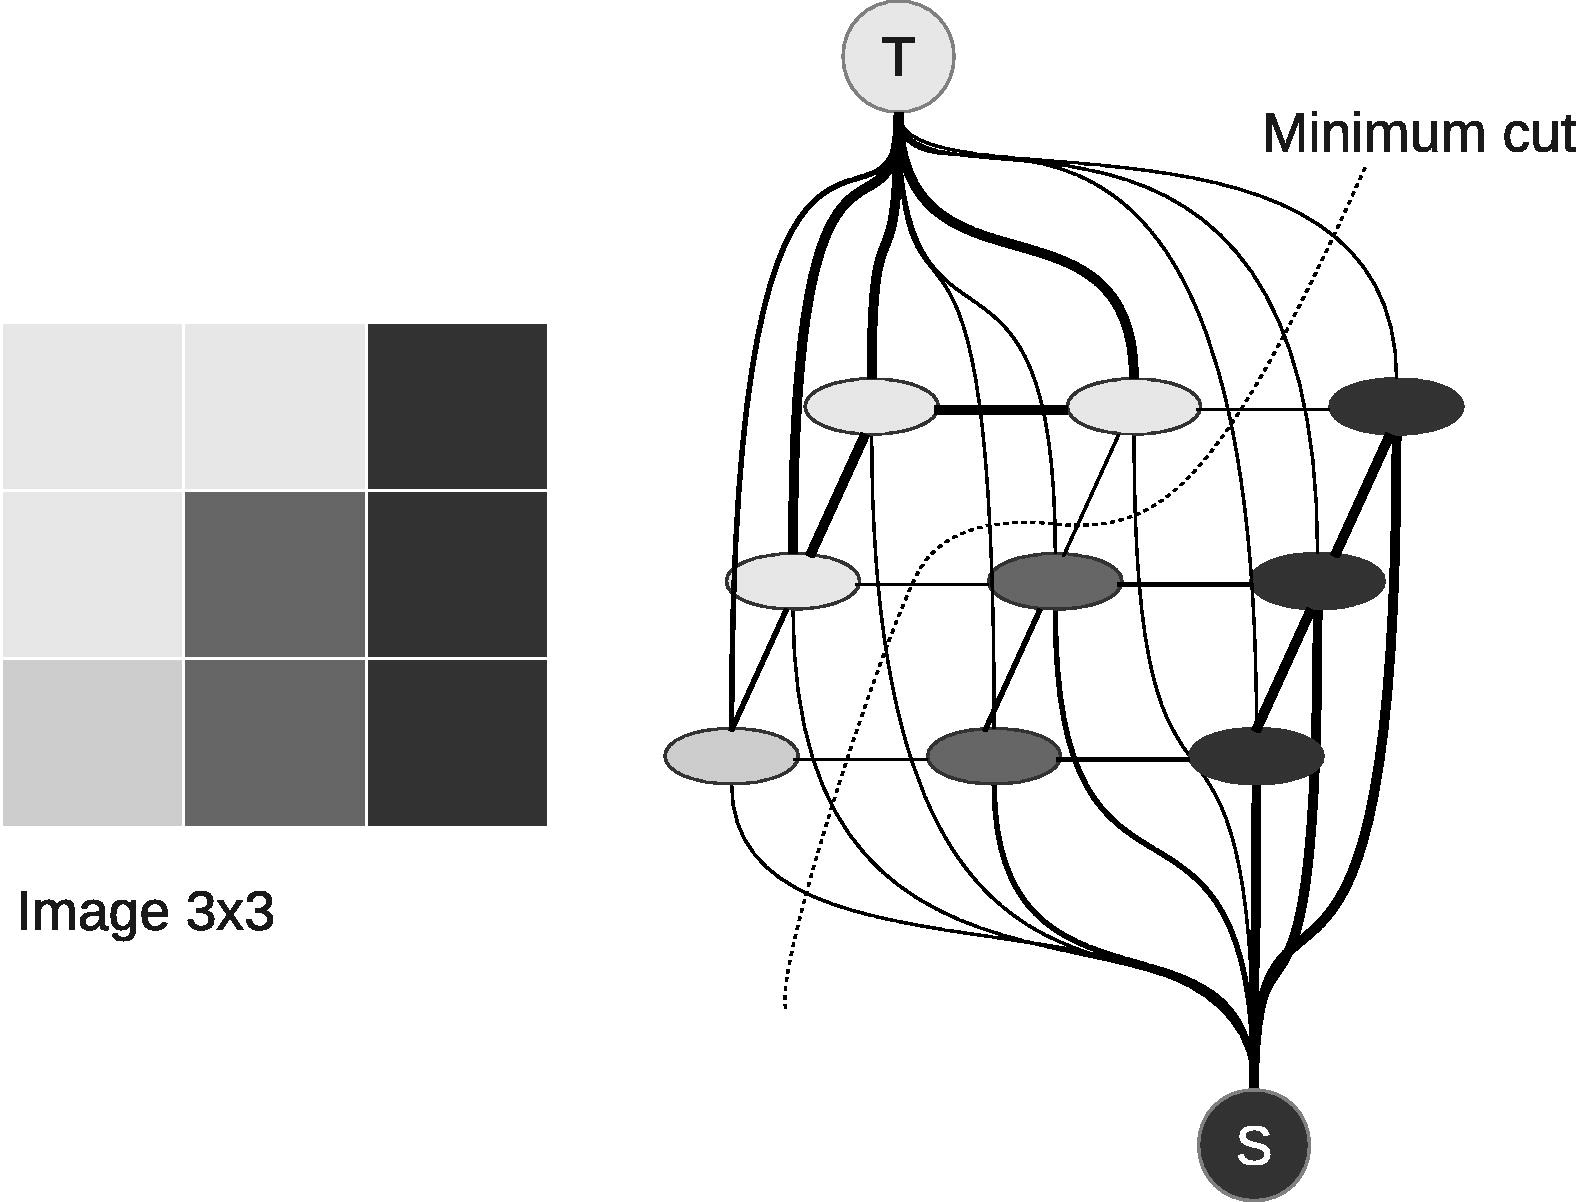
\includegraphics[width=.5\textwidth]{./imagenes/graphCuts1}
	\caption{Funcionamiento de la t�cnica de \textit{graph cut} en una imagen 3x3}
	\vspace{2 mm}		
	Fuente: \cite{eri2015}
	\label{graphCuts1}
\end{figure}

\section{Conclusiones de los tipos de segmentaci�n}\label{sec:conclusiones}

Como se ha podido ver a lo largo de este cap�tulo, hay muchos tipos de t�cnicas de segmentaci�n de im�genes. Adem�s, existen m�s t�cnicas de segmentaci�n que no se han explicado en este trabajo ya que se han a�adido las m�s conocidas y populares con el fin de establecer una base para el lector. 

Aparte de las t�cnicas que no se han explicado hay que decir que existen muchas mejoras, optimizaciones y variantes de todas las t�cnicas de segmentaci�n. Por ello, en este trabajo se han explicado las ideas principales de los algoritmos sin tener en cuenta �sto ya que el trabajo se habr�a extendido demasiado.









\chapter{Optimizaciones y mejoras del algoritmo \textit{level set} original} 


El algoritmo \textit{level set} es uno de los m�s utilizados  como consecuencia del buen rendimiento que obtiene al segmentar im�genes. Existen optimizaciones que lo hacen muy eficiente, como el trabajo que se presentar� a continuaci�n \cite{yong1}, que ser� capaz de satisfacer la demanda que requiere este proyecto.

\

\

\section{Introducci�n}

Como se ha dado a conocer en el apartado \ref{sec:conclusiones} hay muchos tipos de mejoras y optimizaciones de cada t�cnica de segmentaci�n existentes. A la hora de afrontar el problema que el cliente propon�a se ten�a que elegir un tipo de segmentaci�n de las t�cnicas estudiadas. Entre todas ellas se escogi� el algoritmo \textit{level set}, por ser un algoritmo de segmentaci�n eficiente ampliamente utilizado, lo que facilitar�a la b�squeda de informaci�n sobre �l. Adem�s, el cliente recomendaba esta t�cnica, ya que aseguraba que se iban a obtener buenos resultados con ella.

Repasando este algoritmo, las ventajas que tiene son que la segmentaci�n conseguida es precisa y que no a�ade sobrecoste al hacer la divisi�n o uni�n del contorno. Sin embargo, el algoritmo se basa en la resoluci�n de ecuaciones diferenciales, lo que supone que el algoritmo sea costoso y lento. Se han desarrollado varias implementaciones en GPU \cite{eri2015}, tambi�n sobre im�genes 3D \cite{aaron1}, y en proyectos de fin de carrera tambi�n se utilizan GPUs \cite{cudaseg} etc. De la misma manera, tambi�n se han desarrollado paralelizaciones del algoritmo para arquitecturas SMP(\textit{Symmetric Multi-Processing}) \cite{jeon1} o para arquitecturas de memoria distribuida con MPI(\textit{Message Passing Interface})  \cite{moha1}. 

Hay muchos art�culos sobre este algoritmo, alguna implementaci�n paralela realizada sobre el algoritmo original y, por lo tanto, a pesar de la paralelizaci�n, los tiempos que obtienen siguen siendo elevados para las restricciones de este proyecto. Estas paralelizaciones y otras t�cnicas de optimizaci�n se centran siempre en resolver las PDEs asociadas a la evoluci�n del \textit{level set}. Sin embargo, para muchos problemas de imagen, como la segmentaci�n, no es necesario tanta precisi�n, ya que el objetivo final es encontrar los bordes de los objetos. En este caso, la evoluci�n del proceso no tiene tanto inter�s como el resultado final. Siguiendo esta idea Shi y Karl presentaron un art�culo muy interesante que ser� la base de la segmentaci�n realizada en este proyecto \cite{yong1}.

\

\

\section{Aproximaci�n a la t�cnica de \textit{level set}}

Como se ha mencionado anteriormente para el objetivo de este proyecto, no se tienen por qu� resolver las PDEs en el algoritmo \textit{level set} ya que, para una segmentaci�n, importa m�s el resultado final que la evoluci�n propia del algoritmo. Adem�s, la resoluci�n de las PDEs conlleva que se tengan que realizar reinicializaciones de la funci�n de \textit{level set} (representada con la letra $\phi$) lo que implica a�n m�s c�lculo. El trabajo presentado por Shi y Karl \cite{yong1} elimina la reinicializaci�n al tener una colecci�n de enteros (los cuales representan la funci�n $\phi$) que cambian din�micamente seg�n va propag�ndose el contorno y, adem�s, no calculan las PDEs. Estas dos mejoras elementales hace que su algoritmo sea mucho m�s r�pido que el \textit{level set} original. 

En este trabajo se presenta una nueva estrategia de implementaci�n del m�todo de \textit{level set}. Para el caso de un espacio eucl�deo de dos dimensiones, una curva C es representada impl�citamente como el \textit{zero level set} de una funci�n $\phi$ definida en una cuadr�cula como se muestra en la figura \ref{aproxLevelSet}. La funci�n $\phi$ tendr� un valor negativo dentro de la curva C y un valor positivo fuera de ella, por eso se dice que representa impl�citamente a la curva C. 

Se definen dos listas de vecindad en esta cuadr�cula, $L_{in}$ y $L_{out}$. En la imagen se puede ver que el movimiento de la curva C se puede conseguir moviendo un punto de una lista a otra.

Se asume que la funci�n $\phi$ est� definida sobre un dominio $D \subset R^k$ y est� discretizada sobre una rejilla de tama�o $M_1 \times M_2 \times ... \times M_k$. Estando entonces en una representaci�n de dos dimensiones, y siguiendo el ejemplo de la rejilla mostrada anteriormente se pueden definir dos listas de vecindad del contorno C: $L_{in}$ y $L_{out}$.

\

$L_{in} = \{x \ | \ \phi(x) < 0$ y $  \exists y \in N(x)$ tal que $\phi(y) > 0\}$

\

$L_{out} = \{x \ | \ \phi(x) > 0$ y $  \exists y \in N(x)$ tal que $\phi(y) < 0\}$

\

\begin{figure}[H]
	\captionsetup{justification=centering}	
	\begin{center}
		\begin{subfigure}[t]{2.5in}
			\centering
			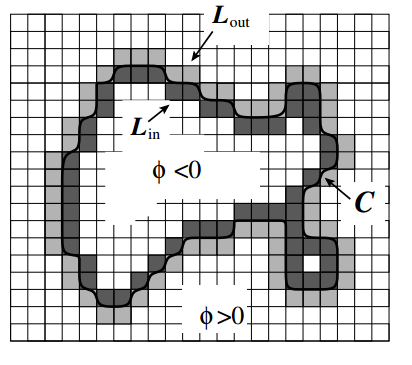
\includegraphics[width=1\textwidth]{./imagenes/aproxLevelSet1}
			\subcaption{}\label{aproxLevelSet1}
		\end{subfigure}
		\begin{subfigure}[t]{2.5in}
			\centering
			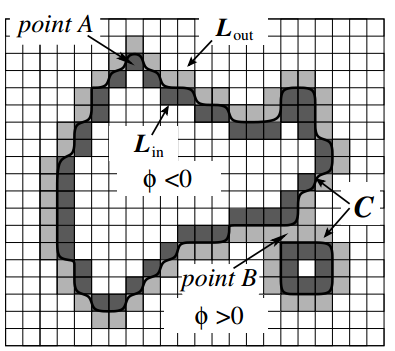
\includegraphics[width=1\textwidth]{./imagenes/aproxLevelSet2}	
			\subcaption{}\label{aproxLevelSet2}
		\end{subfigure}
	\end{center}
	\caption{Representaci�n de la curva C}
	\vspace{2 mm}		
	\centering
	Fuente: \cite{yong1}	
	\label{aproxLevelSet}
\end{figure}	

Siendo x una coordenada de la rejilla denotada como $x = {x_1,x_2,...,x_k}$ y $N(x)$ como un vecino de x con valor discreto definido como:
\begin{equation}
N(x) = \{y \in D \ | \ \sum_{k=1}^{K} |y_k - x_k| = 1\}  \ \forall x \in D
\end{equation}

Como podemos observar en la figura \ref{aproxLevelSet} la lista $L_{in}$ est� formada por los puntos de la rejilla que est�n dentro de la curva C y $L_{out}$ est� formada por los puntos de la rejilla que est�n fuera de C. Por lo tanto, como se puede ver en las definiciones formales de las listas, cada punto de ellas tiene que tener un punto vecino de la otra lista, de manera que las dos est�n "pegadas".

Recordando lo visto en la secci�n de explicaci�n del \textit{level set}(\ref{levelSet}) en el cl�sico \textit{level set} la siguiente PDE es resuelta para evolucionar el contorno C bajo una funci�n de velocidad F:
\begin{equation}\label{speedLevelSet}
\frac{d\phi}{dt} + F|\nabla \phi| = 0
\end{equation}
La figura \ref{aproxLevelSet2} muestra el proceso evolutivo de la curva C de la figura \ref{aproxLevelSet1}. En el punto marcado como A la curva se ha movido hacia fuera lo que ha modificado el valor de la funci�n $\phi$ de positivo a negativo. En el punto B la curva se ha movido hacia dentro, partiendo la curva en dos y cambiando el valor de la funci�n $\phi$ de negativo a positivo. Todo esto tambi�n ocurre en el \textit{level set} original, con la diferencia de que la resoluci�n de la PDE mostrada en la ecuaci�n \ref{speedLevelSet} tiene un coste elevado. Se consiguen los mismos resultados finales f�cilmente si se usa la relaci�n entre C, $L_{in}$ y $L_{out}$. Para mover la curva hacia fuera en el punto A de la rejilla tendremos que pasar el punto de la lista $L_{out}$ a $L_{in}$. De manera similar, para mover la curva hacia dentro en el punto B tendremos que cambiar el punto B de $L_{in}$ a $L_{out}$. En general, con aplicar dichas operaciones se va moviendo la curva hacia cualquier punto con el m�nimo coste operacional. 


\subsubsection{Algoritmo}

Para la realizaci�n del algoritmo son necesarias estas estructuras:

\begin{itemize}
	\item Un array para la funci�n de \textit{level set }$\phi$;
	\item Un array para la velocidad (F) con la que se propagar� la curva;
	\item Dos listas de vecindad de la curva: $L_{in}$ y $L_{out}$.	
\end{itemize}

Nombraremos a los puntos que est�n dentro de C pero no en la lista $L_{in}$ como <<puntos interiores>> y a los que est�n fuera de C pero que no pertenecen a $L_{out}$ como <<puntos exteriores>>. Para agilizar a�n m�s el c�lculo, los valores que puede tomar la funci�n $\phi$ son cuatro enteros: {-3, -1, 1, 3}.
\begin{equation}
\phi (x) = 
\left \{
\begin{array}{rcl}
3 & si & x \mbox{ es un punto exterior} \\
1 & si & x \in L_{out} \\ 
-1 & si & x \in L_{in} \\
-3 & si & x \mbox{ es un punto interior}
\end{array}
\right .
\end{equation}

 Para la funci�n F de velocidad s�lo se usa el signo, por lo que tambi�n es un \textit{array} de enteros con los valores: {1, 0, -1}. En cuanto a las listas, son listas ligadas de manera que la inserci�n y el borrado de puntos se pueden hacer de manera r�pida. 
 
 Antes de presentar el algoritmo se aclarar�n ciertas cuestiones. Para empezar, hay dos operaciones b�sicas que se utilizan en el algoritmo:
 
 \begin{itemize}
 	\item  La operaci�n \textit{switch\_in()} para un punto x $\in L_{out}$ se define como:
 	switch\_in(x):
 	\begin{itemize}
 		\item Paso 1: Se quita el punto de $L_{out}$ y se pasa a $L_{in}$. Se cambia el valor de $\phi$ en ese punto: $\phi$(x) = -1.
 		\item Paso 2: Se a�aden los puntos vecinos de x a $L_{out}$ y se cambian sus respectivos valores en $\phi$. M�s formalmente: $\forall y$ $\in$ N(x) que satisfaga $\phi(y) = 3$ se a�ade $y$ a $L_{out}$ y se pone $\phi(y) = 1$
 	\end{itemize}
 	Con esta operaci�n se mueve el contorno un punto de la rejilla hacia fuera. 
 	\item Similarmente se define la operaci�n \textit{switch\_out()} para un punto x $\in$ $L_{in}$:
 	 switch\_out(x): 	 
 	 \begin{itemize}
 	 	\item Paso 1: Se quita el punto de  $L_{in}$ y se pasa a $L_{out}$. Se cambia el valor de $\phi$ en ese punto: $\phi$(x) = 1.
 	 	\item Paso 2: Se a�aden los puntos vecinos de x a $L_{in}$ y se cambia sus respectivos valores en $\phi$. M�s formalmente: $\forall y $ $\in$ N(x) que satisfaga $\phi(y) = -3$ se a�ade $y$ a $L_{out}$ y se pone $\phi(y) = -1$
 	 \end{itemize}
 	Con esta operaci�n se mueve el contorno un punto de la rejilla hacia dentro. 
 \end{itemize}

Por otro lado, la funci�n F de velocidad presentada antes, normalmente se suele separar en dos velocidades: $F_{ext}$ que depende de los datos y $F_{int}$ para la realizaci�n de un suavizado del contorno. La velocidad $F_{int}$ es normalmente la curvatura de la curva \cite{chan}. Sin embargo, esta evaluaci�n de la curva usando la funci�n $\phi$ suele ser computacionalmente costosa. Tras varios pasos esta funci�n de velocidad $F_{int}$ puede llegar a ser determinada por un filtro Gaussiano que puede ser aproximado con operaciones con enteros, por lo que se reduce el c�mputo. Adem�s, al separar las dos velocidades, no tiene por qu� hacerse el suavizado despu�s de cada iteraci�n de evoluci�n del contorno como en otros trabajos \cite{yong1}, sino que se realizar� cuando se satisfaga cierta condici�n, lo que reduce a�n m�s el coste. Con esto entonces, el algoritmo tendr� dos ciclos principales: el primer ciclo en el que se expandir� o evolucionar� el contorno y el segundo ciclo (que se realizar� de vez en cuando) en el que se suavizar� el contorno para que se siga expandiendo con normalidad. 


\begin{table}[H]
	\small
	\centering
	\begin{tabular}{|l|}
		\hline		
		\tabitem Paso 1: Inicializar el <<array>> $\phi$, $F_{ext}$ y las dos listas $L_{out}$ y $L_{in}$. \\
		\tabitem Paso 2: Primer ciclo donde se escanean las dos listas para actualizar $\phi$, $L_{out}$ y $L_{in}$. \\
		\quad \quad \quad \quad - Se calcula la velocidad para cada punto de $L_{out}$ y $L_{in}$. \\
		\quad \quad \quad \quad - Evoluci�n hacia fuera. Recorremos la lista $L_{out}$ y se hace  la operaci�n \\ 
		\quad \quad \quad \quad \ \ \textit{switch\_in(x)} $\forall x \in L_{out}$ si $F_{ext}$(x) $>$ 0. \\ 
		\quad \quad \quad \quad - Se eliminan los puntos redundantes en $L_{in}$ (v�ase la figura \ref{switchLevelSet}).\\ 
		\quad \quad \quad \quad \ \ Para ello se tendr� que recorrer la lista y para cada punto $x \in L_{in}$,\\
		\quad \quad \quad \quad \ \ si $\forall y \in N(x); \phi(y) < 0$, se borra $x$ de $L_{in}$ y se cambia $\phi(x) = -3$. \\ 
		\quad \quad \quad \quad - Evoluci�n hacia dentro. Recorremos la lista $L_{in}$ y se hace  la operaci�n \\ 
		\quad \quad \quad \quad \ \ \textit{switch\_out(x)} $\forall x \in L_{in}$ si F(x) $<$ 0. \\ 
		\quad \quad \quad \quad - Se eliminan los puntos redundantes en $L_{out}$. Para ello se tendr� que \\
		\quad \quad \quad \quad \ \ recorrer la lista y para cada punto $x \in L_{out}$,\\
		\quad \quad \quad \quad \ \ si $\forall y \in N(x); \phi(y) > 0$, se borra $x$ de $L_{out}$ y se cambia $\phi(x) = 3$. \\
		\quad \quad \quad \quad - Se comprueba la condici�n de parada y si se satisface se continua al paso 3, \\ 
		\quad \quad \quad \quad \ \ si no, seguiremos en el paso 2. \\
		\tabitem Paso 3: Segundo ciclo donde se realiza un suavizado del contorno con un \\ 
		\quad \quad \quad \quad \ \ filtro Gaussiano. \\
		\quad \quad \quad \quad - Evoluci�n hacia fuera. Recorremos la lista $L_{out}$ y se calcula G $\oplus \ \phi(X)$. \\ 
		\quad \quad \quad \quad \ \ Si  G $\oplus \phi(X) <$ 0 se realiza la operaci�n \textit{switch\_in(x)} \\ 
		\quad \quad \quad \quad - Se eliminan los puntos redundantes en $L_{in}$ (v�ase la figura \ref{switchLevelSet}).\\ 
		\quad \quad \quad \quad \ \ Para ello se tendr� que recorrer la lista y para cada punto $x \in L_{in}$,\\
		\quad \quad \quad \quad \ \ si $\forall y \in N(x); \phi(y) < 0$, se borra $x$ de $L_{in}$ y se cambia $\phi(x) = -3$. \\ 
		\quad \quad \quad \quad - Evoluci�n hacia dentro. Recorremos la lista $L_{in}$ y se calcula  G $\oplus \ \phi(X)$. \\ 
		\quad \quad \quad \quad \ \ Si G $\oplus \phi(X)$ > 0 se realiza la operaci�n \textit{switch\_out(x)}  \\ 
		\quad \quad \quad \quad - Se eliminan los puntos redundantes en $L_{out}$. Para ello se tendr� que \\
		\quad \quad \quad \quad \ \ recorrer la lista y para cada punto $x \in L_{out}$,\\
		\quad \quad \quad \quad \ \ si $\forall y \in N(x); \phi(y) > 0$, se borra $x$ de $L_{out}$ y se cambia $\phi(x) = 3$. \\
		\tabitem Paso 4:  Si se satisface la condici�n de parada del ciclo uno, se termina el algoritmo, \\
		\quad \quad \quad \quad \ \ si no, se vuelve al paso 2. \\
		\hline
	\end{tabular}
	\caption{Algoritmo completo de la aproximaci�n del \textit{level set}}
	\vspace{2 mm}		
	Fuente: \cite{yong1}
	\label{algoritmoFastLevelSet}
\end{table}


Aclaradas las cuestiones anteriores, el (r�pido) algoritmo \textit{level set} \cite{yong1} se muestra en la tabla \ref{algoritmoFastLevelSet}. Como se puede observar el segundo ciclo es pr�cticamente igual al primer ciclo, a excepci�n de que la condici�n de cambiar un punto de una lista a otra, es decir, de hacer una de las operaciones \textit{switch()} que se han explicado anteriormente, depende de un filtro Gaussiano (G) en el segundo ciclo (velocidad $F_{int}$) y de los datos en el primer ciclo (velocidad $F_{ext}$). Las operaciones de \textit{switch\_in()} se realizar�n cuando el valor de $F$ ($F_{ext}$ en el primer ciclo y $F_{int}$ en el segundo ciclo) sea positivo, que querr� decir que el contorno deber� expandirse hacia fuera y las operaciones de \textit{switch\_out()} se realizar�n cuando el valor de $F$ ($F_{ext}$ en el primer ciclo y $F_{int}$ en el segundo ciclo) sea negativo, contrayendo el contorno en ese punto. V�ase la figura \ref{switchLevelSet} como ejemplo de expansi�n del contorno en un p�xel.

Repasando un poco m�s el algoritmo \ref{algoritmoFastLevelSet} queda por aclarar las condiciones de parada del algoritmo. As� pues, el algoritmo se parar� en el caso de que se cumpla una de estas dos condiciones:

\begin{enumerate}
	\item Que la velocidad $F_{ext}$ de toda la vecindad del contorno cumpla con:
	\begin{enumerate}	
		\item $F(x) \leq 0 \ \forall x \in L_{out}$, es decir, que no se tenga que expandir el contorno por ninguno de sus puntos.
		\item $F(x) \geq 0 \ \forall x \in L_{in}$, es decir, que no se tenga que contraer el contorno en ninguno de sus puntos.
	\end{enumerate}
	\item Que se alcance un determinado n�mero de iteraciones establecido.
\end{enumerate}
 
Para finalizar, el coste del algoritmo es de orden O(2A($P_1$ + $P_2$)), donde A es el n�mero de puntos entre el primer contorno creado y el �ltimo ya evolucionado, $P_1$ y $P_2$ el coste de las operaciones de switch() y el coste que tiene el borrado y la inserci�n de los puntos en las listas respectivamente. El escalar 2 es debido a que los puntos pueden llegar a pertenecer a una lista primero, y luego a otra, realizando as� las operaciones dos veces. N�tese que ese A ser� mucho menor que la $m \times n$ que ser�a la anchura (m) por la altura (n) de la imagen, ya que si en la imagen se detectan varios objetos, el tama�o en puntos o p�xeles de cada objeto se restar� a ese $m \times n$.
   
 \begin{figure}[]
 	\captionsetup{justification=centering}
 	\centering
 	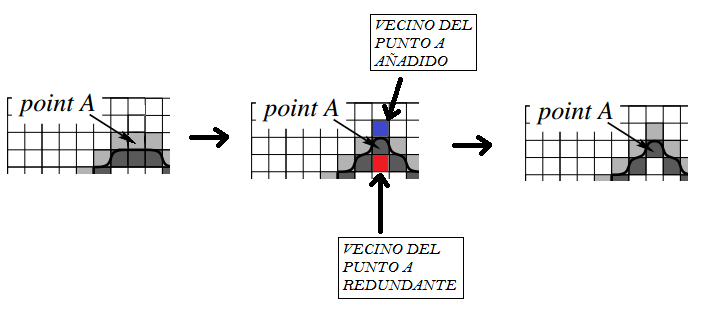
\includegraphics[width=.8\textwidth]{./imagenes/switchLevelSet}
 	\caption{Ejemplo de expansi�n del contorno un p�xel hac�a fuera. Operaciones que se realizan continuamente en el paso 2 y 3 del algoritmo}
	\vspace{2 mm}		
 	Fuente: modificaciones de im�genes en \cite{yong1}	
 	\label{switchLevelSet}
 \end{figure}
 
 
 
\section{Evoluci�n del contorno}

Se ha querido a�adir esta secci�n para destacar y hablar un poco m�s en detalle sobre la evoluci�n de la curva que se ha elegido en esta aproximaci�n: la presentada en \cite{chan}. Este popular trabajo es conocido como \textit{Chan-Vese model} y a diferencia de como se realizaba la segmentaci�n, utilizando el uso de detectores de bordes basados en el gradiente, este trabajo realiza la detecci�n de objetos cuyos bordes no tienen porque estar definidos por el gradiente. Este m�todo es flexible y potente, capaz de realizar la segmentaci�n de muchos tipos de im�genes que con m�todos tradicionales como \textit{thresholding} o m�todos basados en el gradiente no pod�an realizarse. Este m�todo tambi�n permite que el contorno se inicialice dentro del objeto o incluso entre el objeto y el fondo ya que el resultado final ser� siempre el mismo. La figura \ref{chanVese} muestra las posibles inicializaciones. Esta caracter�stica ser� de utilidad como se comentar� en posteriores cap�tulos.

Para tener una m�nima idea del avance que esto supuso en la segmentaci�n de im�genes, si volvemos a utilizar el buscador \cite{ieee1} y encontramos dicho art�culo, el n�mero de citaciones de otros art�culos registrados en ese explorador alcanza casi la cifra de 2.000, lo que tampoco quiere decir que no haya m�s trabajos no registrados en \cite{ieee1} que lo citen. 
 
\begin{figure}[H]
	\captionsetup{justification=centering}	
	\begin{center}
		\begin{subfigure}[t]{2.5in}
			\centering
			
\includegraphics[width=.5\textwidth]{./imagenes/chanVese1}
			\subcaption{}\label{chanVese1}
		\end{subfigure}
		\begin{subfigure}[t]{2.5in}
			\centering
			
\includegraphics[width=.5\textwidth]{./imagenes/chanVese2}	
			\subcaption{}\label{chanVese2}
		\end{subfigure}
		\begin{subfigure}[t]{2.5in}
			\centering
			
\includegraphics[width=.5\textwidth]{./imagenes/chanVese3}	
			\subcaption{}\label{chanVese3}
		\end{subfigure}
		\begin{subfigure}[t]{2.5in}
			\centering
			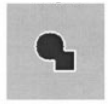
\includegraphics[width=.5\textwidth]{./imagenes/chanVese4}	
			\subcaption{}\label{chanVese4}
		\end{subfigure}
	\end{center}
	\caption{Posibles inicializaciones del contorno con el m�todo de Chan-Vese}
	\vspace{2 mm}	
	\centering	
 	Fuente: \cite{chan}	
	\label{chanVese}
\end{figure} 
 
 
 
 
 
 
\chapter{Implementaci�n de la aproximaci�n y Ofeli}

Una vez encontrada una t�cnica que contemplara los requisitos del proyecto, se empez� a buscar alguna implementaci�n sobre esta t�cnica. En esa b�squeda se encontr� un trabajo llamado Ofeli (\textit{Open, Fast and Efficient Level set Implementation}) \cite{ofeli}. Este trabajo est� desarrollado con Qt que es una de librer�as multiplataforma para la realizaci�n de aplicaciones con GUI (\textit{graphical user interface}) en C++. Esta aplicaci�n es muy completa ya que, aparte del algoritmo de inter�s, implementa varias funcionalidades extra como varios tipos de filtrado, preprocesamiento, varios tipos de evoluci�n del contorno, etc.

\section{Ofeli}

En esta secci�n se explicar� la estructura de la implementaci�n y las clases que se utilizan en este trabajo. Se realizar� un esquema general para que el lector pueda comprender cu�les son los procesos o pautas que se dan en esta implementaci�n para poder segmentar una imagen.


\subsection{Estructura}

La implementaci�n est� formada por varias clases que se han dividido en dos tipos: las clases o ficheros que pertenecen a la GUI (etiquetadas con la palabra <<GUI->> por delante de sus nombres) y las clases que pertenecen a la implementaci�n del algoritmo (etiquetadas con la palabra <<Impl->>).

\begin{enumerate}
	\item Impl-\textbf{ActiveContour}: clase padre de todos los tipos de contornos. Formada por lo ficheros:
		\begin{enumerate}
			\item activecontour.cpp
			\item activecontour.hpp
		\end{enumerate}
	\item Impl-\textbf{ACwithoutEdges}: clase que implementa el contorno que evolucionar� en una imagen a escala de grises. Formada por lo ficheros:
	\begin{enumerate}
		\item ac\_withoutedges.cpp
		\item ac\_withoutedges.hpp
	\end{enumerate}
	\item Impl-ACwithoutEdgesYUV: clase que implementa el contorno que evolucionar� en una imagen a color. Formada por lo ficheros:
	\begin{enumerate}
		\item ac\_withoutedges\_yuv.cpp
		\item ac\_withoutedges\_yuv.hpp
	\end{enumerate}
	\item Impl-\textbf{list}: implementaci�n de una lista ligada gen�rica. Formada por lo ficheros:
	\begin{enumerate}
		\item linked\_list.tpp
		\item linked\_list.hpp
	\end{enumerate}
	\item Impl-Filters: clase que implementa los filtros que se le pueden aplicar a la imagen antes de realizar la segmentaci�n. Formada por lo ficheros:
	\begin{enumerate}
		\item filters.cpp
		\item filters.hpp
	\end{enumerate}
	\item Impl-GeodesicAC: clase que implementa un contorno geod�sico. Formada por lo ficheros:
	\begin{enumerate}
		\item geodesic\_ac.cpp
		\item geodesic\_ac.hpp
	\end{enumerate}
	\item Impl-HausdorffDistance: clase que implementa la distancia de Hausdorff. Formada por lo ficheros:
	\begin{enumerate}
		\item hausdorff\_distance.cpp
		\item hausdorff\_distance.hpp
	\end{enumerate}
	\item GUI-ImageViewer: formada por los ficheros:
	\begin{enumerate}
		\item imageviewer.cpp
		\item imageviewer.hpp
	\end{enumerate}
	\item GUI-PixmapWidget: formada por los ficheros:
	\begin{enumerate}
		\item pixmapwidget.cpp
		\item pixmapwidget.hpp
	\end{enumerate}
\end{enumerate}
 
Se han resaltado las tres clases que interesar�n: \textit{ActiveContour}, \textit{ACwithoutEdges} y \textit{list}. Las dem�s clases a�aden funcionalidades extra que no son necesarias en este proyecto.
 
\subsection{Esquema general}

 \begin{figure}[H]
 	\captionsetup{justification=centering}
 	\centering
 	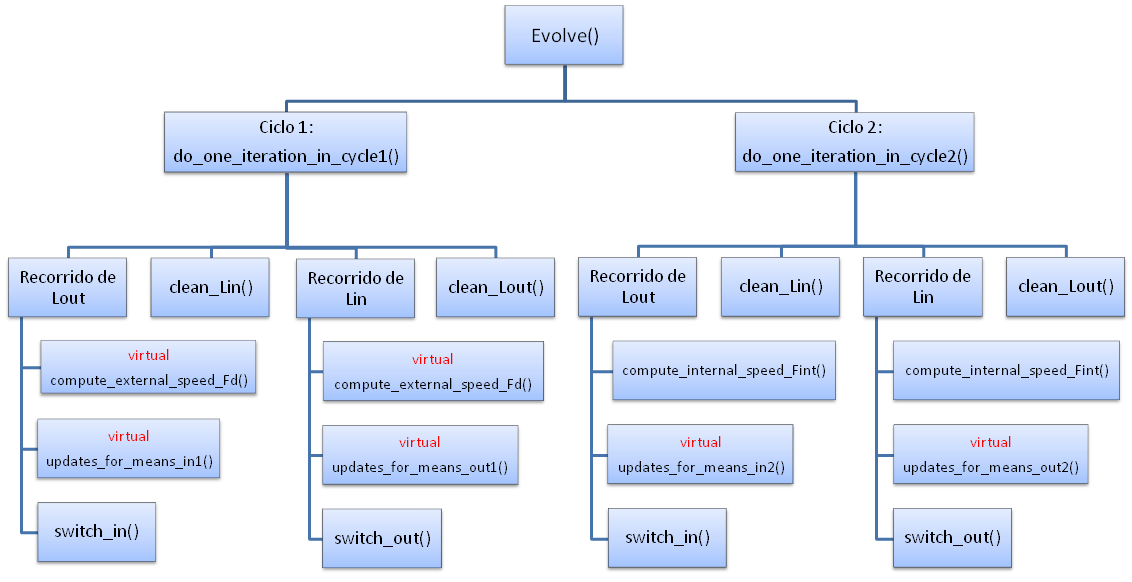
\includegraphics[width=1.3\textwidth]{./imagenes/esquemaOfeli}
 	\caption{Esquema de las funciones utilizadas en el trabajo de Ofeli para realizar el algoritmo \textit{level set }aproximado}	
 	\label{esquemaOfeli}
 \end{figure}

Como se puede observar la estructura del c�digo es pr�cticamente igual al algoritmo de aproximaci�n presentado en \ref{algoritmoFastLevelSet} exceptuando que en esta implementaci�n la velocidad de cada punto se calcula a la hora de tratar �ste, no se calculan todas las velocidades de todos los puntos a la vez como se sugiere en el algoritmo \ref{algoritmoFastLevelSet}. El c�lculo de estas velocidades son las funciones  \textit{compute\_(internal/external)\_speed\_($Fd/F_{int}$)} que se pueden ver en el esquema \ref{esquemaOfeli}. Las funciones  \textit{update\_for\_means\_(in/out)(1/2)} que no est�n en el algoritmo de aproximaci�n presentado en \ref{algoritmoFastLevelSet} se realizan para poder <<adaptar>> el contorno a la imagen de manera que �ste pueda evolucionar independientemente de los niveles de gris que se est�n utilizando en la imagen. Esto se refiere a que se va haciendo una media de las intensidades de los puntos pertenecientes a las listas que representan impl�citamente el contorno, es decir, $L_{out}$ y $L_{in}$, de manera que el umbral con el que se va decidiendo la velocidad de cada punto va cambiando en funci�n de los puntos que representan el contorno.

Las funciones definidas como \textit{clean()} son las limpiezas de las listas sobre puntos redundantes que pudiera haber que se nombra en el algoritmo \ref{algoritmoFastLevelSet}. Debe de quedar claro que estas funciones recorren las listas completamente al igual que la evoluci�n de cada una de ellas.

Otra cuesti�n a comentar es la etiqueta <<virtual>> que tienen varias funciones en el esquema \ref{esquemaOfeli} que significa exactamente, que la funci�n es virtual. Esta caracter�stica es importante a la hora de entender la jerarqu�a de las clases y con ello la estructura del trabajo Ofeli. Una funci�n virtual en el lenguaje de programaci�n C++ se utiliza en cuestiones de herencia y polimorfismo, de manera que clases hijas puedan redefinir funciones definidas como virtuales en la clase padre. As� pues, las funciones  \textit{compute\_external\_speed\_Fd} y \textit{update\_for\_means\_(in/out)(1/2)} est�n definidas con esta cl�usula ya que dependen de los datos, en este caso de las im�genes, y hay varias clases para trabajar con ellas en este trabajo. Si son im�genes a color se utilizar� la clase \textit{ACwithoutEdgesYUV}, mientras que si es una imagen a escala de grises se trabajar� con la clase \textit{ACwithoutEdges}, como se ha explicado en el anterior apartado.

Comentadas estas cuestiones se deduce que todas las funciones presentadas en el esquema \ref{esquemaOfeli} est�n implementadas en \textit{ActiveContour}, la clase padre, exceptuando aquellas que tienen la etiqueta <<virtual>> que las implementar�n las clases hijas \textit{ACwithoutEdges} y \textit{ACwithoutEdgesYUV} dependiendo de las caracter�sticas de la imagen.
 
Para finalizar, la implementaci�n de la lista ligada se utiliza para representar las listas $L_{out}$ y $L_{in}$ con las que estaremos trabajando continuamente en los dos ciclos.
 
 
 
 
 
 
 
 

\chapter{Paralelizaci�n de la aproximaci�n del algoritmo \textit{level set}}

Las clases a modificar sobre el trabajo de Ofeli \cite{ofeli} para poder realizar una implementaci�n paralela son: \textit{ActiveContour}, \textit{ACwithoutEdges} y \textit{list}. De manera que se paralelizar� el c�digo para realizar la segmentaci�n de im�genes a escala de grises, ya que en un principio el cliente s�lo est� interesado en este tipo de im�genes. A�n as�, una vez realizada la segmentaci�n para este tipo de im�genes ser�a muy sencillo poder aplicarlo a im�genes a color, ya que, como se ha visto en el cap�tulo anterior, la mayor�a de las funciones son comunes a la clase \textit{ActiveContour}. 

La segmentaci�n a resolver es en cierto modo <<poco>> costosa, ya que se realiza en unos cuantos segundos. Las m�quinas disponibles para la realizaci�n de este proyecto son una m�quina propia del cliente  para realizar peque�as pruebas (4 \textit{cores}), la m�quina propia del autor de esta memoria (2 \textit{cores}) y una m�quina de la Facultad de Inform�tica de la UPV/EHU (48 \textit{cores}). Por todo ello, se ha elegido realizar la paralelizaci�n mediante  OpenMP\cite{openmp} por lo que las pruebas se realizar�n en m�quinas con una arquitectura SMP. Adem�s, esta elecci�n puede suponer una ventaja a la hora de querer realizar la segmentaci�n de las im�genes de un v�deo ya que se podr�a combinar con el est�ndar MPI como se explicar� en la secci�n \ref{propuestaDeMejora}. Para aprovechar las mejores opciones que esta API(\textit{Application Programming Interface}) nos ofrece, es decir, para poder sacarle el m�ximo rendimiento posible al algoritmo, se ha consultado un tutorial de \textit{Livermore Computing Center}, uno de los centros computacionales de primera clase del mundo \cite{live1}.

\section{Planteamiento de la paralelizaci�n}

Para empezar, se ha tenido que determinar donde es necesaria la paralelizaci�n. Fij�ndonos un poco en el c�digo de cada ciclo, ya sea el de evoluci�n del contorno o el del suavizado \textit{Gaussiano}, tiene en total cuatro bucles o recorridos de las listas. Estos recorridos son los que tendremos que paralelizar ya que son los <<cuellos de botella>> de este algoritmo. N�tese que la cantidad de puntos que contienen las listas puede ser muy grande a medida que se aumenta el tama�o de la imagen. Adem�s, se deber�n de hacer cuatro recorridos �nicamente para expandir el contorno un p�xel hacia fuera o hacia dentro. 

Una vez aclarada esta cuesti�n se debe observar m�s detalladamente cada recorrido de las listas en busca de condiciones de carrera. As� pues, se desglosan los cuatro recorridos comunes a los dos ciclos por separado:

\begin{enumerate}
	\item \textbf{Primer bucle}: recorrido de la lista $L_{out}$. La operaci�n que se lleva a cabo en este bucle es la denominada \textit{switch\_in()} y se realiza/ejecuta solo si se cumple cierta condici�n dependiente �nicamente de la velocidad del punto. Como recuerdo, esta operaci�n trasladaba el punto tratado, perteneciente a la lista $L_{out}$, a la lista $L_{in}$ (al comienzo de la lista) y a�ad�a la nueva vecindad de este punto a $L_{out}$ (tambi�n al comienzo de la lista).
	\begin{enumerate}
		\item Problema:	
			\begin{enumerate}
				\item Cuando dos \textit{threads} quieran cambiar el punto que est�n tratando de la lista $L_{out}$ a la lista $L_{in}$, al estar trabajando con listas ligadas, el querer a�adir al mismo tiempo dos puntos al comienzo de la lista dar�a un problema con los punteros. Por lo tanto, esta operaci�n de cambiar de lista un punto deber� de hacer at�micamente. 
				\item Al haber cambiado un punto de una lista a otra, en nuestro caso de $L_{out}$ a $L_{in}$ se a�ade la nueva vecindad de ese punto a $L_{out}$. Pasa exactamente lo mismo que en el anterior caso, cuando varios \textit{threads} est�n a�adiendo puntos vecinos al principio de la lista habr� un problema con los punteros. 
				\item Otro problema relacionado con el anterior puede suceder cuando dos puntos de diferentes \textit{threads} quieran a�adir al mismo vecino al mismo tiempo. Esto puede suceder dependiendo de la morfolog�a de las islas de la imagen. V�ase la figura \ref{mismoVecino} donde se supone que los puntos de la parte superior los procesa el primer \textit{thread} y los de la parte inferior el segundo \textit{thread}. En este ejemplo el punto A ser�a un vecino com�n para el punto directamente superior a �l tratado por el primer \textit{thread} y para el punto directamente inferior a �l, tratado por el segundo \textit{thread}. Si esto ocurriese, podr�a haber puntos repetidos en la lista, poniendo en riesgo su consistencia. 
			\end{enumerate}
		\item Soluci�n:
			\begin{enumerate}
				\item La soluci�n m�s sencilla para resolver los dos primeros problemas ser�a poner secciones cr�ticas a la hora de a�adir puntos a las listas. Obviamente esto resuelve el problema pero el rendimiento ser�a pr�cticamente el de la ejecuci�n en serie si no es incluso peor que �ste por el \textit{overhead} que pueda suponer la gesti�n de la secci�n cr�tica. Entonces, si el problema son las operaciones con las listas, est� claro que cada \textit{thread} tendr� que tener una estructura propia donde a�adir esos puntos para poder evitar estos dos primeros problemas. As� pues, se ha decidido <<partir>> las listas $L_{out}$ y $L_{in}$ en funci�n del numero de \textit{threads}, para que cada uno trabaje con sus listas. Al final del ciclo habr� que volver a unir todos los <<trozos>> que tenga cada \textit{thread} para volver a reconstruir las listas. Estas operaciones pueden suponer un sobrecoste alto en cuanto a la versi�n serie, a�n as�, vali�ndonos de las posibilidades que nos ofrecen las listas enlazadas podemos llegar a hacer estas dos operaciones casi en tiempo constantes. En el caso de no poder hacerlas eficientemente se podr�an realizar cada cierto n�mero de ciclos, aunque esto tendr� como consecuencia que la carga est� desbalanceada entre distintos \textit{threads}, ya que cada uno puede quitar o a�adir una diferente cantidad de p�xeles. Habr� que buscar un equilibrio para poder hacer un buen \textit{load balancing}. 
				\item En cuanto al tercer problema, no queda m�s opci�n que resolverlo mediante una secci�n cr�tica, en la que se asegure la inserci�n �nica del vecino. 
			\end{enumerate}
	\end{enumerate}
	\item \textbf{Segundo bucle}: limpieza de la lista $L_{in}$. En este recorrido se comprueba si hay alg�n punto redundante en base a su vecindad y si alguno lo es se quita de la lista. 
	\begin{enumerate}
		\item Problema:
			\begin{enumerate}
				\item Al realizar el borrado de un punto de la lista, y al trabajar con listas enlazadas, puede que otro \textit{thread} este tratando el elemento posterior al que se vaya a eliminar y se tenga problema con los punteros de nuevo. Hay que decir tambi�n que esta situaci�n solo se podr� dar con los puntos <<frontera>>, es decir, con el �ltimo punto de un \textit{thread} y el primero de otro.
			\end{enumerate}
		\item Soluci�n: 
			\begin{enumerate}
				\item Este problema quedar�a resuelto con la soluci�n propuesta para los primeros problemas del primer bucle, es decir, el troceado de las listas en base al n�mero de \textit{thread}: un trozo por cada uno de ellos.
			\end{enumerate}
	\end{enumerate}
	\item \textbf{Tercer bucle}: recorrido de $L_{in}$. Los problemas y soluciones de este bucle son exactamente iguales a los del primero ya que son sim�tricos, es decir, que en este caso las operaciones ser�n las inversas. El cambio de un punto que cumple con la condici�n de velocidad esta vez ser� de $L_{in}$ a $L_{out}$ y se a�adir�n los puntos de �ste a $L_{in}$. 
	\item \textbf{Cuarto bucle}: limpieza de $L_{out}$. De la misma manera que el tercer bucle los problemas y soluciones del segundo bucle ser�n v�lidos para �ste tambi�n al ser el caso contrario, la limpieza de $L_{out}$.
\end{enumerate}

 \begin{figure}[H]
 	\captionsetup{justification=centering}
 	\centering
 	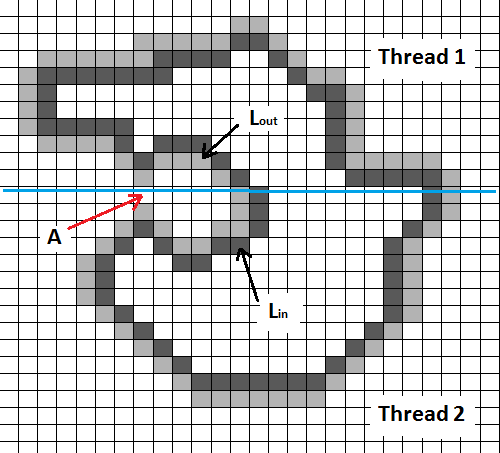
\includegraphics[width=0.6\textwidth]{./imagenes/mismoVecino}
 	\caption{Ejemplo de condici�n de carrera al querer a�adir un punto vecino en com�n a puntos tratados por distintos \textit{threads}}	
 	\label{mismoVecino}
 \end{figure}

\subsection{Primera implementaci�n}

En esta secci�n se explican las caracter�sticas de la primera implementaci�n paralela realizada siguiendo el an�lisis del anterior apartado. As� pues, cada ciclo quedar� estructurado como se ve en la figura \ref{1-Imple}. Las nuevas caracter�sticas son de color rojo y se han marcado con un asterisco(*). 

 \begin{figure}[H]
 	\captionsetup{justification=centering}
 	\centering
 	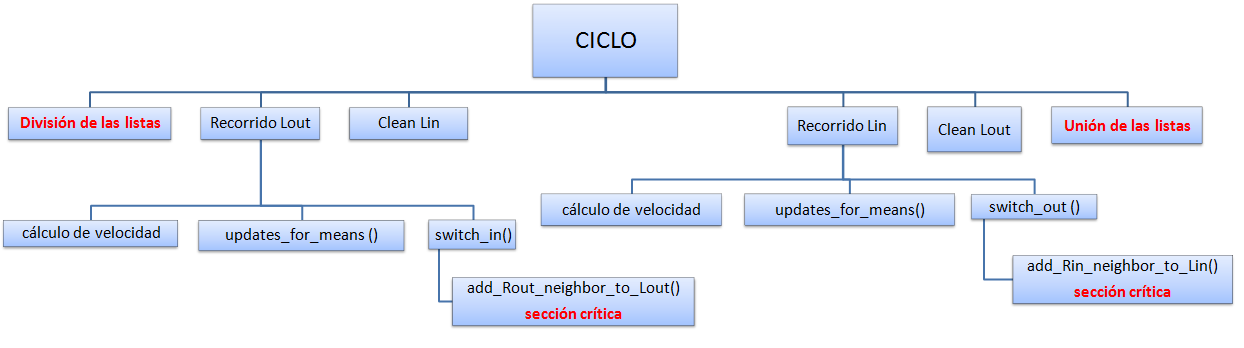
\includegraphics[width=1.2\textwidth]{./imagenes/1-Imple}
 	\caption{Esquema de la primera implementaci�n}	
 	\label{1-Imple}
 \end{figure}

En esta primera implementaci�n se invirti� mucho tiempo ya que los cambios realizados fueron muchos. Se ir� paso a paso comentando las caracter�sticas de cada cambio, as� como la raz�n por la que se llevo a cabo dicho cambio.

\subsubsection{Lista enlazada}

Muchos han sido los cambios realizados en comparaci�n con la implementaci�n de lista enlazada creada en el trabajo Ofeli. Todos los cambios aqu� realizados han tenido como objetivo minimizar el coste operacional de las operaciones necesarias para realizar la paralelizaci�n. 

\begin{enumerate}
	\item Se ha insertado en cada nodo un puntero hacia el elemento anterior, es decir, se ha creado una lista doblemente ligada. 
	\item La modificaci�n anterior ha dado pie a crear un apuntador al final de la lista, un \textit{tail}.
	\item Se ha convertido el tiempo de la ejecuci�n de la funci�n size() en orden constante en lugar de la implementaci�n computacionalmente lineal (al n�mero de elementos de la lista) que estaba.
	\item Otras modificaciones que no influyen en la implementaci�n paralela.
\end{enumerate}

\subsubsection{Divisi�n de la lista}

Las listas $L_{out}$ y $L_{in}$ se dividen en un n�mero de trozos o sublistas igual al n�mero de \textit{threads} de manera que cada uno tenga la parte de la lista original con la que trabajar�. 

Al inicio del programa, despu�s de inicializar las dos listas con el contorno definido manualmente, se crean tantos punteros o apuntadores como \textit{threads} vayan a trabajar en la ejecuci�n. Cada puntero se coloca apuntando al primer elemento que tratar� cada \textit{thread}, es decir, suponiendo que tenemos 80 elementos a repartir entre cuatro \textit{threads}, el primer puntero apuntar� al primer elemento, ya que ser� el primer elemento a tratar por el primer \textit{thread}, el segundo puntero apuntar� al vig�simo primer elemento y as� sucesivamente. V�ase la figura \ref{divisionLista1} para ver un ejemplo de ello. Esta primera recolocaci�n de los \textit{heads} de cada \textit{thread} se realiza en tiempo lineal al n�mero de elementos en las listas, sin embargo, esta operaci�n s�lo se realiza en la preparaci�n de la evoluci�n y por lo tanto, una sola vez. 

 \begin{figure}[H]
 	\captionsetup{justification=centering}
 	\centering
 	\includegraphics[width=1\textwidth]{./imagenes/divisionLista1}
 	\caption{Esquema de la colocaci�n de los \textit{heads} de trozo de lista a crear}	
 	\label{divisionLista1}
 \end{figure}
 
 
Por lo tanto, se accede en un orden constante a cada elemento \textit{head} creado, se establecen los \textit{tails} de las sublistas accediendo al anterior elemento de estos \textit{heads}, se establecen los tama�os de cada sublista (posible conociendo la posici�n de cada \textit{tail} y llevando una cuenta) y se <<rompen>> los enlaces con sus anteriores elementos de manera que se separen por completo las sublistas. Todo ello es posible gracias a las modificaciones realizadas en la implementaci�n de la lista ligada. V�ase la figura \ref{divisionLista2} para ver un ejemplo de todo ello. 

 \begin{figure}[H]
 	\captionsetup{justification=centering}
 	\centering
 	\includegraphics[width=1\textwidth]{./imagenes/divisionLista2}
 	\caption{Ejemplo de creaci�n de cada sublista usando los \textit{heads} establecidos}	
 	\label{divisionLista2}
 \end{figure} 
 
 
\subsubsection{Uni�n de las sublistas} 

Siguiendo el procedimiento inverso a la divisi�n de las listas se realiza la uni�n. En este caso, sabiendo los \textit{heads} y los \textit{tails} de cada sublista, se vuelve a crear la uni�n entre ellas, m�s concretamente, entre el \textit{tail} y el \textit{head} de la siguiente lista. El tama�o de la lista completa ser� la suma de los tama�os de todas las sublistas. V�ase la figura \ref{unionLista1} como explicaci�n de ello.

 \begin{figure}[H]
 	\captionsetup{justification=centering}
 	\centering
 	\includegraphics[width=1\textwidth]{./imagenes/unionLista1}
 	\caption{Ejemplo de uni�n de cada sublista usando los \textit{heads} y \textit{tails} de cada una}	
 	\label{unionLista1}
 \end{figure} 
 
Al realizar esta uni�n, tambi�n se aprovecha a reinicializar los \textit{heads} que se utilizar�n en la siguiente divisi�n de la lista. Los \textit{heads} se inicializar�n previamente como los \textit{heads} de cada sublista. N�tese que estos \textit{heads} se habr�n posicionado muy cerca de la posici�n �ptima, ya que habitualmente todas las zonas del contorno tienden a expandirse por igual. No obstante, se realiza un centrado de cada \textit{head}, es decir, se mueve el puntero hasta la posici�n exacta en la que debe estar, si es que no lo est�, realizando la divisi�n del n�mero de puntos entre el n�mero de \textit{thread} de la ejecuci�n. Los \textit{tails} no har�n falta establecerlos ya que se posicionan en la divisi�n de las listas. V�ase la figura \ref{unionLista2} como explicaci�n de ello. El n�mero de operaciones a realizar comparadas con el n�mero de puntos en la lista es peque�o.

 \begin{figure}[H]
 	\captionsetup{justification=centering}
 	\centering
 	\includegraphics[width=1\textwidth]{./imagenes/unionLista2}
 	\caption{Ejemplo de uni�n de cada sublista usando los \textit{heads} y \textit{tails} de cada una}	
 	\label{unionLista2}
 \end{figure}
 
 
 
 \subsubsection{Secciones cr�ticas} 
 
 Las secciones cr�ticas a realizar para resolver la condici�n de carrera se han establecido en las funciones de a�adir un vecino del punto que se cambia de una lista a otra. Se ha seguido un esquema \textit{Test and Test-and-set} para minimizar la contenci�n de la secci�n cr�tica ya que se realiza antes la condici�n que se debe de hacer en la secci�n cr�tica antes de entrar a �sta.
 
 A continuaci�n se presenta el c�digo de la secci�n cr�tica.


\subsubsection{C�digo}

\begin{lstlisting}
void ActiveContour::add_Rout_neighbor_to_Lout(int neighbor_offset,int tid)
{
	//Test, test and set
	if( phi[neighbor_offset] == 3 ) // exterior value
	{
		#pragma omp critical
		{
			if( phi[neighbor_offset] == 3 ) // exterior value
			{
				phi[neighbor_offset] = 1; // outside boundary value
	
				Splited_Lout[tid]->push_front(neighbor_offset);	
			}
		}
	}	
return;}

void ActiveContour::add_Rin_neighbor_to_Lin(int neighbor_offset,int tid)
{
	//Test, test and set
	if( phi[neighbor_offset] == -3 ) // interior value
	{
		#pragma omp critical
		{
			if( phi[neighbor_offset] == -3 ) // interior value
			{
				phi[neighbor_offset] = -1; // inside boundary value
			
				Splited_Lin[tid]->push_front(neighbor_offset);
			}
		}
	}	
return;}	
\end{lstlisting}

 
\subsection{Rendimiento}
 
Realizada la primera implementaci�n, llega la hora de comprobar su rendimiento y ver la mejora obtenida respecto a la versi�n serie. En estas primeras pruebas se ha utilizado �nicamente una imagen de tama�o 3000x2800 y que es exactamente la que se muestra en la figura \ref{ejemplo4}.

Las pruebas realizadas han sido en un ordenador de la Universidad del Pa�s Vasco. Este ordenador tiene una arquitectura SMP, con una memoria principal de 64GB y dispone de cuatro procesadores \textit{AMD Opteron(tm) Processor 6168} los cuales tienen doce \textit{cores} que trabajan a 1900 MHz. Por lo tanto, se disponen de 48 \textit{cores} para poder realizar las pruebas. Tambi�n se ha considerado a�adir que se ha tenido que separar la parte gr�fica del trabajo original de Ofeli y extraer el algoritmo de evoluci�n para poder realizar las pruebas. 

La compilaci�n se ha realizado con el compilador gcc (versi�n 4.6.3) con la siguiente l�nea de comandos:

\

\quad \quad \textbf{g++ main.cpp activecontour.cpp ac\_withoutedges.cpp -o prueba}

\quad \quad	\textbf{-O3 -fopenmp -Dcimg\_use\_png -lpng -lz -Dcimg\_display=0}

\

Mientras no se diga lo contrario, todas las ejecuciones se realizar�n en la misma m�quina y los tiempos de todas las tablas que aparezcan ser�n la media de cinco ejecuciones. A esta primera implementaci�n se le nombrar� como <<secci�n critica normal>>.


\begin{table}[h]
	\small
	\centering
	\captionsetup{justification=centering}
	\begin{tabular}{cccccccc}
		\hline
		\multicolumn{1}{|c|}{{\bf N�mero de threads}} & \multicolumn{1}{c|}{{\bf Serie}} & \multicolumn{1}{c|}{{\bf 2}} & \multicolumn{1}{c|}{{\bf 4}} & \multicolumn{1}{c|}{{\bf 8}} & \multicolumn{1}{c|}{{\bf 16}} & \multicolumn{1}{c|}{{\bf 32}} & \multicolumn{1}{c|}{{\bf 48}} \\ \hline
		\multicolumn{1}{|c|}{{\bf Tiempo (s)}}           & \multicolumn{1}{c|}{16,52}      & \multicolumn{1}{c|}{11,63}  & \multicolumn{1}{c|}{7,80}   & \multicolumn{1}{c|}{9,38}   & \multicolumn{1}{c|}{14,37}   & \multicolumn{1}{c|}{27,66}   & \multicolumn{1}{c|}{31,37}   \\ \hline
		\multicolumn{1}{l}{}                         & \multicolumn{1}{l}{}             & \multicolumn{1}{l}{}         & \multicolumn{1}{l}{}         & \multicolumn{1}{l}{}         & \multicolumn{1}{l}{}          & \multicolumn{1}{l}{}          & \multicolumn{1}{l}{}          \\ \hline
		\multicolumn{1}{|c|}{{\bf Speed-up}}         & \multicolumn{1}{c|}{1,00}        & \multicolumn{1}{c|}{1,42}    & \multicolumn{1}{c|}{2,12}    & \multicolumn{1}{c|}{1,76}    & \multicolumn{1}{c|}{1,15}     & \multicolumn{1}{c|}{0,60}     & \multicolumn{1}{c|}{0,53}     \\ \hline
		{\bf }                                       &                                  &                              &                              &                              &                               &                               &                               \\ \hline
		\multicolumn{1}{|c|}{{\bf Eficiencia}}       & \multicolumn{1}{c|}{100,00\%}    & \multicolumn{1}{c|}{71,03\%} & \multicolumn{1}{c|}{52,98\%} & \multicolumn{1}{c|}{22,02\%} & \multicolumn{1}{c|}{7,19\%}   & \multicolumn{1}{c|}{1,87\%}   & \multicolumn{1}{c|}{1,10\%}   \\ \hline
	\end{tabular}
	\caption{Rendimiento de las ejecuciones de la primera implementaci�n paralela}
\end{table}	


\begin{figure}[H]
 	\captionsetup{justification=centering}
 	\centering
 	\includegraphics[width=.7\textwidth]{./imagenes/grafico1Imple}
 	\caption{Gr�fica de los tiempos de ejecuci�n de la primera implementaci�n paralela}	
 	\label{grafico1Imple}
\end{figure}

Como se puede observar en la figura \ref{grafico1Imple}, esta primera implementaci�n s�lo escala bien hasta los cuatro \textit{cores}. 

\subsubsection{Conclusi�n}

Se analizan los tiempos de ejecuci�n y se comprueba que, efectivamente, el cuello de botella est� en el acceso a la secci�n cr�tica. V�ase el desglose del tiempo de ejecuci�n (2 \textit{cores}) de un ciclo en la tabla \ref{tablaConclusiones1}. Aqu� se puede observar que la mayor�a del tiempo se pierde en realizar los bucles 1 y 2, es decir, donde est�n las funciones con la secciones cr�ticas. Esto sucede ya que �sta se hace pr�cticamente siempre, debido a que el contorno suele tender a expandirse, y puede que se repita varias veces por cada punto, al realizarse por cada nuevo vecino. Por otro lado, la ejecuci�n es �nicamente con dos \textit{cores}, por lo que la contenci�n de la secci�n cr�tica ser� mayor con m�s \textit{cores}, raz�n por la que esta primera implementaci�n no escala bien.

\begin{table}[H]
	\centering
	\small
	\captionsetup{justification=centering}
	\begin{tabular}{c|c|c|c|c|c|c|c}
		\cline{2-8}
		\multicolumn{1}{l|}{}                          & {\bf \begin{tabular}[c]{@{}c@{}}Divisi�n\\   listas\end{tabular}} & {\bf  \begin{tabular}[c]{@{}c@{}}1�\\   bucle\end{tabular}} & {\bf \begin{tabular}[c]{@{}c@{}}Clean\\   Lin\end{tabular}} & {\bf  \begin{tabular}[c]{@{}c@{}}2�\\   bucle\end{tabular}} & {\bf \begin{tabular}[c]{@{}c@{}}Clean\\   Lout\end{tabular}} & {\bf \begin{tabular}[c]{@{}c@{}}Uni�n\\   listas\end{tabular}} & \multicolumn{1}{c|}{{\bf \begin{tabular}[c]{@{}c@{}}POR\\   CICLO\end{tabular}}} \\ \hline
		\multicolumn{1}{|c|}{{\bf Serie}}              & 0,0                  & 0,0127       & 0,008         & 0,0145       & 0,0071         & 0,0                                                               & \multicolumn{1}{c|}{0,043}         \\ \hline
		\multicolumn{1}{|c|}{{\bf \begin{tabular}[c]{@{}c@{}}�ptimo 2\\   threads\end{tabular}}}   & 0,0                  & 0,0063       & 0,0040        & 0,0072       & 0,0035         & 0,0                                                              & \multicolumn{1}{c|}{0,0215}        \\ \hline
		\multicolumn{1}{|c|}{{\bf \begin{tabular}[c]{@{}c@{}}Paralelo 2\\   threads\end{tabular}}} & 0,0                  & 0,0093       & 0,0041        & 0,0109       & 0,0038         & 0,0                                                               & \multicolumn{1}{c|}{0,0281}        \\ \hline
		\multicolumn{1}{|c|}{{\bf Sobrecoste}}           & 0,0\%                    & 46,0\%         & 2,1\%           & 51,3\%         & 8,6\%            & 0,0\%                                                                 & \multicolumn{1}{l}{}                 \\ \cline{1-7}
	\end{tabular}
	\caption{Desglose de tiempos (s) de un ciclo del algoritmo con una ejecuci�n paralela con dos \textit{cores} de la primera implementaci�n}		
	\label{tablaConclusiones1}
\end{table}


\section{Primer paso de mejora: segunda implementaci�n}

Concluido ya que el problema est� en la secci�n cr�tica se intenta reducir las operaciones dentro de �sta reduciendo as� el tiempo que cada \textit{thread} est� dentro de ella. La <<secci�n cr�tica mejorada>> tendr� �nicamente dos asignaciones, reduciendo considerablemente el tiempo dentro de ella. Se utilizar� un \textit{flag} para saber qu� \textit{thread} ha sido el que ha entrado a la secci�n cr�tica para posteriormente hacer la operaci�n correspondiente. En este caso obviaremos la segunda funci�n ya que tiene las mismas caracter�sticas que la primera.

\subsubsection{C�digo}

\begin{lstlisting}

 void ActiveContour::add_Rout_neighbor_to_Lout(int neighbor_offset,int tid)
 {
 	bool flag = false;
 	
 	if( phi[neighbor_offset] == 3 ) // exterior value
 	{
 		#pragma omp critical
 		{
 			if( phi[neighbor_offset] == 3 ) // exterior value
 			{
 				phi[neighbor_offset] = 1; // outside boundary value
 				flag = true;
 			}
 		}
 		if(flag)  Splited_Lout[tid]->push_front(neighbor_offset);
 	} 	
 	return; 
 }
 	
\end{lstlisting}

\subsection{Rendimiento}

\begin{table}[H]
	\small
	\centering
	\captionsetup{justification=centering}
	\begin{tabular}{cccccccc}
		\hline
		\multicolumn{1}{|c|}{{\bf N�m. \textit{threads}}} & \multicolumn{1}{c|}{{\bf Serie}} & \multicolumn{1}{c|}{{\bf 2}} & \multicolumn{1}{c|}{{\bf 4}} & \multicolumn{1}{c|}{{\bf 8}} & \multicolumn{1}{c|}{{\bf 16}} & \multicolumn{1}{c|}{{\bf 32}} & \multicolumn{1}{c|}{{\bf 48}} \\ \hline
		\multicolumn{1}{|c|}{{\bf Tiempo (s)}}           & \multicolumn{1}{c|}{16,52}      & \multicolumn{1}{c|}{10,74}  & \multicolumn{1}{c|}{6,58}   & \multicolumn{1}{c|}{5,42}   & \multicolumn{1}{c|}{3,68}    & \multicolumn{1}{c|}{6,02}    & \multicolumn{1}{c|}{6,79}    \\ \hline
		\multicolumn{1}{l}{}                         & \multicolumn{1}{l}{}             & \multicolumn{1}{l}{}         & \multicolumn{1}{l}{}         & \multicolumn{1}{l}{}         & \multicolumn{1}{l}{}          & \multicolumn{1}{l}{}          & \multicolumn{1}{l}{}          \\ \hline
		\multicolumn{1}{|c|}{{\bf Speed-up}}         & \multicolumn{1}{c|}{1,00}        & \multicolumn{1}{c|}{1,54}    & \multicolumn{1}{c|}{2,51}    & \multicolumn{1}{c|}{3,05}    & \multicolumn{1}{c|}{4,49}     & \multicolumn{1}{c|}{2,74}     & \multicolumn{1}{c|}{2,43}     \\ \hline
		{\bf }                                       &                                  &                              &                              &                              &                               &                               &                               \\ \hline
		\multicolumn{1}{|c|}{{\bf Eficiencia}}       & \multicolumn{1}{c|}{100,0\%}    & \multicolumn{1}{c|}{76,9\%} & \multicolumn{1}{c|}{62,8\%} & \multicolumn{1}{c|}{38,1\%} & \multicolumn{1}{c|}{28,1\%}  & \multicolumn{1}{c|}{8,6\%}   & \multicolumn{1}{c|}{5,1\%}   \\ \hline
	\end{tabular}
	\caption{Rendimiento obtenido de las ejecuciones de la segunda implementaci�n paralela}
\end{table}




\begin{figure}[H]
	\captionsetup{justification=centering}
	\centering
	\includegraphics[width=.8\textwidth]{./imagenes/grafico2Imple}
	\caption{Gr�fica de los tiempos de ejecuci�n de la primera y segunda implementaci�n}	
	\label{grafico2Imple}
\end{figure}

Como se puede ver en el gr�fico \ref{grafico2Imple} la mejora es bastante notable. Esto se debe a que se ha reducido notablemente la contenci�n entre los \textit{threads} al no tener pr�cticamente operaciones a realizar dentro de la secci�n cr�tica. El tiempo de ejecuci�n del sistema se reduce hasta los 16 cores.

\


\subsubsection{Conclusi�n}

A pesar de haber mejorado mucho los tiempos el resultado no sigue siendo �ptimo del todo ya que la implementaci�n escala poco a poco hasta los 16 \textit{threads} y luego el tiempo va aumentado. Hay que intentar reducir a�n m�s la contenci�n de alguna manera. Analizando un poco m�s a detalle, la secci�n cr�tica se realiza para cualquier vecino que se quiera a�adir despu�s de haber expandido o contra�do un punto. Es decir, que no importa la localizaci�n de los puntos que se est�n tratando, habr� colisi�n en la secci�n cr�tica. En realidad, la secci�n cr�tica se puso para evitar que se pudieran a�adir varios puntos vecinos a la vez. �Hay alguna manera de realizar secciones cr�ticas dependientes del punto? Ser�a la pregunta clave a responder para poder resolver el problema. 

\section{Segundo paso de mejora: tercera implementaci�n}

Buscando alguna manera de realizar secciones cr�ticas dependiente del punto se deciden usar sem�foros o \textit{locks} en ingl�s. Se podr�a tener una matriz de \textit{locks} de la misma dimensi�n que la imagen y cada vez que se vaya a trabajar con un punto cerrar el \textit{lock} que le pertenece. El problema de esta idea de tener un \textit{lock} para cada p�xel, en una imagen de 3000x2800, ser�a la cantidad de memoria y la complejidad de gesti�n de �stos, ya que el n�mero de \textit{locks} necesarios ser�a muy elevado. Como alternativa y buscando una soluci�n de compromiso se ha implementado un esquema de \textit{locks} por zonas. En vez de tener un \textit{lock} para cada punto se podr�a tener un n�mero de \textit{locks} no muy grande para bloquear cierta zona de la imagen. 

\begin{figure}[H]
	\captionsetup{justification=centering}
	\centering
	\includegraphics[width=.7\textwidth]{./imagenes/mallaLocks}
	\caption{Ejemplo de una malla de cuatro locks de establecidos en forma rectangular}	
	\label{mallaLocks}
\end{figure}

En la imagen \ref{mallaLocks} se puede observar un ejemplo de una malla de \textit{locks} en la n�mero de \textit{locks} establecido es 4 y tiene una forma rectangular. El n�mero de �ptimo de locks a establecer ser� lo que se trabaje en esta tercera implementaci�n. Adem�s, el lector podr�a pensar que se pueden realizar distintas figuras geom�tricas en la creaci�n de la estructura de \textit{locks}, aunque esta opci�n no se realizar� en este proyecto ya que la estrategia de distribuci�n de los puntos en las sublistas se realiza recorriendo la matriz por filas, lo que significa que los rect�ngulos dar�n una mejor respuesta temporal ya que habr� poca colisi�n entre los \textit{threads}.

\subsubsection{C�digo}

\begin{lstlisting}
void ActiveContour::add_Rout_neighbor_to_Lout(int neighbor_offset,int tid)
{
	bool flag = false;	
	
	if( phi[neighbor_offset] == 3 ) // exterior value
	{
		int lockNumber = ( (neighbor_offset/img_width) *numLocks)/img_height;
					
		omp_set_lock(&(locks[lockNumber]));	
					
		if( phi[neighbor_offset] == 3 ) // exterior value
		{
			phi[neighbor_offset] = 1; // outside boundary value
			flag = true;
		}	
		
		omp_unset_lock(&(locks[lockNumber]));	
		
		if(flag)  Splited_Lout[tid]->push_front(neighbor_offset);
	}
	return;	
}
\end{lstlisting}


\subsection{Rendimiento}


\begin{table}[H]
	\centering
	\captionsetup{justification=centering}
	\begin{tabular}{lc|c|c|c|c|c|c|lcccl}
		\cline{3-8}
		& \multicolumn{1}{l|}{} & \multicolumn{6}{c|}{{\bf Locks}}                              &                       & \multicolumn{1}{l}{}          & \multicolumn{1}{l}{}  & \multicolumn{1}{l}{}            &  \\ \cline{3-8} \cline{10-10} \cline{12-12}
		&                       & {\bf 4} & {\bf 8} & {\bf 16} & {\bf 24} & {\bf 32} & {\bf 50} & \multicolumn{1}{l|}{} & \multicolumn{1}{c|}{{\bf su}} & \multicolumn{1}{c|}{} & \multicolumn{1}{c|}{{\bf Efi.}} &  \\ \cline{1-8} \cline{10-10} \cline{12-12}
		\multicolumn{1}{|l|}{\multirow{13}{*}{{\bf \rotatebox[origin=c]{90}{THREADS}}}} & {\bf 1}               & 16,69   & 16,64   & 16,63    & 16,61    & 16,79    & 16,73    & \multicolumn{1}{l|}{} & \multicolumn{1}{c|}{-}        & \multicolumn{1}{c|}{} & \multicolumn{1}{c|}{-}          &  \\ \cline{2-8} \cline{10-10} \cline{12-12}
		\multicolumn{1}{|l|}{}                                & {\bf 2}               & 10,49   & 10,64   & 10,35    & 10,52    & 10,35    & 10,33    & \multicolumn{1}{l|}{} & \multicolumn{1}{c|}{1,59}     & \multicolumn{1}{c|}{} & \multicolumn{1}{c|}{79,6\%}     &  \\ \cline{2-8} \cline{10-10} \cline{12-12}
		\multicolumn{1}{|l|}{}                                & {\bf 4}               & 6,79    & 7,03    & 6,86     & 6,85     & 6,73     & 6,60     & \multicolumn{1}{l|}{} & \multicolumn{1}{c|}{2,46}     & \multicolumn{1}{c|}{} & \multicolumn{1}{c|}{61,5\%}     &  \\ \cline{2-8} \cline{10-10} \cline{12-12}
		\multicolumn{1}{|l|}{}                                & {\bf 8}               & 4,22    & 5,73    & 5,72     & 5,42     & 5,44     & 5,40     & \multicolumn{1}{l|}{} & \multicolumn{1}{c|}{3,96}     & \multicolumn{1}{c|}{} & \multicolumn{1}{c|}{49,5\%}     &  \\ \cline{2-8} \cline{10-10} \cline{12-12}
		\multicolumn{1}{|l|}{}                                & {\bf 16}              & 3,99    & 3,93    & 4,89     & 3,26     & 4,87     & 4,84     & \multicolumn{1}{l|}{} & \multicolumn{1}{c|}{4,18}     & \multicolumn{1}{c|}{} & \multicolumn{1}{c|}{26,1\%}     &  \\ \cline{2-8} \cline{10-10} \cline{12-12}
		\multicolumn{1}{|l|}{}                                & {\bf 20}              & 3,29    & 3,87    & 3,88     & 3,19     & 3,89     & 3,89     & \multicolumn{1}{l|}{} & \multicolumn{1}{c|}{5,08}     & \multicolumn{1}{c|}{} & \multicolumn{1}{c|}{25,4\%}     &  \\ \cline{2-8} \cline{10-10} \cline{12-12}
		\multicolumn{1}{|l|}{}                                & {\bf 24}              & 2,95    & 3,28    & 3,29     & 3,32     & 3,30     & 3,29     & \multicolumn{1}{l|}{} & \multicolumn{1}{c|}{5,65}     & \multicolumn{1}{c|}{} & \multicolumn{1}{c|}{23,5\%}     &  \\ \cline{2-8} \cline{10-10} \cline{12-12}
		\multicolumn{1}{|l|}{}                                & {\bf 28}              & 3,03    & 2,96    & 2,93     & 2,92     & 2,96     & 2,93     & \multicolumn{1}{l|}{} & \multicolumn{1}{c|}{5,52}     & \multicolumn{1}{c|}{} & \multicolumn{1}{c|}{19,7\%}     &  \\ \cline{2-8} \cline{10-10} \cline{12-12}
		\multicolumn{1}{|l|}{}                                & {\bf 32}              & 2,85    & 2,72    & 2,80     & 2,70     & 3,00     & 2,80     & \multicolumn{1}{l|}{} & \multicolumn{1}{c|}{5,86}     & \multicolumn{1}{c|}{} & \multicolumn{1}{c|}{18,3\%}     &  \\ \cline{2-8} \cline{10-10} \cline{12-12}
		\multicolumn{1}{|l|}{}                                & {\bf 36}              & 3,74    & 3,81    & 3,29     & 3,48     & 2,85     & 3,28     & \multicolumn{1}{l|}{} & \multicolumn{1}{c|}{4,46}     & \multicolumn{1}{c|}{} & \multicolumn{1}{c|}{12,4\%}     &  \\ \cline{2-8} \cline{10-10} \cline{12-12}
		\multicolumn{1}{|l|}{}                                & {\bf 40}              & 4,12    & 4,06    & 3,79     & 3,98     & 3,85     & 3,81     & \multicolumn{1}{l|}{} & \multicolumn{1}{c|}{4,05}     & \multicolumn{1}{c|}{} & \multicolumn{1}{c|}{10,1\%}     &  \\ \cline{2-8} \cline{10-10} \cline{12-12}
		\multicolumn{1}{|l|}{}                                & {\bf 44}              & 4,00    & 4,06    & 4,05     & 3,83     & 3,75     & 3,74     & \multicolumn{1}{l|}{} & \multicolumn{1}{c|}{4,18}     & \multicolumn{1}{c|}{} & \multicolumn{1}{c|}{9,5\%}      &  \\ \cline{2-8} \cline{10-10} \cline{12-12}
		\multicolumn{1}{|l|}{}                                & {\bf 48}              & 3,91    & 3,91    & 3,77     & 3,68     & 3,82     & 3,66     & \multicolumn{1}{l|}{} & \multicolumn{1}{c|}{4,27}     & \multicolumn{1}{c|}{} & \multicolumn{1}{c|}{8,9\%}      &  \\ \cline{1-8} \cline{10-10} \cline{12-12}
	\end{tabular}
	\caption{Tiempos de ejecuci�n (s),  eficiencia y \textit{speed-ups} (su) obtenidos con distintas combinaciones de \textit{threads} y \textit{locks} en la tercera implementaci�n paralela}
\end{table}

\begin{figure}[H]
	\captionsetup{justification=centering}
	\centering
	\includegraphics[width=0.8\textwidth]{./imagenes/grafico3Imple}
	\caption{Gr�fico de los resultados obtenidos en este tercera implementaci�n}
	\label{Implementacion3}
\end{figure}

Como se puede observar en la figura \ref{Implementacion3} se ha mejorado a�n m�s la respuesta temporal, escala bien hasta los 32 \textit{threads} en vez de hasta los 16 que se consegu�an con la anterior implementaci�n (v�ase la figura \ref{grafico2Imple}). Las ejecuciones m�s r�pidas se logran con la combinaci�n de 32 \textit{threads} y con 24 \textit{locks}, teniendo un resultado de 2,7 segundos. 

Por otro lado, tambi�n se han realizado pruebas con la primera implementaci�n, es decir, con la <<secci�n cr�tica normal>> para analizar el efecto de la reducci�n de la contenci�n mediante la soluci�n de \textit{locks} distribuidos en dicha implementaci�n. Esto se refiere a que la secci�n la crear�n los \textit{locks} pero lo que hay dentro ser� lo que hab�a en la implementaci�n de la <<secci�n cr�tica normal>>. Los resultados son los que se muestran en el gr�fico \ref{grafico3-2Imple}. Como se puede observar el tiempo obtenido es pr�cticamente el conseguido con la �ltima implementaci�n realizada. Esto quiere decir que el problema de todo ello era la contenci�n que hab�a con todos los \textit{threads} y no importa tanto el tiempo que se pasa dentro de la secci�n cr�tica. Sin embargo, tambi�n ah� que decir que con la implementaci�n de la <<secci�n cr�tica normal>> son necesarios m�s \textit{locks} para evitar esa contenci�n entre los \textit{threads} ya que la secci�n cr�tica es m�s larga.

\begin{figure}[H]
	\captionsetup{justification=centering}
	\centering
	\includegraphics[width=.9\textwidth]{./imagenes/grafico3-2Imple}
	\caption{Gr�fica de los tiempos de ejecuci�n con los \textit{locks} y la estructura de la <<secci�n cr�tica normal>>}	
	\label{grafico3-2Imple}
\end{figure}


\subsubsection{Conclusi�n}

Ya que los resultados obtenidos con la �ltima implementaci�n y la primera son parecidos no se podr� reducir mucho m�s el tiempo en cuanto a la contenci�n, ya que parece que a partir de cierto n�mero de \textit{locks} �sta desaparece. As� pues, la reducci�n tendr�a que hacerse por otra v�a, o bien intentar reducir el tiempo que se realiza en paralelo o entrar en m�s detalle como la compartici�n falsa en la memoria cach� que pudiera haber con ciertas variables de la implementaci�n. El propio tiempo de gesti�n de los \textit{locks}, la compartici�n falsa en cach� que pudiera haber con ciertas variables, la gesti�n de la secci�n paralela y la divisi�n y uni�n de las listas parece que a�aden en total un \textit{overhead} que se ha decidido dejar fuera del �mbito de este proyecto. 








\chapter{Experimentaci�n}

En este cap�tulo mostraremos el rendimiento de la mejor versi�n implementada, la tercera versi�n, aquella con la <<secci�n critica mejorada>> y haciendo uso de la malla de \textit{locks} con mas detalle. En las anteriores presentaciones de los rendimientos de las distintas implementaciones se ha utilizado un tipo de imagen, tama�o de esta e inicializaci�n inicial del contorno. En este apartado realizaremos pruebas m�s completas, combinando distintos factores para ver mas detalladamente el comportamiento de la mejor versi�n de la paralelizaci�n. Adem�s, se podr� llegar a concluir que tipo de combinaci�n beneficia a la evoluci�n del contorno en cierto tipo de im�genes.

Se ha decidido probar 3 tipos de im�genes diferentes, con varios tama�os de estas, varios tama�os de las mallas de \textit{locks} y varios \textit{threads}. En la figura \ref{tiposImagenes} se puede observar los tres tipos de im�genes diferentes que se utilizar�n en la realizaci�n de dichas pruebas.


\begin{figure}[H]
	\centering	
	\captionsetup{justification=centering}	
	\begin{center}
		\begin{subfigure}[t]{2.5in}
			\centering
			\includegraphics[width=.7\textwidth]{./imagenes/buena1}
			\subcaption{}\label{buena1}
		\end{subfigure}
		\begin{subfigure}[t]{2.5in}
			\centering
			\includegraphics[width=.8\textwidth]{./imagenes/ejemplo2}	
			\subcaption{}\label{buena2}
		\end{subfigure}
		\begin{subfigure}[t]{2.5in}
			\centering
			\includegraphics[width=.8\textwidth]{./imagenes/buena3}	
			\subcaption{}\label{buena3}
		\end{subfigure}
	\end{center}
	\caption{Tipos de im�genes con las que se realizar�n las pruebas completas de la tercera implementaci�n}
	\label{tiposImagenes}
\end{figure} 


\section{Primera imagen}

La primera imagen a probar ser� la imagen \ref{buena1} y a continuaci�n se presentan los resultados de las ejecuciones con diferentes tama�os de la imagen.

\subsubsection{500x500}

\begin{table}[H]
	\centering
	\begin{tabular}{|c|c|c|c|c|c|c|}
		\hline
		{\bf \backslashbox{Threads}{Locks}}   & {\bf 4} & {\bf 8} & {\bf 16} & {\bf 24} & {\bf 32} & {\bf 50} \\ \hline
		{\bf 1}  & 2,01    & 2,03    & 2,03     & 2,04     & 2,04     & 2,03     \\ \hline
		{\bf 2}  & 1,34    & 1,37    & 1,37     & 1,34     & 1,35     & 1,35     \\ \hline
		{\bf 4}  & 1,00    & 0,96    & 0,96     & 0,97     & 0,96     & 0,95     \\ \hline
		{\bf 8}  & 0,62    & 0,91    & 0,91     & 0,80     & 0,88     & 0,90     \\ \hline
		{\bf 16} & 0,62    & 0,56    & 0,56     & 0,48     & 0,74     & 0,70     \\ \hline
		{\bf 20} & 0,53    & 0,64    & 0,64     & 0,50     & 0,67     & 0,60     \\ \hline
		{\bf 24} & 0,43    & 0,52    & 0,52     & 0,56     & 0,56     & 0,49     \\ \hline
		{\bf 28} & 0,47    & 0,43    & 0,43     & 0,45     & 0,43     & 0,47     \\ \hline
		{\bf 32} & 0,42    & 0,40    & 0,40     & 0,39     & 0,38     & 0,39     \\ \hline
		{\bf 36} & 0,44    & 0,37    & 0,37     & 0,35     & 0,34     & 0,36     \\ \hline
		{\bf 40} & 0,44    & 0,32    & 0,32     & 0,31     & 0,32     & 0,32     \\ \hline
		{\bf 44} & 0,45    & 0,35    & 0,35     & 0,31     & 0,31     & 0,30     \\ \hline
		{\bf 48} & 0,45    & 0,36    & 0,36     & 0,33     & 0,34     & 0,37     \\ \hline
	\end{tabular}
	\captionsetup{justification=centering}	
	\caption{Tiempos de ejecuci�n de la imagen \ref{buena1} con un tama�o de 500x500}
	\label{img1-500}	
\end{table}

Como se puede observar en la tabla \ref{img1-500} los mejores tiempos se consiguen con 40 y 44 \textit{threads} y a partir de los 24 \textit{locks}. El menor tiempo que se consigue es de 0,3 segundos, con un \textit{speed-up} de 6,7 y una eficiencia del 15,1\%.

\begin{figure}[H]
	\captionsetup{justification=centering}
	\centering
	\includegraphics[width=.7\textwidth]{./imagenes/graf1-500}
	\caption{Gr�fica de los tiempos de ejecuci�n de la imagen \ref{buena1} con un tama�o de 500x500}	
	\label{graf1-500}
\end{figure}

\subsubsection{1500x1500}


\begin{table}[H]
	\centering
	\begin{tabular}{|c|c|c|c|c|c|c|}
		\hline
		{\bf \backslashbox{Threads}{Locks}}   & {\bf 4} & {\bf 8} & {\bf 16} & {\bf 24} & {\bf 32} & {\bf 50} \\ \hline
		{\bf 1}  & 14,88   & 14,91   & 14,92    & 14,87    & 14,92    & 14,90    \\ \hline
		{\bf 2}  & 8,52    & 8,54    & 8,42     & 8,54     & 8,52     & 8,50     \\ \hline
		{\bf 4}  & 5,96    & 5,96    & 5,82     & 5,88     & 5,88     & 5,88     \\ \hline
		{\bf 8}  & 3,34    & 4,89    & 4,87     & 4,80     & 4,80     & 4,80     \\ \hline
		{\bf 16} & 3,45    & 3,40    & 4,27     & 2,58     & 4,28     & 4,27     \\ \hline
		{\bf 20} & 2,86    & 3,50    & 3,51     & 2,72     & 3,43     & 3,43     \\ \hline
		{\bf 24} & 2,34    & 2,89    & 2,90     & 2,87     & 2,86     & 2,86     \\ \hline
		{\bf 28} & 2,63    & 2,50    & 2,52     & 2,50     & 2,47     & 2,49     \\ \hline
		{\bf 32} & 2,65    & 2,28    & 2,23     & 2,27     & 2,23     & 2,26     \\ \hline
		{\bf 36} & 2,64    & 2,10    & 2,20     & 2,19     & 2,21     & 2,23     \\ \hline
		{\bf 40} & 2,69    & 2,16    & 2,17     & 2,17     & 2,16     & 2,16     \\ \hline
		{\bf 44} & 2,66    & 2,05    & 2,07     & 2,08     & 2,06     & 2,05     \\ \hline
		{\bf 48} & 2,79    & 2,14    & 2,05     & 2,05     & 2,07     & 2,02     \\ \hline
	\end{tabular}
	\captionsetup{justification=centering}	
	\caption{Tiempos de ejecuci�n de la imagen \ref{buena1} con un tama�o de 1500x1500}
	\label{img1-1500}
\end{table}

En esta ocasi�n el mejor resultado se consigue con 48 \textit{threads} y 50 \textit{locks}. El resultado obtenido son 2,02 segundos,  un \textit{speed-up} de 7,4 y una eficiencia del 15,4\%.


\begin{figure}[H]
	\captionsetup{justification=centering}
	\centering
	\includegraphics[width=.9\textwidth]{./imagenes/graf1-1500}
	\caption{Gr�fica de los tiempos de ejecuci�n de la imagen \ref{buena1} con un tama�o de 1500x1500}	
	\label{graf1-1500}
\end{figure}

\subsubsection{3000x3000}

\begin{table}[H]
	\centering
	\begin{tabular}{|c|c|c|c|c|c|c|}
		\hline
		{\bf }   & {\bf 4} & {\bf 8} & {\bf 16} & {\bf 24} & {\bf 32} & {\bf 50} \\ \hline
		{\bf 1}  & 43,38   & 43,28   & 43,32    & 43,34    & 43,24    & 43,19    \\ \hline
		{\bf 2}  & 28,46   & 26,85   & 26,83    & 26,89    & 26,75    & 26,71    \\ \hline
		{\bf 4}  & 16,94   & 17,25   & 17,18    & 17,00    & 16,99    & 16,80    \\ \hline
		{\bf 8}  & 9,53    & 13,34   & 13,42    & 13,42    & 13,34    & 13,38    \\ \hline
		{\bf 16} & 9,59    & 9,50    & 12,01    & 7,36     & 11,98    & 12,00    \\ \hline
		{\bf 20} & 7,85    & 9,69    & 9,71     & 7,77     & 9,67     & 9,76     \\ \hline
		{\bf 24} & 6,81    & 8,30    & 8,29     & 8,25     & 8,20     & 8,24     \\ \hline
		{\bf 28} & 7,42    & 7,19    & 7,22     & 7,18     & 7,13     & 7,19     \\ \hline
		{\bf 32} & 7,55    & 7,06    & 7,03     & 7,04     & 6,98     & 6,83     \\ \hline
		{\bf 36} & 7,75    & 6,90    & 7,10     & 7,22     & 7,19     & 6,97     \\ \hline
		{\bf 40} & 8,00    & 7,05    & 6,93     & 6,91     & 6,90     & 6,88     \\ \hline
		{\bf 44} & 8,17    & 6,62    & 6,64     & 6,63     & 6,78     & 6,72     \\ \hline
		{\bf 48} & 8,02    & 6,64    & 6,52     & 6,49     & 6,75     & 6,58     \\ \hline
	\end{tabular}
	\captionsetup{justification=centering}	
	\caption{Tiempos de ejecuci�n de la imagen \ref{buena1} con un tama�o de 3000x3000}
	\label{img1-3000}
\end{table}

El mejor resultado es de 6,49 y se alcanza con 48 \textit{threads} y 24 \textit{locks}. Se obtiene un \textit{speed-up} de 6,7 y una eficiencia del 13,9\%.

\begin{figure}[H]
	\captionsetup{justification=centering}
	\centering
	\includegraphics[width=.9\textwidth]{./imagenes/graf1-3000}
	\caption{Gr�fica de los tiempos de ejecuci�n de la imagen \ref{buena1} con un tama�o de 3000x3000}	
	\label{graf1-3000}
\end{figure}

\subsubsection{Resultado}


Los resultados de la segmentaci�n de esta primera imagen han sido los que se muestran en \ref{result1}, donde se ha marcado la lista $L_{out}$ de color rojo y la lista $L_{in}$ de azul. Se ha conseguido obtener el contorno las islas que es lo que se esperaba.


\begin{figure}[H]
	\captionsetup{justification=centering}
	\centering
	\includegraphics[width=.7\textwidth]{./imagenes/result1}
	\caption{Resultado de la segmentaci�n de la imagen \ref{buena1}}	
	\label{result1}
\end{figure}


\section{Segunda imagen}

La segunda imagen a probar ser� la imagen \ref{buena2} y a continuaci�n se presentan los resultados de las ejecuciones con diferentes tama�os de la imagen.

\subsubsection{500x500}

\begin{table}[H]
	\centering
	\begin{tabular}{|c|c|c|c|c|c|c|}
		\hline
		{\bf \backslashbox{Threads}{Locks}}   & {\bf 4} & {\bf 8} & {\bf 16} & {\bf 24} & {\bf 32} & {\bf 50} \\ \hline
		{\bf 1}  & 0,51    & 0,51    & 0,52     & 0,51     & 0,51     & 0,52     \\ \hline
		{\bf 2}  & 0,35    & 0,35    & 0,35     & 0,35     & 0,34     & 0,34     \\ \hline
		{\bf 4}  & 0,25    & 0,25    & 0,25     & 0,25     & 0,24     & 0,24     \\ \hline
		{\bf 8}  & 0,17    & 0,21    & 0,21     & 0,20     & 0,20     & 0,20     \\ \hline
		{\bf 16} & 0,16    & 0,15    & 0,18     & 0,13     & 0,18     & 0,18     \\ \hline
		{\bf 20} & 0,13    & 0,15    & 0,15     & 0,13     & 0,15     & 0,15     \\ \hline
		{\bf 24} & 0,13    & 0,14    & 0,13     & 0,13     & 0,13     & 0,13     \\ \hline
		{\bf 28} & 0,16    & 0,12    & 0,12     & 0,12     & 0,12     & 0,12     \\ \hline
		{\bf 32} & 0,17    & 0,11    & 0,11     & 0,11     & 0,11     & 0,11     \\ \hline
		{\bf 36} & 0,18    & 0,12    & 0,11     & 0,11     & 0,11     & 0,11     \\ \hline
		{\bf 40} & 0,20    & 0,11    & 0,11     & 0,10     & 0,10     & 0,11     \\ \hline
		{\bf 44} & 0,21    & 0,13    & 0,11     & 0,11     & 0,10     & 0,10     \\ \hline
		{\bf 48} & 0,23    & 0,18    & 0,14     & 0,13     & 0,14     & 0,15     \\ \hline
	\end{tabular}
	\captionsetup{justification=centering}	
	\caption{Tiempos de ejecuci�n de la imagen \ref{buena2} con un tama�o de 500x500}
	\label{img2-500}
\end{table}

Como se puede observar en la tabla \ref{img2-500} los mejores tiempos se consiguen con 40 y 44 \textit{threads} y a partir de los 24 \textit{locks}. El menor tiempo que se consigue es de 0,10 segundos, con un \textit{speed-up} de 4,9 y una eficiencia del 12,5\%.

\begin{figure}[H]
	\captionsetup{justification=centering}
	\centering
	\includegraphics[width=.7\textwidth]{./imagenes/graf2-500}
	\caption{Gr�fica de los tiempos de ejecuci�n de la imagen \ref{buena2} con un tama�o de 500x500}	
	\label{graf2-500}
\end{figure}


\subsubsection{1500x1500}

\begin{table}[H]
	\centering
	\begin{tabular}{|c|c|c|c|c|c|c|}
		\hline
		{\bf \backslashbox{Threads}{Locks}}   & {\bf 4} & {\bf 8} & {\bf 16} & {\bf 24} & {\bf 32} & {\bf 50} \\ \hline
		{\bf 1}  & 5,45    & 5,45    & 5,46     & 5,47     & 5,46     & 5,46     \\ \hline
		{\bf 2}  & 3,56    & 3,61    & 3,57     & 3,56     & 3,54     & 3,54     \\ \hline
		{\bf 4}  & 2,63    & 2,67    & 2,65     & 2,58     & 2,58     & 2,56     \\ \hline
		{\bf 8}  & 1,68    & 2,23    & 2,20     & 2,11     & 2,11     & 2,10     \\ \hline
		{\bf 16} & 1,55    & 1,50    & 1,82     & 1,22     & 1,22     & 1,83     \\ \hline
		{\bf 20} & 1,31    & 1,53    & 1,53     & 1,21     & 1,23     & 1,53     \\ \hline
		{\bf 24} & 1,15    & 1,31    & 1,31     & 1,30     & 1,31     & 1,32     \\ \hline
		{\bf 28} & 1,43    & 1,17    & 1,19     & 1,18     & 1,19     & 1,17     \\ \hline
		{\bf 32} & 1,59    & 1,12    & 1,12     & 1,12     & 1,13     & 1,10     \\ \hline
		{\bf 36} & 1,82    & 1,27    & 1,26     & 1,24     & 1,27     & 1,31     \\ \hline
		{\bf 40} & 1,97    & 1,37    & 1,39     & 1,40     & 1,37     & 1,35     \\ \hline
		{\bf 44} & 2,03    & 1,40    & 1,38     & 1,41     & 1,36     & 1,39     \\ \hline
		{\bf 48} & 2,16    & 1,80    & 1,41     & 1,37     & 1,42     & 1,42     \\ \hline
	\end{tabular}
	\captionsetup{justification=centering}	
	\caption{Tiempos de ejecuci�n de la imagen \ref{buena2} con un tama�o de 1500x1500}
	\label{img2-1500}
\end{table}

Como se puede observar en la tabla \ref{img2-1500} el mejor resultado obtenido es de 1,10 segundos, con la combinaci�n de 32 \textit{threads} y 50 \textit{locks}. Se consigue por lo tanto un \textit{speed-up} de 4,9 y una eficiencia del 15,5\%. 

\begin{figure}[H]
	\captionsetup{justification=centering}
	\centering
	\includegraphics[width=.9\textwidth]{./imagenes/graf2-1500}
	\caption{Gr�fica de los tiempos de ejecuci�n de la imagen \ref{buena2} con un tama�o de 1500x1500}	
	\label{graf2-1500}
\end{figure}


\subsubsection{3000x3000}

\begin{table}[H]
	\centering
	\begin{tabular}{|c|c|c|c|c|c|c|}
		\hline
		{\bf \backslashbox{Threads}{Locks}}   & {\bf 4} & {\bf 8} & {\bf 16} & {\bf 24} & {\bf 32} & {\bf 50} \\ \hline
		{\bf 1}  & 22,29   & 22,40   & 22,25    & 22,29    & 22,27    & 22,31    \\ \hline
		{\bf 2}  & 9,64    & 9,65    & 9,83     & 9,61     & 9,58     & 9,58     \\ \hline
		{\bf 4}  & 12,42   & 12,41   & 12,64    & 12,20    & 12,21    & 12,06    \\ \hline
		{\bf 8}  & 5,88    & 7,57    & 7,61     & 7,65     & 7,53     & 7,54     \\ \hline
		{\bf 16} & 5,67    & 5,43    & 6,74     & 4,48     & 6,71     & 6,72     \\ \hline
		{\bf 20} & 4,62    & 5,45    & 5,49     & 4,50     & 5,50     & 5,49     \\ \hline
		{\bf 24} & 4,07    & 4,69    & 4,72     & 4,67     & 4,66     & 4,66     \\ \hline
		{\bf 28} & 4,50    & 4,16    & 4,27     & 4,27     & 4,13     & 4,10     \\ \hline
		{\bf 32} & 5,08    & 4,34    & 4,15     & 4,58     & 3,85     & 3,89     \\ \hline
		{\bf 36} & 6,14    & 4,72    & 5,03     & 4,95     & 5,16     & 5,27     \\ \hline
		{\bf 40} & 6,65    & 5,22    & 5,25     & 5,28     & 5,25     & 5,22     \\ \hline
		{\bf 44} & 7,02    & 5,25    & 5,23     & 5,42     & 5,19     & 5,24     \\ \hline
		{\bf 48} & 7,19    & 5,45    & 5,31     & 5,23     & 5,17     & 5,39     \\ \hline
	\end{tabular}
	\captionsetup{justification=centering}	
	\caption{Tiempos de ejecuci�n de la imagen \ref{buena2} con un tama�o de 3000x3000}
	\label{img2-3000}
\end{table}

Como se puede observar en la tabla \ref{img2-3000} el mejor resultado se obtienen con 32 \textit{threads} y a partir de los 32 \textit{locks}. El mejor resultado es de 3,85 segundos, con un \textit{speed-up} de 5,7 y una eficiencia del 18,0\%.  

\begin{figure}[H]
	\captionsetup{justification=centering}
	\centering
	\includegraphics[width=.9\textwidth]{./imagenes/graf2-3000}
	\caption{Gr�fica de los tiempos de ejecuci�n de la imagen \ref{buena2} con un tama�o de 3000x3000}	
	\label{graf2-3000}
\end{figure}


\subsubsection{Resultado}


Los resultados de la segmentaci�n de esta segunda imagen han sido los que se muestran en \ref{result2}, donde se ha marcado la lista $L_{out}$ de color rojo y la lista $L_{in}$ de azul. Se ha conseguido obtener el contorno las islas que es lo que se esperaba.


\begin{figure}[H]
	\captionsetup{justification=centering}
	\centering
	\includegraphics[width=.7\textwidth]{./imagenes/result2}
	\caption{Resultado de la segmentaci�n de la imagen \ref{buena2}}	
	\label{result2}
\end{figure}


\section{Tercera imagen}

La tercera imagen a probar ser� la imagen \ref{buena3} y a continuaci�n se presentan los resultados de las ejecuciones con diferentes tama�os de la imagen.

\subsubsection{Tama�o 500x500}

\begin{table}[H]
	\centering
	\begin{tabular}{|c|c|c|c|c|c|c|}
		\hline
		{\bf \backslashbox{Threads}{Locks}}   & {\bf 4} & {\bf 8} & {\bf 16} & {\bf 24} & {\bf 32} & {\bf 50} \\ \hline
		{\bf 1}  & 0,72    & 0,73    & 0,72     & 0,73     & 0,72     & 0,72     \\ \hline
		{\bf 2}  & 0,48    & 0,48    & 0,48     & 0,48     & 0,48     & 0,48     \\ \hline
		{\bf 4}  & 0,34    & 0,34    & 0,34     & 0,35     & 0,33     & 0,33     \\ \hline
		{\bf 8}  & 0,21    & 0,28    & 0,28     & 0,27     & 0,27     & 0,27     \\ \hline
		{\bf 16} & 0,20    & 0,19    & 0,24     & 0,16     & 0,24     & 0,24     \\ \hline
		{\bf 20} & 0,17    & 0,20    & 0,20     & 0,16     & 0,20     & 0,20     \\ \hline
		{\bf 24} & 0,15    & 0,17    & 0,17     & 0,17     & 0,17     & 0,17     \\ \hline
		{\bf 28} & 0,17    & 0,15    & 0,15     & 0,15     & 0,15     & 0,15     \\ \hline
		{\bf 32} & 0,17    & 0,14    & 0,14     & 0,14     & 0,14     & 0,14     \\ \hline
		{\bf 36} & 0,18    & 0,14    & 0,13     & 0,13     & 0,13     & 0,13     \\ \hline
		{\bf 40} & 0,19    & 0,12    & 0,13     & 0,12     & 0,12     & 0,12     \\ \hline
		{\bf 44} & 0,19    & 0,14    & 0,12     & 0,12     & 0,12     & 0,12     \\ \hline
		{\bf 48} & 0,22    & 0,18    & 0,14     & 0,14     & 0,13     & 0,17     \\ \hline
	\end{tabular}
	\captionsetup{justification=centering}	
	\caption{Tiempos de ejecuci�n de la imagen \ref{buena3} con un tama�o de 500x500}
	\label{img3-500}
\end{table}

Como se puede observar en la tabla \ref{img3-500} los mejores resultados se consiguen con 40 y 44 \textit{threads} y con mas de 8 \textit{locks}, logrando as� un tiempo de 0,12 segundos, un \textit{speed-up} de 5,8 y una eficiencia del 14,6\%. 

\begin{figure}[H]
	\captionsetup{justification=centering}
	\centering
	\includegraphics[width=.7\textwidth]{./imagenes/graf3-500}
	\caption{Gr�fica de los tiempos de ejecuci�n de la imagen \ref{buena3} con un tama�o de 500x500}	
	\label{graf3-500}
\end{figure}


\subsubsection{Tama�o 1500x1500}

\begin{table}[H]
	\centering
	\begin{tabular}{|c|c|c|c|c|c|c|}
		\hline
		{\bf \backslashbox{Threads}{Locks}}   & {\bf 4} & {\bf 8} & {\bf 16} & {\bf 24} & {\bf 32} & {\bf 50} \\ \hline
		{\bf 1}  & 7,67    & 7,71    & 7,67     & 7,68     & 7,69     & 7,66     \\ \hline
		{\bf 2}  & 4,78    & 4,79    & 4,76     & 4,77     & 4,75     & 4,75     \\ \hline
		{\bf 4}  & 3,43    & 3,45    & 3,44     & 3,40     & 3,38     & 3,37     \\ \hline
		{\bf 8}  & 1,97    & 2,81    & 2,80     & 2,71     & 2,72     & 2,70     \\ \hline
		{\bf 16} & 1,86    & 1,82    & 2,31     & 1,46     & 2,30     & 2,30     \\ \hline
		{\bf 20} & 1,56    & 1,88    & 1,87     & 1,47     & 1,86     & 1,86     \\ \hline
		{\bf 24} & 1,33    & 1,57    & 1,57     & 1,56     & 1,58     & 1,57     \\ \hline
		{\bf 28} & 1,42    & 1,37    & 1,39     & 1,39     & 1,39     & 1,38     \\ \hline
		{\bf 32} & 1,45    & 1,26    & 1,26     & 1,26     & 1,28     & 1,30     \\ \hline
		{\bf 36} & 1,58    & 1,19    & 1,20     & 1,26     & 1,24     & 1,18     \\ \hline
		{\bf 40} & 1,69    & 1,35    & 1,33     & 1,33     & 1,33     & 1,33     \\ \hline
		{\bf 44} & 1,73    & 1,33    & 1,31     & 1,31     & 1,30     & 1,31     \\ \hline
		{\bf 48} & 1,79    & 1,34    & 1,33     & 1,34     & 1,33     & 1,31     \\ \hline
	\end{tabular}
	\captionsetup{justification=centering}	
	\caption{Tiempos de ejecuci�n de la imagen \ref{buena3} con un tama�o de 1500x1500}
	\label{img3-1500}
\end{table}

La mejor respuesta temporal en este caso se consigue mediante la combinaci�n de 44 \textit{threads} y 32 \textit{locks}. Se obtiene as� un tiempo de 1,30 segundos, un \textit{speed-up} de 5,9 y una eficiencia del 13,5\%.


\begin{figure}[H]
	\captionsetup{justification=centering}
	\centering
	\includegraphics[width=.9\textwidth]{./imagenes/graf3-1500}
	\caption{Gr�fica de los tiempos de ejecuci�n de la imagen \ref{buena3} con un tama�o de 1500x1500}	
	\label{graf3-1500}
\end{figure}


\subsubsection{Tama�o 3000x3000}


\begin{table}[H]
	\centering
	\begin{tabular}{|c|c|c|c|c|c|c|}
		\hline
		{\bf \backslashbox{Threads}{Locks}}   & {\bf 4} & {\bf 8} & {\bf 16} & {\bf 24} & {\bf 32} & {\bf 50} \\ \hline
		{\bf 1}  & 30,89   & 30,78   & 30,84    & 30,88    & 30,77    & 30,91    \\ \hline
		{\bf 2}  & 13,23   & 13,91   & 13,19    & 13,20    & 13,43    & 13,09    \\ \hline
		{\bf 4}  & 16,18   & 16,28   & 16,33    & 16,10    & 16,00    & 15,88    \\ \hline
		{\bf 8}  & 6,78    & 9,48    & 9,54     & 9,46     & 9,44     & 9,48     \\ \hline
		{\bf 16} & 6,82    & 6,68    & 8,53     & 5,32     & 8,46     & 8,50     \\ \hline
		{\bf 20} & 5,55    & 6,77    & 6,76     & 5,42     & 6,84     & 6,85     \\ \hline
		{\bf 24} & 4,81    & 5,70    & 5,69     & 5,67     & 5,74     & 5,74     \\ \hline
		{\bf 28} & 4,89    & 4,92    & 4,96     & 4,90     & 4,97     & 4,96     \\ \hline
		{\bf 32} & 4,71    & 4,44    & 4,51     & 4,45     & 4,48     & 4,46     \\ \hline
		{\bf 36} & 5,21    & 4,88    & 4,91     & 5,01     & 4,66     & 4,61     \\ \hline
		{\bf 40} & 5,58    & 5,02    & 5,14     & 5,00     & 5,02     & 5,08     \\ \hline
		{\bf 44} & 5,69    & 5,03    & 4,90     & 4,92     & 4,91     & 4,98     \\ \hline
		{\bf 48} & 5,96    & 4,98    & 4,84     & 4,90     & 5,01     & 4,93     \\ \hline
	\end{tabular}
	\captionsetup{justification=centering}	
	\caption{Tiempos de ejecuci�n de la imagen \ref{buena3} con un tama�o de 3000x3000}
	\label{img3-3000}
\end{table}

Como se puede observar en la tabla \ref{img3-3000} el mejor resultado se consigue con 32 \textit{threads} y 8 \textit{locks}, logrando un tiempo de 4,44 segundos, un \textit{speed-up} de 6,9 y una eficiencia del 21,7\%.


\begin{figure}[H]
	\captionsetup{justification=centering}
	\centering
	\includegraphics[width=.8\textwidth]{./imagenes/graf3-3000}
	\caption{Gr�fica de los tiempos de ejecuci�n de la imagen \ref{buena3} con un tama�o de 3000x3000}	
	\label{graf3-3000}
\end{figure}

\subsubsection{Resultado}

Los resultados de la segmentaci�n de esta tercera y �ltima imagen han sido los que se muestran en \ref{result3}, donde se ha marcado la lista $L_{out}$ de color rojo y la lista $L_{in}$ de azul. Se ha conseguido obtener el contorno las islas que es lo que se esperaba.


\begin{figure}[H]
	\captionsetup{justification=centering}
	\centering
	\includegraphics[width=.7\textwidth]{./imagenes/result3}
	\caption{Resultado de la segmentaci�n de la imagen \ref{buena3}}	
	\label{result3}
\end{figure}





\chapter{Gesti�n del proyecto}

\section{Gesti�n del alcance}

\section{Gesti�n del tiempo}

\section{Gesti�n de los riesgos}

El �nico riesgo m�s aparente que se puede producir en este proyecto es la p�rdida de la memoria escrita o de la implementaci�n paralela realizada a lo largo del proyecto. Para evitar que pueda producirse tal situaci�n se requiere el uso de dos herramientas \textit{online}: el sistema de almacenamiento de Google, \textit{Drive}, y un sistema de gesti�n de versiones, en este caso \textit{Github}. Con estas dos herramienta se ha podido realizar un sistema de \textit{backup} sencillo como gesti�n de este riesgo. La memoria con todos sus documentos se ha guardado diariamente en el \textit{Drive} de manera que en caso de p�rdida se pueda recuperar los avances de un d�a anterior. La implementaci�n se ha ido creando en manera de versiones en las que se le han ido a�adiendo funcionalidades extras en cada versi�n. Cada una de estas versiones se ha ido subiendo a la plataforma \textit{Github} del autor de esta memoria en \cite{gitHub1}. 

\section{Gesti�n del costes}

Los costes de este proyecto ha sido �nicamente la dedicaci�n de horas humanas con las que se ha realizado. Esto se puede ver en la tabla \ref{dedicacionTemporal}. 







\chapter{Conclusiones}

CONCLUSIONES


\section{L�neas futuras}\label{propuestaDeMejora}

A pesar de haber conseguido buenos resultados temporales de la paralelizaci�n del algoritmo \textit{level set} estos se podr�an haber mejorado un poco m�s de haber tenido m�s tiempo para la realizaci�n del proyecto. A continuaci�n se listan unas posibles mejoras o ideas futuras interesantes:

\begin{enumerate}
	\item Eliminar la compartici�n falsa en la memoria cach� de algunas variables de la implementaci�n que han tenido que ser creadas para poder realizar la paralelizaci�n. Por lo tanto, al ejecutar en una m�quina SMP, como ciertos \textit{cores} comparten entre ellos la misma memoria cach�, al realizar escrituras sobre la misma variable invalida a los dem�s \textit{cores} esa misma variable, por lo que tendr�n que volver a cogerla de la memoria principal. Si esta operaci�n se da muchas veces, puede suponer un sobrecoste alto a la implementaci�n.
	\item La idea propuesta de la realizaci�n de la paralelizaci�n de los \textit{frames} de un v�deo puede llevarse a cabo mediante la librer�a MPI. Cada \textit{frame} se le pasar�a a cada nodo del \textit{cluster} y que cada uno segmente esa imagen. En esta tarea se podr� utilizar el algoritmo desarrollado a lo largo de este proyecto en OpenMP. De esta manera, la combinaci�n de estas dos t�cnicas conseguir�a poder realizar la segmentaci�n de un v�deo satisfactoriamente.
	\item El trabajo realizado en este proyecto tambi�n se pod�a haber desarrollado con CUDA para realizar el algoritmo en GPUs. Sin embargo, esta opci�n no se llev� a cabo ya que el tratamiento de las listas en CUDA es bastante complejo y no es <<natural>> comparado con el modelo de programaci�n que se sigue en CUDA. Existen t�cnicas para realizar un tratamiento de estas listas m�s eficientemente aunque el hecho de que este tratamiento ya tenga complicaci�n no augura muy buena eficiencia. Aparte de esto, el acceso a m�quinas de pruebas pod�a suponer alguna complicaci�n. Por todo ello se decidi� no utilizar CUDA en ese primer momento aunque se cree que puede ser una buena opci�n el poder realizar este trabajo en un futuro. 
\end{enumerate}


 % Cap�tulo 1
%\chapter{Conceptos b\'{a}sicos}

\section{Definici\'{o}n de segmentaci\'{o}n}

La segmentaci\'{o}n de imagen, tambi\'{e}n denominada a veces como \textit{labelling}, es el proceso de dividir la imagen en grupos o regiones contiguas cuyos elementos(p. e. p\'{i}xeles o \textit{voxels}) tienen propiedades o caracter\'{i}sticas comunes. Estas regiones servir\'{a}n para identificar los objetos de la imagen que posteriormente podr\'{a}n ser clasificados y etiquetados en base a sus propiedades \cite{terry1}. 

El resultado final de la segmentaci\'{o}n de la imagen ser\'{a} un conjunto de regiones o segmentos que formar\'{a}n la imagen original. Cada uno de los p\'{i}xeles de una regi\'{o}n tendr\'{a} una caracter\'{i}stica com\'{u}n con los p\'{i}xeles de dicha regi\'{o}n y una diferencia significativa respecto a p\'{i}xeles de otra regi\'{o}n, por ello se habr\'{a}n agrupado en distinto segmento, ya sea por ejemplo, en el color, la textura o la intensidad. Por lo tanto, se podr\'{a}n extraer los segmentos de inter\'{e}s de la imagen, es decir, los objetos que \'{e}sta contiene.

\section{Evoluci\'{o}n de la segmentaci\'{o}n}\label{cap:EvoSeg}

Los primeros desarrollos en el \'{a}mbito de la segmentaci\'{o}n de imagen se remontan a hace 50 a\~{n}os. En 1965 se desarroll\'{o} un operador para detectar bordes entre diferentes partes de una imagen, conocido como \textit{Roberts operator} o \textit{Roberts Edge Detector}. Este detector fue el primer paso hacia la descomposici\'{o}n de im\'{a}genes en diferentes segmentos o regiones. En esa misma d\'{e}cada tambi\'{e}n se propusieron varios detectores de bordes como \textit{Sobel} y \textit{Prewitt edge detectors}. A partir de ah\'{i}, comenzaron a surgir diferentes algoritmos y t\'{e}cnicas de segmentaci\'{o}n. Junto con esto, tambi\'{e}n se ampli\'{o} el \'{a}mbito de estas t\'{e}cnicas: de imagen 2D a 3D, de im\'{a}genes fijas a im\'{a}genes en <<movimiento>> o secuencias de im\'{a}genes, de escalas de gris a im\'{a}genes a color etc \cite{zhang1}.

A pesar de los a\~{n}os de investigaci\'{o}n dedicados a estas t\'{e}cnicas y el gran n\'{u}mero de ellas existentes, la segmentaci\'{o}n de imagen sigue siendo un tema de investigaci\'{o}n desafiante y no existe a\'{u}n un est\'{a}ndar de segmentaci\'{o}n que funcione bien para cualquier tipo de imagen. Estas t\'{e}cnicas est\'{a}n en continua evoluci\'{o}n y a\'{u}n est\'{a}n lejos de su madurez. Prueba de ello est\'{a} en que muchas conferencias del \'{a}mbito de tratamiento de imagen tienen apartados de segmentaci\'{o}n, adem\'{a}s, el n\'{u}mero de art\'{i}culos de este \'{a}mbito aumenta cada a\~{n}o y muchos libros de procesamiento de imagen tienen cap\'{i}tulos referidos a la segmentaci\'{o}n \cite{zhang1}.

Para que el lector se haga una idea, se ha realizado una b\'{u}squeda en el sitio web \textit{ieee explore}\cite{ieee1} con las palabras <<image segmentation>> en varios a\~{n}os. Este buscador encuentra art\'{i}culos, conferencias, est\'{a}ndares, libros, revistas y cursos de aprendizaje relacionados con las palabras introducidas. La figura \ref{regisIEEE} muestra el n\'{u}mero de resultados de esa b\'{u}squeda desde 1960 hasta 2015. Como se puede observar, el n\'{u}mero de resultados aumenta notablemente cada lustro.	
	
\begin{figure}[ht]
	\centering
	\includegraphics[width=0.9\textwidth]{./imagenes/publicaciones}
	\captionsetup{justification=centering}
	\caption{Resultados de b\'{u}squeda en el sitio web \textit{ieee explore} \cite{ieee1} con las palabras <<image segmentation>> }
	\vspace{2 mm}			
	Fuente: \cite{ieee1}
	\label{regisIEEE}
\end{figure}
 
\section{Aplicaciones}

Las aplicaciones de segmentaci\'{o}n de im\'{a}genes son muchas y muy diversas. Cualquier proceso que requiera la extracci\'{o}n de informaci\'{o}n de una imagen utilizar\'{a}, en cierta medida, una t\'{e}cnica de segmentaci\'{o}n. A continuaci\'{o}n nombraremos algunas de las aplicaciones que se han ido recopilando en la realizaci\'{o}n de esta documentaci\'{o}n, aunque el n\'{u}mero de aplicaciones totales es mucho mayor:

\begin{itemize}
	\item Localizaci\'{o}n de objetos en general, desde mol\'{e}culas en im\'{a}genes microsc\'{o}picas hasta objetos en im\'{a}genes de sat\'{e}lite.
	\item Aplicaciones m\'{e}dicas.
			\begin{itemize}
				\item Localizaci\'{o}n de tumores y otras patolog\'{i}as.
			\end{itemize}
	\item Detecci\'{o}n de cuerpos para aplicaciones de seguimiento de movimientos como Kinect.
		\begin{itemize}
			\item Operaciones guiadas por ordenador.
		\end{itemize}
	\item Visi\'{o}n por computador.
	\item Reconocimientos faciales.
	\item Reconocimiento de plantas.
\end{itemize} % Cap�tulo 2

%
% CONFIG: Estilo de los ap�ndices
%

\renewcommand\chaptername{Ap\'{e}ndice}                  % a partir de aqu�, el nombre del cap�tulo N sera "Ap�ndice N"
\renewcommand\thechapter{\Alph{chapter}}                 % cambiar el n�mero del cap�tulo a romanos
\renewcommand\thesection{\Alph{chapter}.\roman{section}} % que las secciones sean del tipo "I.a", en vez de "1.1"
%\setcounter{chapter}{0}                                  % empezar a contar desde 1 los "cap�tulos"



%
% CONFIG: Estilo de la bibliograf�a
%

\cleardoublepage                                  % empezar en p�gina a la derecha

\bibliographystyle{unsrt}                          % el estilo de bibliograf�a


\printglossaries

%
% CONTENIDO: Bibliografia. Introduce una lista de ficheros .bib que quieras usar, como se expone.
%

\bibliography{file-bibliography}


%
% CONTENIDO: Ap�ndices, si se desean.
%

\chapter{Ciclos principales del algoritmo \textit{level set}}\label{apendice1}


\subsubsection{Primer ciclo}
\begin{lstlisting}

void ActiveContour::do_one_iteration_in_cycle1()
{
	// means of the Chan-Vese model for children classes ACwithoutEdges and ACwithoutEdgesYUV
	calculate_means(); // virtual function for region-based models
	
	hasOutwardEvolution = false;
	hasInwardEvolution = false;
	
	Lout.splitList(Splited_Lout,numThreads,sublistHead, sublistHeadPosition,0);
	Lin.splitList(Splited_Lin,numThreads,sublistHead, sublistHeadPosition,1);
	
	int tid;
	#pragma omp parallel private(tid)
	{
		tid = omp_get_thread_num();
		hasOutwardEvolutionInThread[tid]=false;     
		
		for( list<int>::iterator Lout_point = Splited_Lout[tid]->begin(); !Lout_point.end();)
		{
			if(compute_external_speed_Fd(*Lout_point, tid) > 0)
			{
				hasOutwardEvolutionInThread[tid]=true;
			
				// updates of the variables to calculate the means Cout and Cin
				updates_for_means_in1(tid); // virtual function for region-based models
				Lout_point = switch_in(Lout_point,tid); // outward local movement
				// switch_in function returns a new Lout_point
				// which is the next point of the former Lout_point
			}
			else
			{
				++Lout_point;
			}
		}
		clean_Lin(tid); // eliminate Lin redundant points
		
		hasInwardEvolutionInThread[tid]=false;
		
		for( list<int>::iterator Lin_point = Splited_Lin[tid]->begin(); !Lin_point.end(); )
		{
			if(compute_external_speed_Fd(*Lin_point,tid) < 0)
			{
				hasInwardEvolutionInThread[tid]=true;
				
				// updates of the variables to calculate the means Cout and Cin
				updates_for_means_out1(tid); // virtual function for region-based models
				Lin_point = switch_out(Lin_point,tid); // inward local movement
				// switch_out function returns a new Lin_point
				// which is the next point of the former Lin_point
			}
			else
			{
				++Lin_point;
			}
		}
		
		clean_Lout(tid); // eliminate Lout redundant points
	}
		
	Lout.collectList(&Splited_Lout,sublistHead, sublistHeadPosition,0,numThreads );
	Lin.collectList(&Splited_Lin,sublistHead, sublistHeadPosition,1,numThreads);
	
	//Recalculate thread private variables
	for(int i=0; i < numThreads; i++)
	{
		if(hasOutwardEvolutionInThread[i])
		{
			hasOutwardEvolution = true;
			break;
		}
	}
	for(int i=0; i < numThreads; i++)
	{
		if(hasInwardEvolutionInThread[i])
		{
			hasInwardEvolution = true;
			break;
		}
	}
	//Collect all counters of each thread
	update_for_means_global();
	
	iteration++;
	return;
}
\end{lstlisting}

\subsubsection{Segundo ciclo}


\begin{lstlisting}
void ActiveContour::do_one_iteration_in_cycle2()
{
	int offset,tid,listSize;
	lists_length = 0;
	
	Lout.splitList(Splited_Lout,numThreads,sublistHead, sublistHeadPosition,0);
	Lin.splitList(Splited_Lin,numThreads,sublistHead, sublistHeadPosition,1);
	
	#pragma omp parallel private(tid,offset) reduction(+:listSize)
	{
		listSize=0;
		tid = omp_get_thread_num();
		
		// scan through Lout with a conditional increment
		for( list<int>::iterator Lout_point = Splited_Lout[tid]->begin(); !Lout_point.end(); )
			{
			offset = *Lout_point;
			
			if( compute_internal_speed_Fint(offset) > 0 )
			{
				// updates of the variables to calculate the means Cout and Cin
				updates_for_means_in2(offset,tid); // virtual function for region-based models
				Lout_point = switch_in(Lout_point,tid); // outward local movement
				// switch_in function returns a new Lout_point
				// which is the next point of the former Lout_point
			}
			else
			{
				listSize++;
				++Lout_point;
			}
		}
		
		clean_Lin(tid); // eliminate Lin redundant points
		
		// scan through Lin with a conditional increment
		for( list<int>::iterator Lin_point = Splited_Lin[tid]->begin(); !Lin_point.end(); )
		{
			offset = *Lin_point;
			
			if( compute_internal_speed_Fint(offset) < 0 )
			{
				// updates of the variables to calculate the means Cout and Cin
				updates_for_means_out2(offset,tid); // virtual function for region-based models
				Lin_point = switch_out(Lin_point,tid); // inward local movement
				// switch_out function returns a new Lin_point
				// which is the next point of the former Lin_point
			}
			else
			{
				listSize++;
				++Lin_point;
			}
		}
		clean_Lout(tid); // eliminate Lout redundant points
	}
	
	Lout.collectList(&Splited_Lout,sublistHead, sublistHeadPosition,0,numThreads );
	Lin.collectList(&Splited_Lin,sublistHead, sublistHeadPosition,1,numThreads);
	
	lists_length = listSize;
	
	//Collect all counters of each thread
	update_for_means_global();
	
	iteration++;
	return;
}
\end{lstlisting}

 % Ap�ndice I

\end{document}
